\chapter{FITTING THE HIGH RESOLUTION SPECTRUM OF RX J0925.7-4758 USING COMPOSITE XSPEC MODEL} \label{chap:hi-resolution}
    %\doublespacing
    \minitoc
    \emph{Abstract of chapter \ref{chap:hi-resolution}}

	\section{RGS Spectra from XMM-Newton} \label{hi-resolution:rgs-spec}
		X-ray data with high spectral resolution in the range 100 to 500 FWHM in the energy range 0.33-2.5 keV can be obtained using the RGS instruments on board the XMM-Newton satellite. In this energy range, there is a multitude of X-ray emission lines, which include the K-shell transitions and He-line triplets of light elements, such as C, N, O, Ne, Mg and Si. This energy range also includes the L-shell transitions of heavier elements such as Fe and Ni. Consequently, the RGS spectra have immense use as diagnostic tools which can be used to further investigate the high-energy physics in the emitting material \cite{xmmUserHandbook}.
		
		\begin{figure}[h!]
			\centering
			\caption{Schematic of the RGS instruments of XMM-Newton}
			\label{xmm-rgs-instrument}
			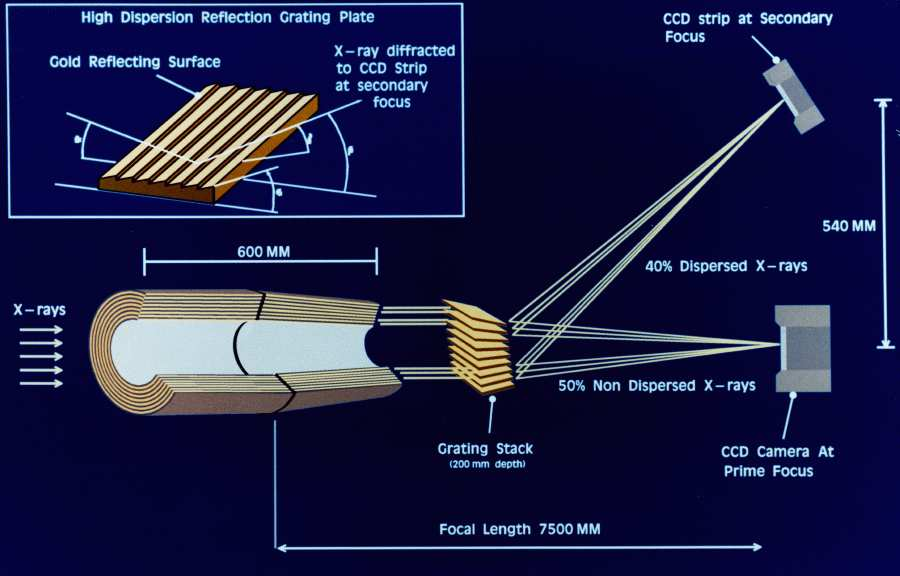
\includegraphics[scale=0.35]{xmm-rgs.png}
		\end{figure}
		
		The XMM-Newton satellite has three telescopes, out of which two are equipped with RGS instruments; these are referred to as RGS1 and RGS2. Each of these RGS instruments comprise of Reflection Grating Assemblies (RGAs) and RGS Focal Cameras (RFCs). These are referred to as \emph{grating stack} and \emph{CCD strip} in figure \ref{xmm-rgs-instrument}.
		
		The light path of the two X-ray telescopes are focussed onto the EPIC MOS cameras at the primary focus. The RGAs intercept $\sim 58\%$ of the light on the light path and diffracts it to the RFCs at the secondary focus. In order to diffract the light, the RGAs have grating plates with groove densities of $\sim 645.6$ lines mm$^{-1}$. This produces the two prominent first and second order spectra with dispersion of 8.3 and 12.7 mm \AA$^{-1}$ at 15 \AA. The performance of various parameters of the RGS instruments, while in orbit, are summarised in the table \ref{xmm-rgs-performance}.
		
		\begin{table}[h!]
			\centering
			\caption{In-orbit performance of RGS instruments}
			\label{xmm-rgs-performance}
			\begin{tabular}{|l|l|c|c|c|c|c|c|}
				\hline
				\multicolumn{2}{|l|}{\multirow{2}{*}{\textbf{Parameter}}} & \multicolumn{3}{c|}{\textbf{RGS1}} & \multicolumn{3}{c|}{\textbf{RGS2}} \\ \cline{3-8}
				\multicolumn{2}{|l|}{} & {10 \AA} & {15 \AA} & {35 \AA} & {10 \AA} & {15 \AA} & {35 \AA} \\ \hline
				\multirow{2}{*}{Effective area (cm$^2$)} & {1$^\text{st}$ order} & {51} & {61} & {21} & {53} & {68} & {25} \\ \cline{2-8}
														 & {2$^\text{nd}$ order} & {29} & {15} & {--} & {31} & {19} & {--} \\ \hline
				\multirow{2}{*}{Resolution (km s$^{-1}$)}& {1$^\text{st}$ order} & {1700} & {1200} & {600} & {1900} & {1400} & {700} \\ \cline{2-8}
														 & {2$^\text{nd}$ order} & {1000} & {700} & {--} & {1200} & {800} & {--} \\ \hline
				\multirow{2}{*}{Wavelength range} & {1$^\text{st}$ order} & \multicolumn{6}{c|}{5 -- 38 \AA (0.35 -- 2.5 keV)} \\ \cline{2-8}
												   & {2$^\text{nd}$ order} & \multicolumn{6}{c|}{5 -- 20 \AA (0.62 -- 2.5 keV)} \\ \hline
				\multirow{2}{*}{Wavelength accuracy} & {1$^\text{st}$ order} & \multicolumn{3}{c|}{$\pm$5 m\AA} & \multicolumn{3}{c|}{$\pm$5 m\AA} \\ \cline{2-8}
                                                  	  & {2$^\text{nd}$ order} & \multicolumn{3}{c|}{$\pm$4 m\AA} & \multicolumn{3}{c|}{$\pm$3 m\AA} \\ \hline
				\multicolumn{2}{|l|}{\multirow{2}{*}{Bin size {[}$3\times 3$ (27 $\mu$)$^2$ pixels{]}}} & \multicolumn{6}{c|}{2.5 arcsec (cross dispersion direction)} \\ \cline{3-8}
				\multicolumn{2}{|l|}{} & \multicolumn{6}{c|}{7 -- 14 m\AA (dispersion direction, first order)} \\ \hline
			\end{tabular}
		\end{table}
		
		The reflection grating used in the RGS instruments diffract into the first and second spectral orders with the highest efficiency -- therefore these two orders produce the most useful data. Even though the third order spectra are present, their count rates are $\sim 8$ times lower than that in the second order. Therefore, the science data provided by the XMM-Newton SOC consists of spectral data from first and second orders only. Table \ref{xmm-rgs-wavelength} summarises the wavelength range covered by the different spectral orders of the RGS instruments.
		\begin{table}[h!]
			\centering
			\caption{Wavelength ranges covered by RGS}
			\label{xmm-rgs-wavelength}
			\begin{tabular}{|c|c|}
				\hline
				{\textbf{Order}} & {\textbf{Wavelength range (\AA)}} \\
				\hline
				{1} & {6 -- 38} \\
				\hline
				{2} & {6 -- 20} \\
				\hline
			\end{tabular}
		\end{table}
	
	\section{Models for Data Fitting} \label{hi-resolution:models}
		Given below in table \ref{xmm-rgs-model-list} is the progression of Xspec models used in the analysis of the RGS spectrum of RX J0925.7-4758. Every model is given a model ID and hereinafter it will be referred to by the same. The progression of the models is evolutionary and follows the same sequence as each was built from the preceding model.
		
		For instance, the first model, i.e. M01 is a simple model which is composed of two model components -- an additive component (\texttt{bbody}) and a multiplicative component (\texttt{tbabs}). This particular model was mainly used to get started with the modelling of the continuum spectrum using a blackbody emission, subjected to absorption. Then, as one progresses downwards along table \ref{xmm-rgs-model-list}, one finds models which are improvements upon the previous model, in terms of the replacement of existing model components or the addition of newer ones.
		\begin{table}[h!]
			\centering
			\caption{List of models used for data fitting}
			\label{xmm-rgs-model-list}
			\begin{tabular}{|l|l|l|}
				\hline
				\textbf{S. No.} & \textbf{Model ID} & \textbf{Xspec model} \\ \hline
				{1} & {M01} & \texttt{tbabs*bbody} \\ \hline
				{2} & {M02} & \texttt{ismabs*bbody} \\ \hline
				{3} & {M03} & \texttt{ismabs*(gauss+bbody)} \\ \hline
				{4} & {M04} & \texttt{ismabs*edge$^3$*(gauss+bbody)} \\ \hline
				{5} & {M05} & \texttt{ismabs*edge$^3$*(mekal+bbody)} \\ \hline
				{6} & {M06} & \texttt{ismabs*(apec+mekal)*swind1} \\ \hline
				{7} & {M07} & \texttt{ismabs*(gauss+mekal+bbody)} \\ \hline
				{8} & {M08} & \texttt{ismabs*(gauss+mekal+bbody)*swind1} \\ \hline
				{9} & {M09} & \texttt{ismabs*(rauch+mekal)*swind1} \\ \hline
				{10} & {M10} & \texttt{ismabs*(rauch+apec)*swind1} \\ \hline
				{11} & {M11} & \texttt{ismabs*(rauch*tbabs+apec+mekal)*swind1} \\ \hline
				{12} & {M12} & \texttt{ismabs*(rauch+apec+mekal)*swind1} \\ \hline
			\end{tabular}
		\end{table}
	
		\subsection{Model Components} \label{hi-resolution:models:components}
		
			\subsubsection{X-ray photoabsorption model: \texttt{ismabs}}
			The \texttt{ismabs} multiplicative model in Xspec provides a way to simulate X-ray photoabsorption \cite{ismabs_gatuzz}. This model incorporates variable columns for both neutral and ionized species from H, He, N, O, Ne, Mg, Si, S, Ar, Ca, Fe, Ni and Zn.
			
			Because of an inherent degeneracy between the relative columns of H, He I, He II, the column density of He I is not included as a free parameter in the model.
			
			In this model, the absorption cross-sections for various species are sourced as follows:
			\begin{itemize}
				\item Neutral states of Si, S, Ar and Ca from Verner et al. \cite{vernerXS}
				\item Singly and doubly ionized states of Si, S, Ar and Ca from Witthoeft et al. \cite{witthoeftXS1,witthoeftXS2}
				\item Neutral, singly and doubly ionized states of N from Garcia et al. \cite{garciaXS1}
				\item Neutral states of O from Gorczyca et al. \cite{gorczycaXS1}
				\item Singly and doubly ionized states of O from Garcia et al. \cite{garciaXS2}, including corrections applied by Gatuzz et al. \cite{gatuzzXS}
				\item Neutral state of Ne from Gorczyca et al. \cite{gorczycaXS2}
				\item Singly and doubly ionized states of Ne from Gorczyca et al. \cite{gorczycaXS3}
				\item For the Fe-L edge region we use the measurement of metallic iron by Kortright \& Kim \cite{kortrightXS}
				\item Neutral, singly and doubly ionized states of Mg from Hasoglu et al. (2014).
			\end{itemize}
			
			The parameters for the \texttt{ismabs} model are given in table \ref{param:ismabs}.
			\begin{table}[h!]
				\centering
				\caption{Model parameters for \texttt{ismabs}}
				\label{param:ismabs}
				\begin{tabular}{|p{3cm}|p{10cm}|}
					\hline
					\textbf{Parameter} & \textbf{Quantity} \\ \hline
					{\texttt{par1}} & {H column (in $10^{22}$ cm$^{-2}$)} \\ \hline
					{\texttt{par2}} & {He II column (in $10^{22}$ cm$^{-2}$)} \\ \hline
					{\texttt{par3}} & {C I column (in $10^{22}$ cm$^{-2}$)} \\ \hline
					{\texttt{par4}} & {C II column (in $10^{22}$ cm$^{-2}$)} \\ \hline
					{\texttt{par5}} & {C III column (in $10^{22}$ cm$^{-2}$)} \\ \hline
					{\texttt{par6}} & {N I column (in $10^{22}$ cm$^{-2}$)} \\ \hline
					{\texttt{par7}} & {N II column (in $10^{22}$ cm$^{-2}$)} \\ \hline
					{\texttt{par8}} & {N III column (in $10^{22}$ cm$^{-2}$)} \\ \hline
					{\texttt{par9}} & {O I column (in $10^{22}$ cm$^{-2}$)} \\ \hline
					{\texttt{par10}} & {O II column (in $10^{22}$ cm$^{-2}$)} \\ \hline
					{\texttt{par11}} & {O III column (in $10^{22}$ cm$^{-2}$)} \\ \hline
					{\texttt{par12}} & {Ne I column (in $10^{22}$ cm$^{-2}$)} \\ \hline
					{\texttt{par13}} & {Ne II column (in $10^{22}$ cm$^{-2}$)} \\ \hline
					{\texttt{par14}} & {Ne III column (in $10^{22}$ cm$^{-2}$)} \\ \hline
					{\texttt{par15}} & {Mg I column (in $10^{22}$ cm$^{-2}$)} \\ \hline
					{\texttt{par16}} & {Mg II column (in $10^{22}$ cm$^{-2}$)} \\ \hline
					{\texttt{par17}} & {Mg III column (in $10^{22}$ cm$^{-2}$)} \\ \hline
					{\texttt{par18}} & {Si I column (in $10^{22}$ cm$^{-2}$)} \\ \hline
					{\texttt{par19}} & {Si II column (in $10^{22}$ cm$^{-2}$)} \\ \hline
					{\texttt{par20}} & {Si III column (in $10^{22}$ cm$^{-2}$)} \\ \hline
					{\texttt{par21}} & {S I column (in $10^{22}$ cm$^{-2}$)} \\ \hline
					{\texttt{par22}} & {S II column (in $10^{22}$ cm$^{-2}$)} \\ \hline
					{\texttt{par23}} & {S III column (in $10^{22}$ cm$^{-2}$)} \\ \hline
					{\texttt{par24}} & {Ar I column (in $10^{22}$ cm$^{-2}$)} \\ \hline
					{\texttt{par25}} & {Ar II column (in $10^{22}$ cm$^{-2}$)} \\ \hline
					{\texttt{par26}} & {Ar III column (in $10^{22}$ cm$^{-2}$)} \\ \hline
					{\texttt{par27}} & {Ca I column (in $10^{22}$ cm$^{-2}$)} \\ \hline
					{\texttt{par28}} & {Ca II column (in $10^{22}$ cm$^{-2}$)} \\ \hline
					{\texttt{par29}} & {Ca III column (in $10^{22}$ cm$^{-2}$)} \\ \hline
					{\texttt{par30}} & {Fe column (in $10^{22}$ cm$^{-2}$)} \\ \hline
					{\texttt{par31}} & {Redshift $z$} \\ \hline
				\end{tabular}
			\end{table}
			
			\subsubsection{Astrophysical plasma emission code: \texttt{apec}}
				The \texttt{apec} additive model in Xspec simulates an emission spectrum that is obtained from a collisionally-ionized diffuse gas \cite{smithAPEC}. The atomic data for collisional and radiative rates, recombination cross sections, dielectronic recombination rates, and satellite line wavelengths are taken from the Astrophysical Plasma Emission Database (APED).
			
				The \texttt{apec} model provides a way to create emission models for plasma, which can be used to analyse spectral data from high-resolution X-ray spectrometers, as in the case of XMM-Newton or Chandra. The current version of the code stores the atomic data in FITS files, thereby separating it from the code. This optimizes limitations on the speed and memory across different computers.
			
				The \texttt{apec} model simulates a hot, optically thin plasma which is in a collisional ionization equilibrium, and computes both resulting continuum and line emissivities. Here, the \textit{emissivity} of a spectral line is defined as the  total number of radiative transitions per unit volume divided by the product of the electron density $n_e$ and the hydrogen (neutrals and protons) density $n_H$ in the astrophysical plasma, resulting in line emissivities having units of cm$^3$ s$^{-1}$.
			
				The parameters for the \texttt{apec} model are given in table \ref{param:apec}.
				\begin{table}[h!]
					\centering
					\caption{Model parameters for \texttt{apec}}
					\label{param:apec}
					\begin{tabular}{|p{3cm}|p{10cm}|}
						\hline
						\textbf{Parameter} & \textbf{Quantity} \\ \hline
						{\texttt{par1}} & {Plasma temperature (in keV)} \\ \hline
						{\texttt{par2}} & {Abundances of the metals C, N, O, Ne, Mg, Al, Si, S, Ar, Ca, Fe, Ni} \\ \hline
						{\texttt{par3}} & {Redshift $z$} \\ \hline
						{\texttt{norm}} & {Normalization of the component computed as $\displaystyle\dfrac{10^{-14}}{4\pi[D_A(1+z)]^2}\int{n_en_H\diff{V}}$, where $D_A$ is the angular diameter distance to the source (in cm), $n_e$ and $n_H$ are the electron densities (in cm$^{-3}$) respectively} \\ \hline
					\end{tabular}
				\end{table}

			\subsubsection{Model for emission due to optically-thin plasma: \texttt{mekal}}
				The additive model \texttt{mekal} in Xspec allows the simulation of an emission spectrum due to a diffuse plasma, whose electrons have a Maxwellian energy distribution. This model uses the spectral line list as calculated by Mewe and Kaastra \cite{meka}, additional calculations for L-shell of Fe ions by Liedahl et al. \cite{liedahl}. The model provides the option to either calculate the spectrum by running the \texttt{mekal} code, or by interpolation on a pre-calculated \texttt{mekal} table, or simply by using the AtomDB data.
				
				The models \texttt{mekal} and \texttt{apec} both simulate emission due to optically-thin plasma, the difference being in the methodology of calculation of the line lists.
				
				The parameters for the \texttt{mekal} model are given in table \ref{param:mekal}.
				\begin{table}[h!]
					\centering
					\caption{Model parameters for \texttt{mekal}}
					\label{param:mekal}
					\begin{tabular}{|p{3cm}|p{10cm}|}
						\hline
						\textbf{Parameter} & \textbf{Quantity} \\ \hline
						{\texttt{par1}} & {Plasma temperature (in keV)} \\ \hline
						{\texttt{par2}} & {H density (in cm$^{-3}$)} \\ \hline
						{\texttt{par3}} & {Metal abundances for the elements C, N, O, Ne, Na, Mg, Al, Si, S, Ar, Ca, Fe, Ni} \\ \hline
						{\texttt{par4}} & {Redshift $z$} \\ \hline
						{\texttt{par5}} & {Switch between \texttt{mekal} calculation (0), interpolation (1) and interpolation using AtomDB data (2)} \\ \hline
						{\texttt{norm}} & {Normalization of the component computed as $\displaystyle\dfrac{10^{-14}}{4\pi[D_A(1+z)]^2}\int{n_en_H\diff{V}}$, where $D_A$ is the angular diameter distance to the source (in cm), $n_e$ and $n_H$ are the electron densities (in cm$^{-3}$) respectively} \\ \hline
					\end{tabular}
				\end{table}
			
			\subsubsection{Velocity shear absorption: \texttt{swind1}}
				Originally meant for AGN spectra, the \texttt{swind1} multiplicative model fits the soft excess in partially ionized absorbing material with a large velocity shear. This is approximated by the model component by using XSTAR kn5 photoionization absorption model grids, which were calculated assuming a micro-turbulence of 100 km/s, and subsequently convolving with Gaussian smearing \cite{swind1}.
				
				In this work, the \texttt{swind1} component is used as a proxy model for possible stellar wind from the source RX J0925.7-4758, which may be indicated by the presence of P Cygni profiles in its spectrum.
				
				The parameters for the \texttt{swind1} model are given in table \ref{param:swind1}.
				\begin{table}[h!]
					\centering
					\caption{Model parameters for \texttt{swind1}}
					\label{param:swind1}
					\begin{tabular}{|p{3cm}|p{10cm}|}
						\hline
						\textbf{Parameter} & \textbf{Quantity} \\ \hline
						{\texttt{par1}} & {Column density (in $10^{22}$ cm$^{-2}$)} \\ \hline
						{\texttt{par2}} & {$\log{\xi}$ where $\xi=L/nr^2$} \\ \hline
						{\texttt{par3}} & {$\sigma$: Gaussian $\sigma$ for velocity smearing ($v/c$)} \\ \hline
						{\texttt{par4}} & {Redshift $z$} \\ \hline
					\end{tabular}
				\end{table}
			
			\subsubsection{T\"{u}bingen NLTE Model-Atmosphere Package: \texttt{rauch}}
				The T\"{u}bingen NLTE Model-Atmosphere Package (TMAP) is a tool to calculate stellar atmospheres in spherical or plane-parallel geometry in hydrostatic and radiative equilibrium allowing departures from local thermodynamic equilibrium (LTE) for the population of atomic levels \cite{wernerDreizler}. TMAP is based on the so-called Accelerated Lambda Iteration (ALI) method and is able to account for line blanketing by metals \cite{rauchALI}. All elements from hydrogen to nickel may be included in the calculation with model atoms which are tailored for the aims of the user \cite{wernerTMAP}.
				
				The web-link to a set of theoretical spectral energy distributions (SEDs) of TMAP NLTE model atmospheres were provided by Rauch \cite{rauchFITS}, which contained a grid of 10 FITS files for varying temperatures. The abundances of various elements for this grid are given in table \ref{rauch:abundances}. The TMAP model series refer to the files corresponding to the model atmosphere grid, with each column named after the last three characters of the FITS filename. The grid is calculated for effective temperatures in the range $4.50\times 10^5\,\text{K}\leqslant T_\text{eff}\leqslant 1.05\times 10^6\,\text{K}$ in steps $\Delta T=10^4\,\text{K}$. The effective surface gravity is $\log_{10}{g}=9$. The fluxes in the SEDs are calculated using the TMAP code from models with different elemental abundance ratios $[X]$.
				
				\begin{table}[h!]
					\centering
					\caption{Elemental abundances for TMAP grid}
					\label{rauch:abundances}
					\begin{tabular}{|c|cccccccccc|}
						\hline
						\multirow{2}{*}{\textbf{{[}X{]}}} & \multicolumn{10}{c|}{\textbf{TMAP model series}} \\ \cline{2-11} & \multicolumn{1}{c|}{\textbf{003}} & \multicolumn{1}{c|}{\textbf{004}} & \multicolumn{1}{c|}{\textbf{005}} & \multicolumn{1}{c|}{\textbf{006}} & \multicolumn{1}{c|}{\textbf{007}} & \multicolumn{1}{c|}{\textbf{008}} & \multicolumn{1}{c|}{\textbf{009}} & \multicolumn{1}{c|}{\textbf{010}} & \multicolumn{1}{c|}{\textbf{011}} & \textbf{201} \\ \hline
						{[}H{]} & \multicolumn{1}{c|}{-0.688} & \multicolumn{1}{c|}{-0.683} & \multicolumn{1}{c|}{-0.677} & \multicolumn{1}{c|}{-0.673} & \multicolumn{1}{c|}{-0.672} & \multicolumn{1}{c|}{-0.671} & \multicolumn{1}{c|}{-0.670} & \multicolumn{1}{c|}{-0.670} & \multicolumn{1}{c|}{-0.669} & -0.885 \\ \hline
						{[}He{]} & \multicolumn{1}{c|}{0.382} & \multicolumn{1}{c|}{0.387} & \multicolumn{1}{c|}{0.393} & \multicolumn{1}{c|}{0.397} & \multicolumn{1}{c|}{0.398} & \multicolumn{1}{c|}{0.399} & \multicolumn{1}{c|}{0.400} & \multicolumn{1}{c|}{0.401} & \multicolumn{1}{c|}{0.401} & 0.489 \\ \hline
						{[}C{]} & \multicolumn{1}{c|}{-1.513} & \multicolumn{1}{c|}{-1.073} & \multicolumn{1}{c|}{-0.772} & \multicolumn{1}{c|}{-0.675} & \multicolumn{1}{c|}{-0.596} & \multicolumn{1}{c|}{-0.529} & \multicolumn{1}{c|}{-0.471} & \multicolumn{1}{c|}{-0.420} & \multicolumn{1}{c|}{-0.374} & -0.057 \\ \hline
						{[}N{]} & \multicolumn{1}{c|}{1.803} & \multicolumn{1}{c|}{1.678} & \multicolumn{1}{c|}{1.460} & \multicolumn{1}{c|}{1.159} & \multicolumn{1}{c|}{1.062} & \multicolumn{1}{c|}{0.937} & \multicolumn{1}{c|}{0.761} & \multicolumn{1}{c|}{0.460} & \multicolumn{1}{c|}{0.159} & 1.668 \\ \hline
						{[}O{]} & \multicolumn{1}{c|}{1.528} & \multicolumn{1}{c|}{1.533} & \multicolumn{1}{c|}{1.538} & \multicolumn{1}{c|}{1.543} & \multicolumn{1}{c|}{1.544} & \multicolumn{1}{c|}{1.544} & \multicolumn{1}{c|}{1.545} & \multicolumn{1}{c|}{1.546} & \multicolumn{1}{c|}{1.547} & 1.206 \\ \hline
						{[}Ne{]} & \multicolumn{1}{c|}{-0.474} & \multicolumn{1}{c|}{-0.469} & \multicolumn{1}{c|}{-0.464} & \multicolumn{1}{c|}{-0.459} & \multicolumn{1}{c|}{-0.459} & \multicolumn{1}{c|}{-0.458} & \multicolumn{1}{c|}{-0.457} & \multicolumn{1}{c|}{-0.456} & \multicolumn{1}{c|}{-0.456} & -0.517 \\ \hline
						{[}Mg{]} & \multicolumn{1}{c|}{-0.454} & \multicolumn{1}{c|}{-0.450} & \multicolumn{1}{c|}{-0.444} & \multicolumn{1}{c|}{-0.439} & \multicolumn{1}{c|}{-0.439} & \multicolumn{1}{c|}{-0.438} & \multicolumn{1}{c|}{-0.437} & \multicolumn{1}{c|}{-0.436} & \multicolumn{1}{c|}{-0.436} & -0.497 \\ \hline
						{[}Si{]} & \multicolumn{1}{c|}{0.167} & \multicolumn{1}{c|}{0.172} & \multicolumn{1}{c|}{0.178} & \multicolumn{1}{c|}{0.182} & \multicolumn{1}{c|}{0.183} & \multicolumn{1}{c|}{0.184} & \multicolumn{1}{c|}{0.185} & \multicolumn{1}{c|}{0.186} & \multicolumn{1}{c|}{0.186} & 0.125 \\ \hline
						{[}S{]} & \multicolumn{1}{c|}{-1.583} & \multicolumn{1}{c|}{-1.578} & \multicolumn{1}{c|}{-1.573} & \multicolumn{1}{c|}{-1.568} & \multicolumn{1}{c|}{-1.567} & \multicolumn{1}{c|}{-1.567} & \multicolumn{1}{c|}{-1.566} & \multicolumn{1}{c|}{-1.565} & \multicolumn{1}{c|}{-1.565} & -1.625 \\ \hline
						{[}IG{]} & \multicolumn{1}{c|}{0.828} & \multicolumn{1}{c|}{0.833} & \multicolumn{1}{c|}{0.838} & \multicolumn{1}{c|}{0.843} & \multicolumn{1}{c|}{0.843} & \multicolumn{1}{c|}{0.844} & \multicolumn{1}{c|}{0.845} & \multicolumn{1}{c|}{0.846} & \multicolumn{1}{c|}{0.846} & 0.786 \\ \hline
					\end{tabular}
				\end{table}
				
				The quantity $[X]$ is logarithmic and is calculated as
				\begin{align}
					\label{rauch:[X]}
					[X]=\log{\left(\dfrac{\text{stellar mass fraction}}{\text{solar mass fraction}}\right)}=\log{\left(\dfrac{X_*}{X_\odot}\right)}
				\end{align}
				
				For any element $X$ denotes its mass fraction which is defined as $X\equiv\dfrac{m_X}{M}$, where $m_X$ is the mass of the element and $M$ is the total mass of the system. For example in table \ref{rauch:abundances},
				\begin{align*}
					[X]&=-0.675 \\
					\implies \log_{10}\left(\dfrac{X_*}{X_\odot}\right)&=-0.675 \\
					\implies \dfrac{X_*}{X_\odot}&=10^{-0.675} \\
					\implies X_*&=0.211X_\odot
				\end{align*}
				That is, $[X]$ indicates that the stellar mass fraction $X_*$ for that element is about 21\% that of solar mass fraction $X_\odot$.
				
				The parameters for the \texttt{rauch} model are given in table \ref{param:rauch}.
				\begin{table}[h!]
					\centering
					\caption{Model parameters for \texttt{rauch}}
					\label{param:rauch}
					\begin{tabular}{|p{3cm}|p{10cm}|}
						\hline
						\textbf{Parameter} & \textbf{Quantity} \\ \hline
						{\texttt{par1}} & {Effective temperature $T$ (in K)} \\ \hline
						{\texttt{par2}} & {Redshift $z$} \\ \hline
						{\texttt{norm}} & {Normalization of the component computed as $\displaystyle\dfrac{10^{-14}}{4\pi[D_A(1+z)]^2}\int{n_en_H\diff{V}}$, where $D_A$ is the angular diameter distance to the source (in cm), $n_e$ and $n_H$ are the electron densities (in cm$^{-3}$) respectively} \\ \hline
					\end{tabular}
				\end{table}
	
	\section{Analysis of RGS Spectra} \label{hi-resolution:analysis}
		Both the spectra of RX J0925.7-4758 obtained by the RGS instrument of XMM-Newton were analyzed using a subset of models from the list given in table \ref{xmm-rgs-model-list}. Models with IDs M07, M08, M09, M10, M11 and M12 were applied on the RGS data for both spectral orders.
		
		\subsection{Fitting of RGS1 Spectra} \label{hi-resolution:analysis:rgs1}
			The best fits for both diffraction orders were obtained using the model M11, i.e.
			\begin{center}
				\texttt{ismabs*(rauch*tbabs+apec+mekal)*swind1}
			\end{center}
			All the other models, though with $\chi^2_\text{red}$ outside the acceptable range, seemingly yield fits which are better than those in current literature. The trend shown by the $\chi^2_\text{red}$ across all the models considered here are shown in figure \ref{fig:mrvel-rgs1-chisq}.
			
			\begin{figure}[h!]
				\centering
				\caption{$\chi^2_\text{red}$ trend for RX J0925.7-4758 spectra from RGS1 instrument}
				\label{fig:mrvel-rgs1-chisq}
				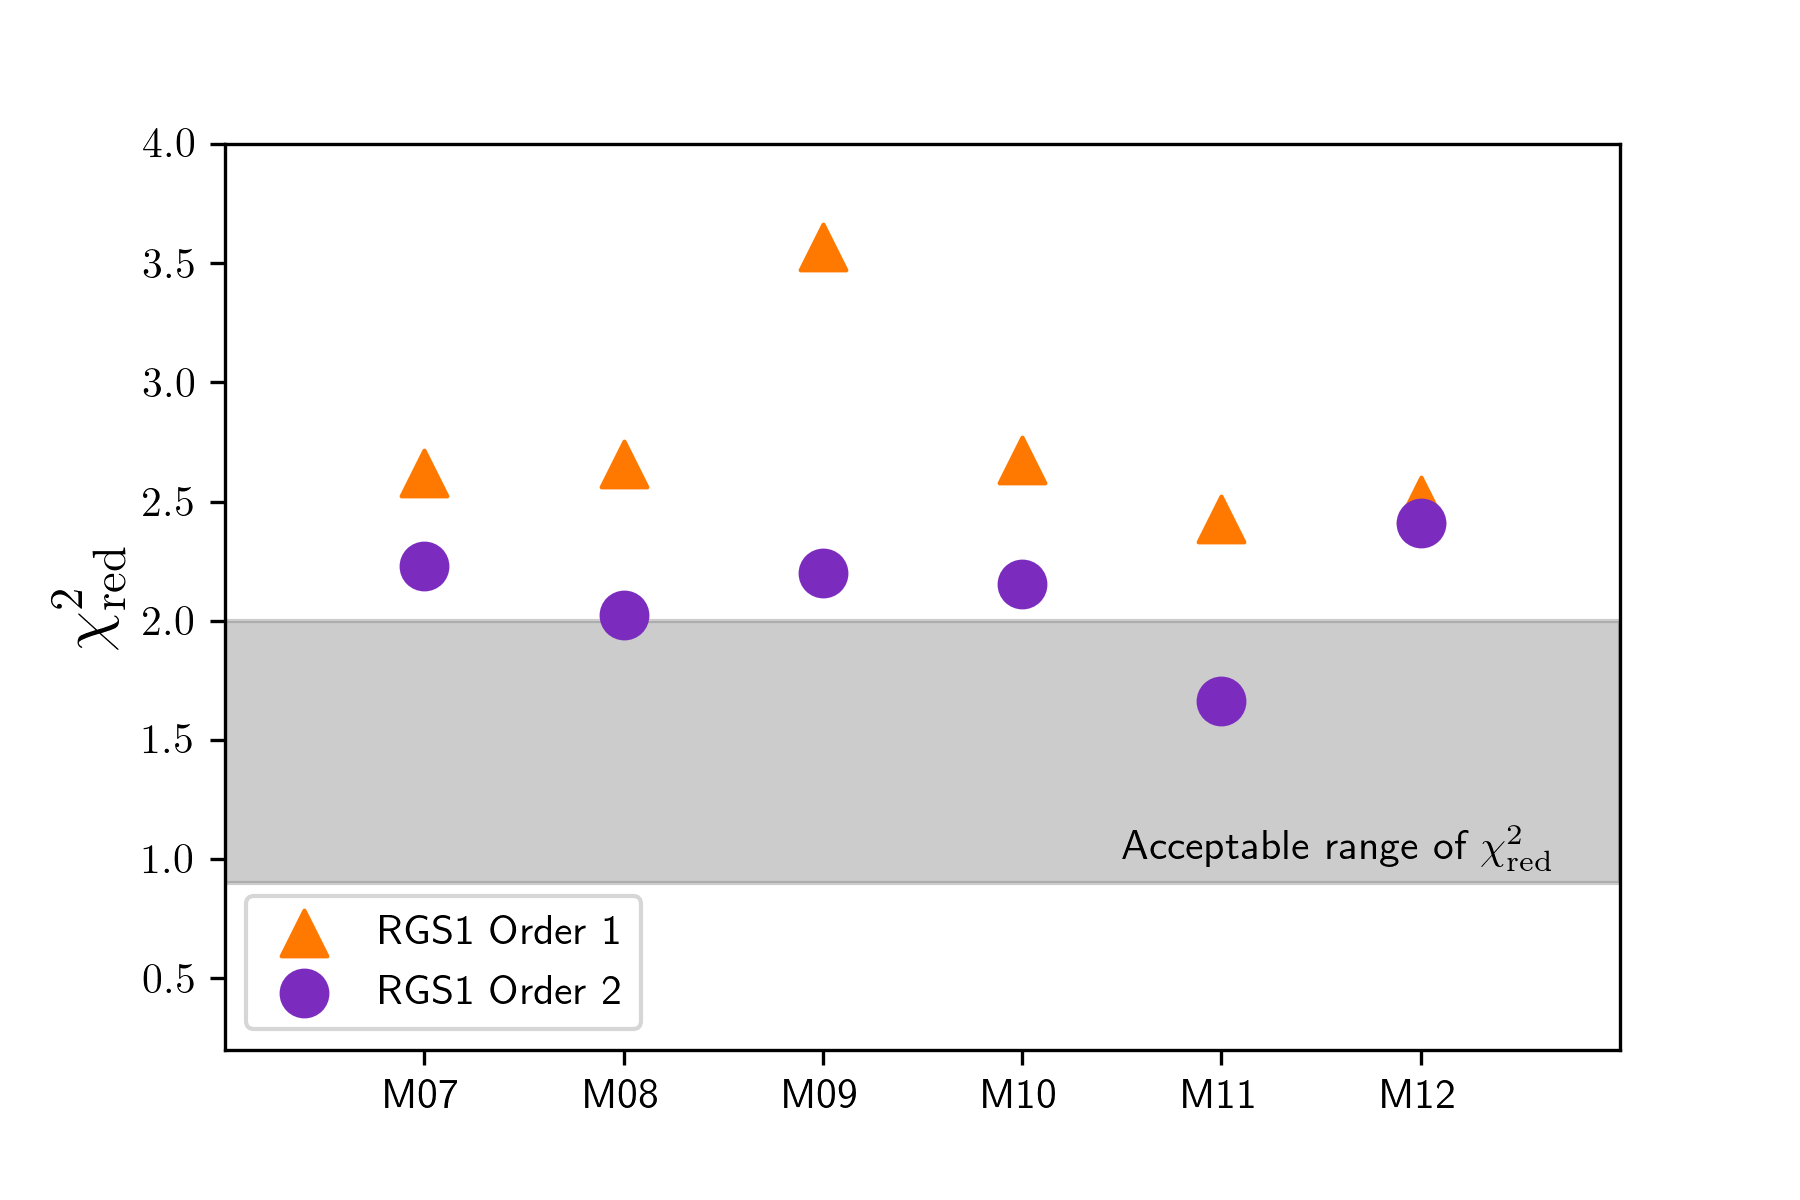
\includegraphics[width=0.85\textwidth]{mrvel-rgs1-chisq}
			\end{figure}
		
			The fitted spectra, along with the residuals are displayed as follows:
			\begin{figure}[h!]
				\centering
				\caption{Spectral fits for RGS1 spectra using model M07}
				\label{xmm:rgs1-m07}
				\subfloat[Order 1 \label{xmm:rgs1-m07:o1}]{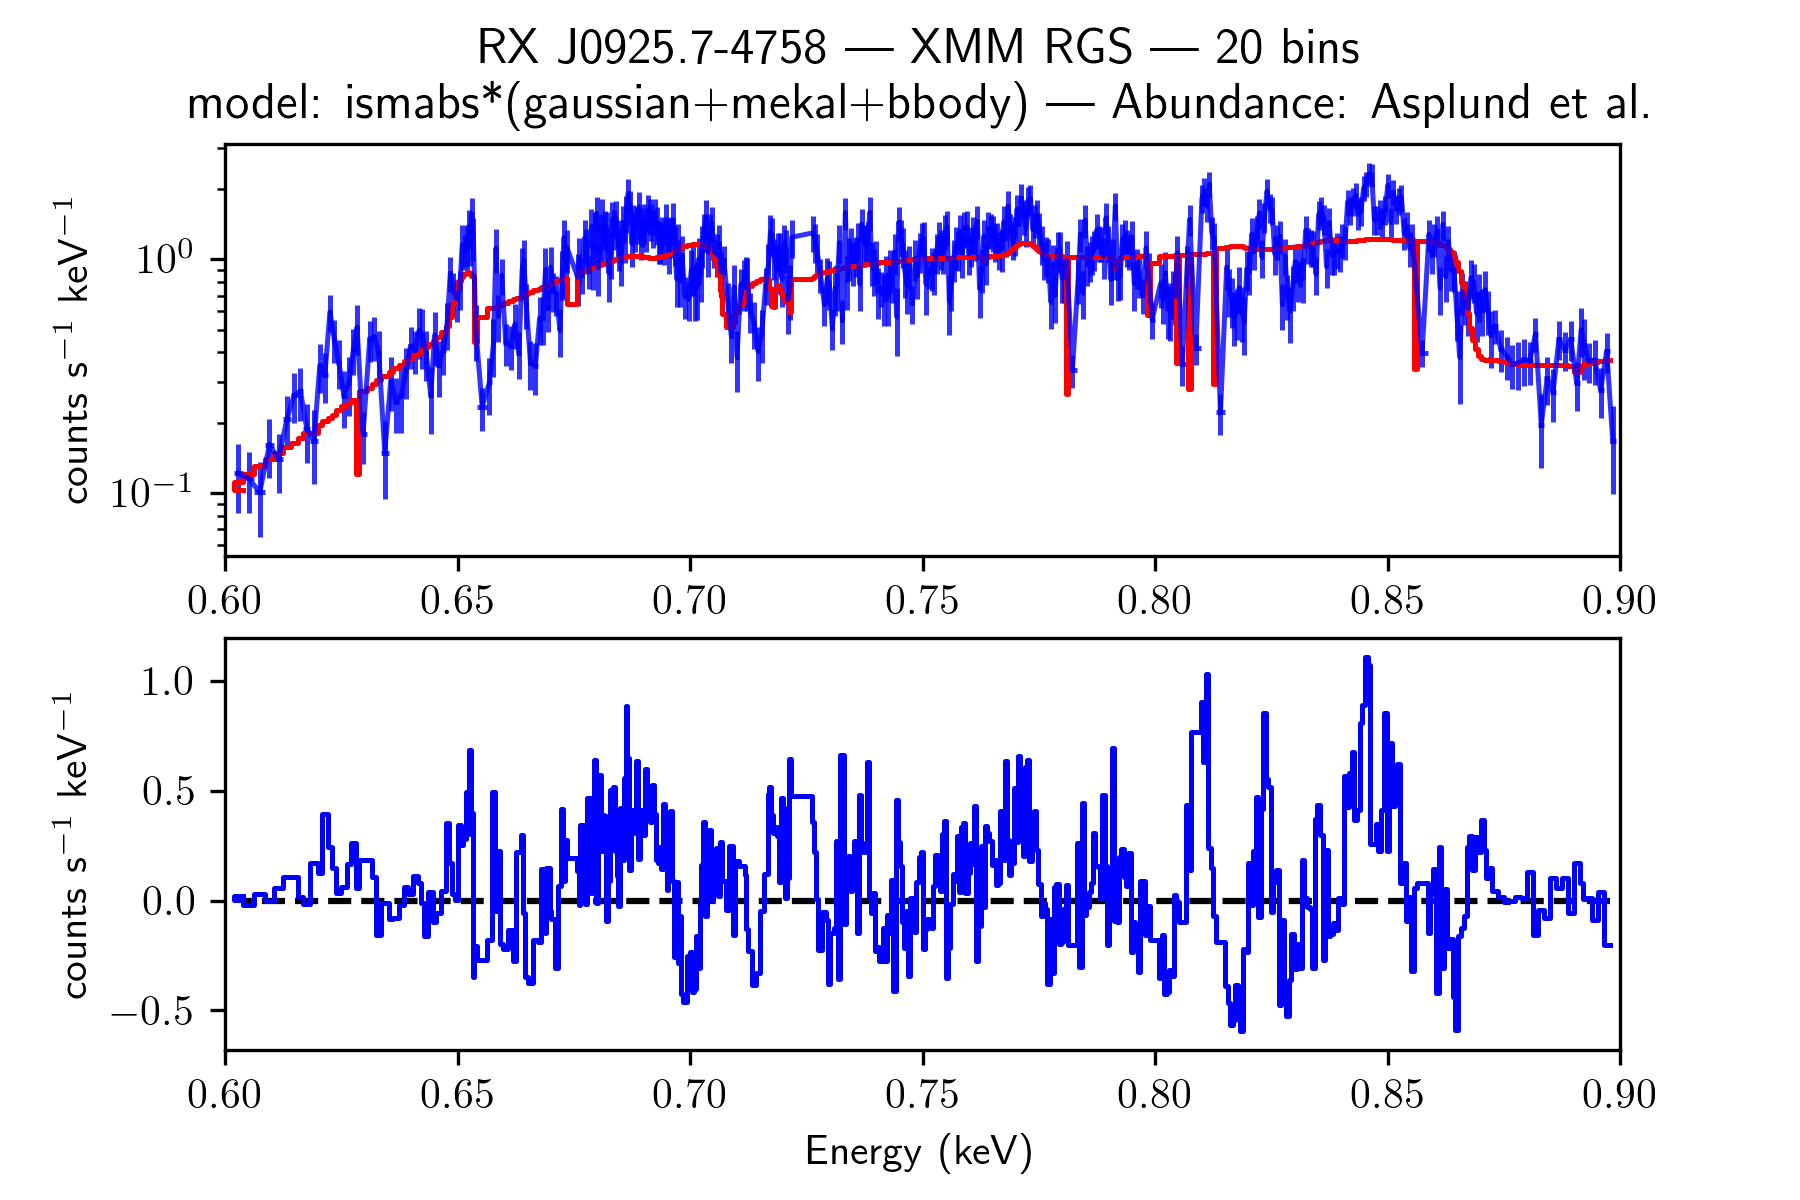
\includegraphics[width=0.45\textwidth]{mrvel-rgs1-o1-m07}} %\hfill
				\subfloat[Order 2 \label{xmm:rgs1-m07:o2}]{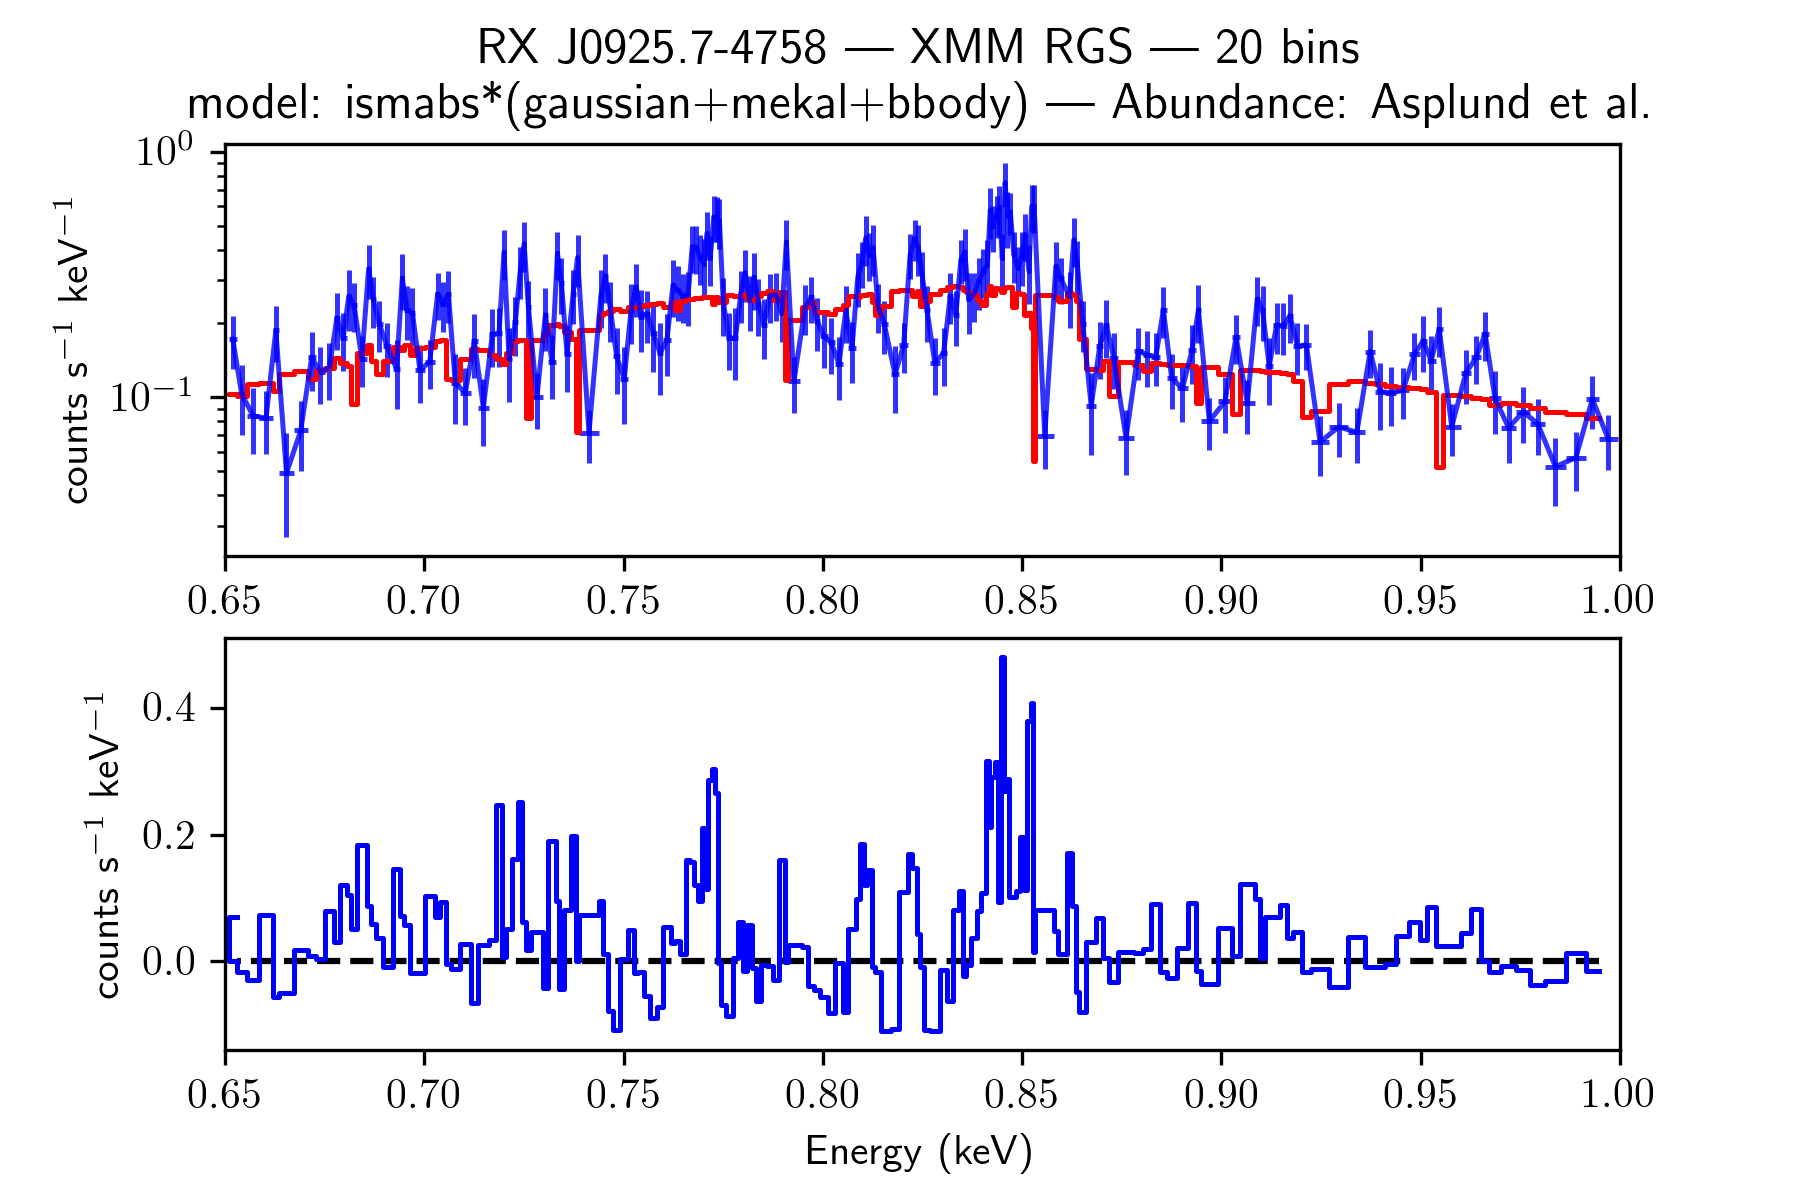
\includegraphics[width=0.45\textwidth]{mrvel-rgs1-o2-m07}} %\hfill
			\end{figure}
			\begin{figure}[h!]
				\centering
				\caption{Spectral fits for RGS1 spectra using model M08}
				\label{xmm:rgs1-m08}
				\subfloat[Order 1 \label{xmm:rgs1-m08:o1}]{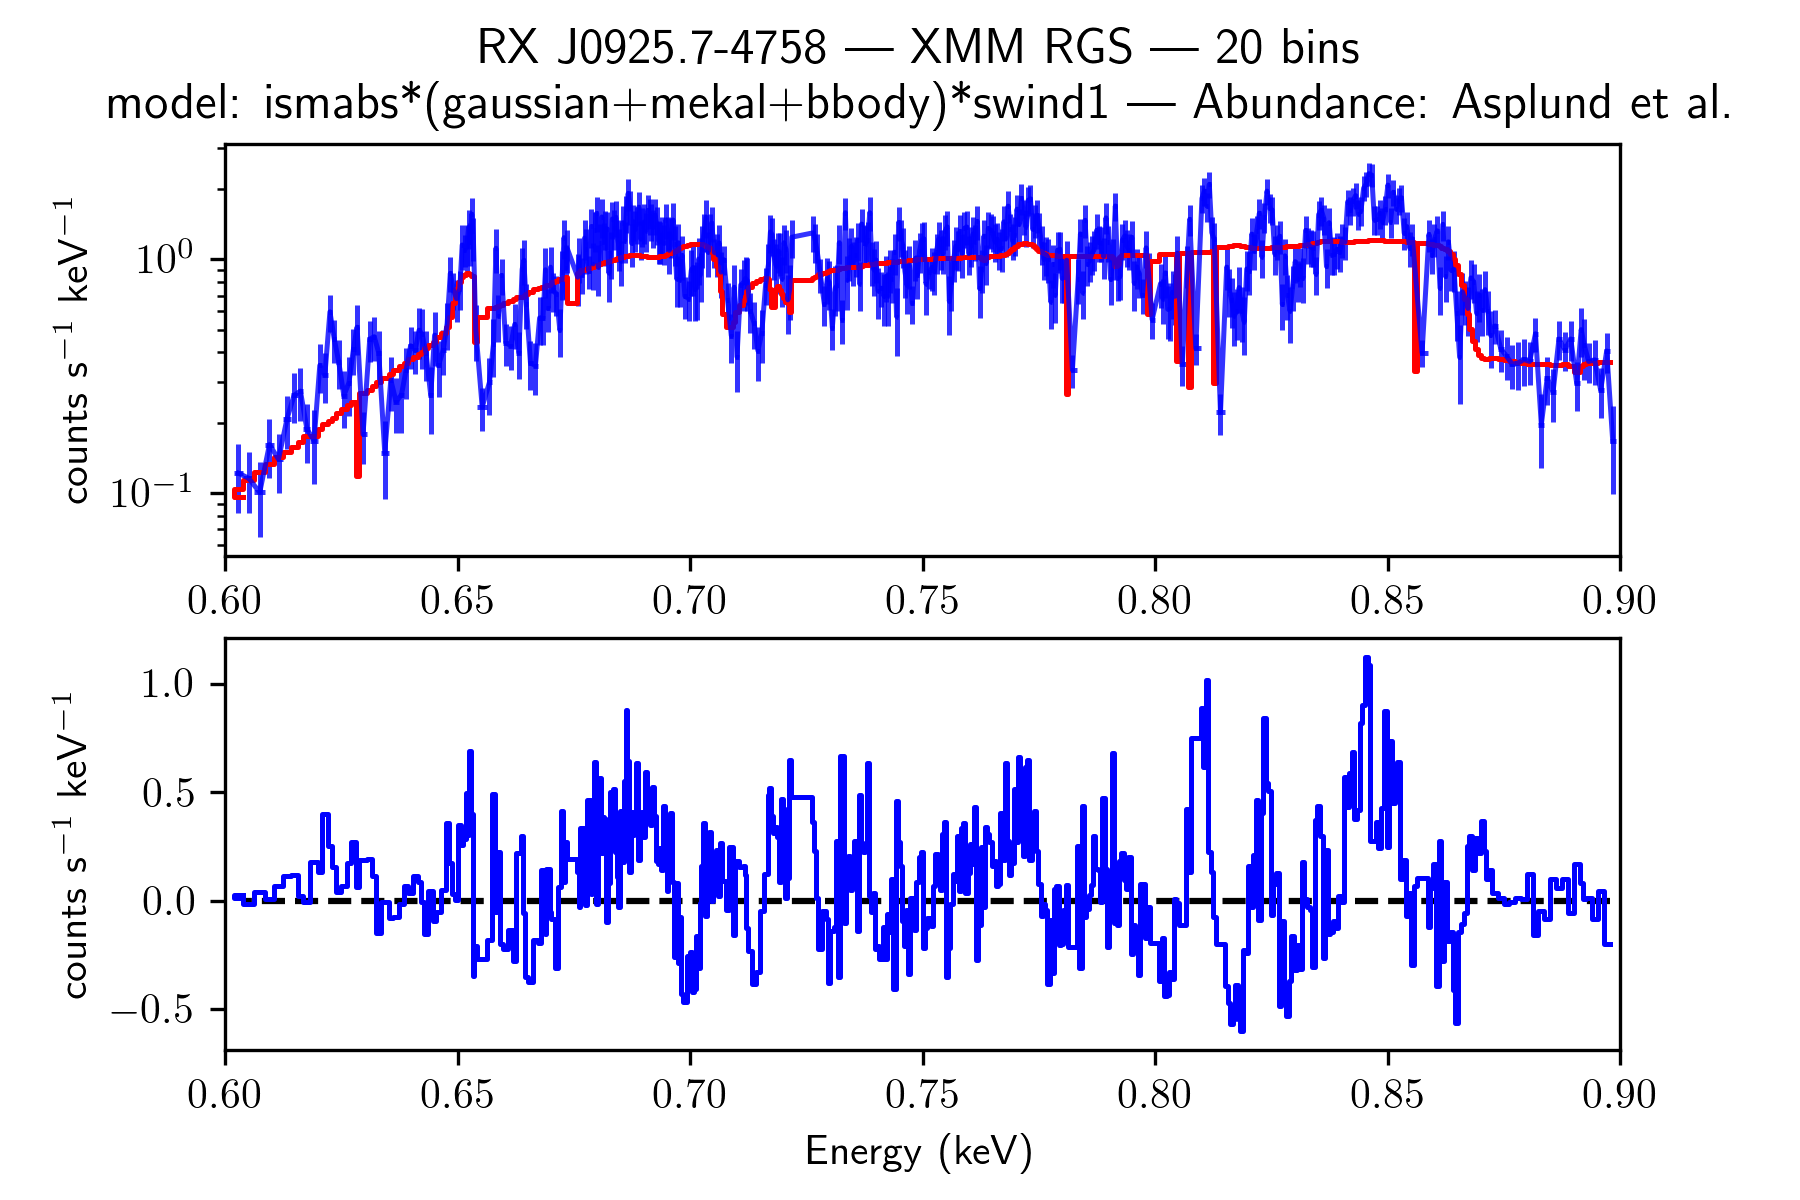
\includegraphics[width=0.45\textwidth]{mrvel-rgs1-o1-m08}} %\hfill
				\subfloat[Order 2 \label{xmm:rgs1-m08:o2}]{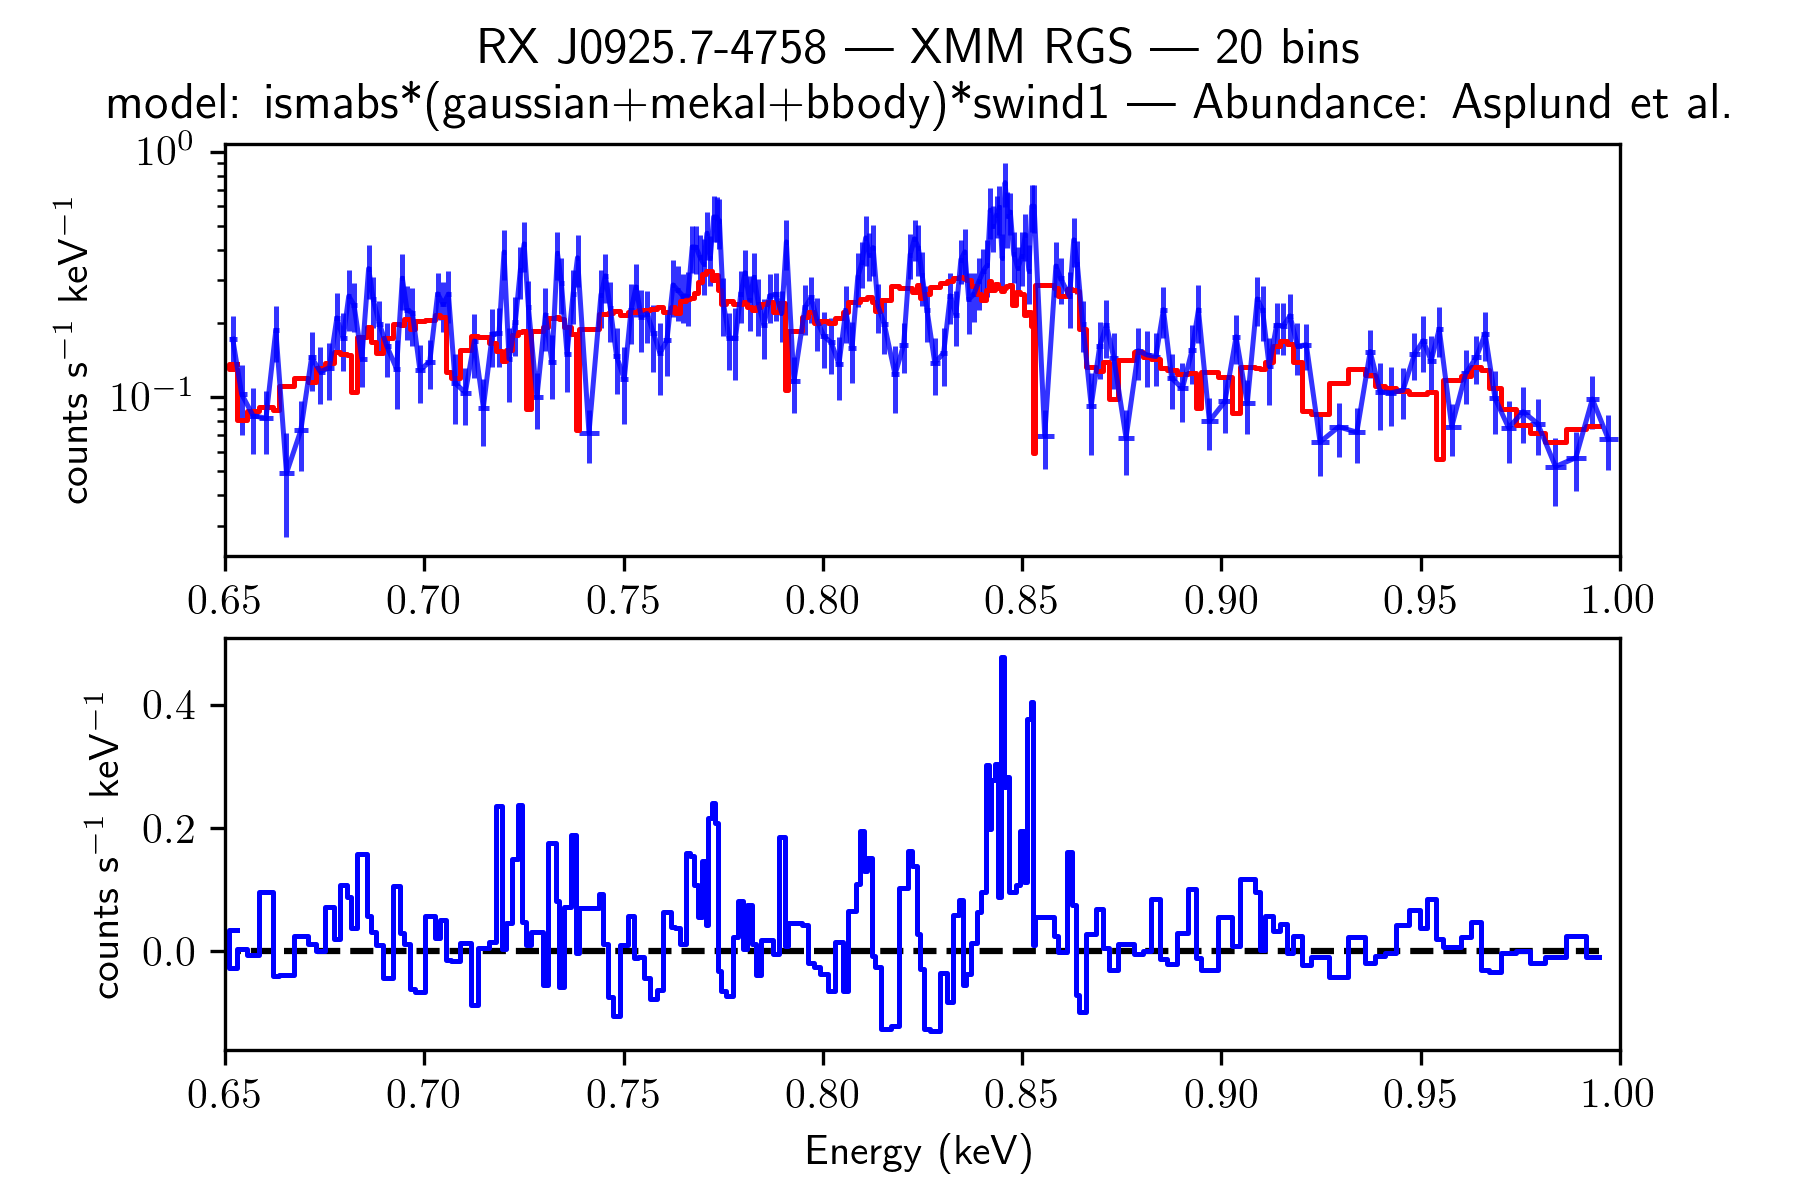
\includegraphics[width=0.45\textwidth]{mrvel-rgs1-o2-m08}} %\hfill
			\end{figure}
			\begin{figure}[h!]
				\centering
				\caption{Spectral fits for RGS1 spectra using model M09}
				\label{xmm:rgs1-m09}
				\subfloat[Order 1 \label{xmm:rgs1-m09:o1}]{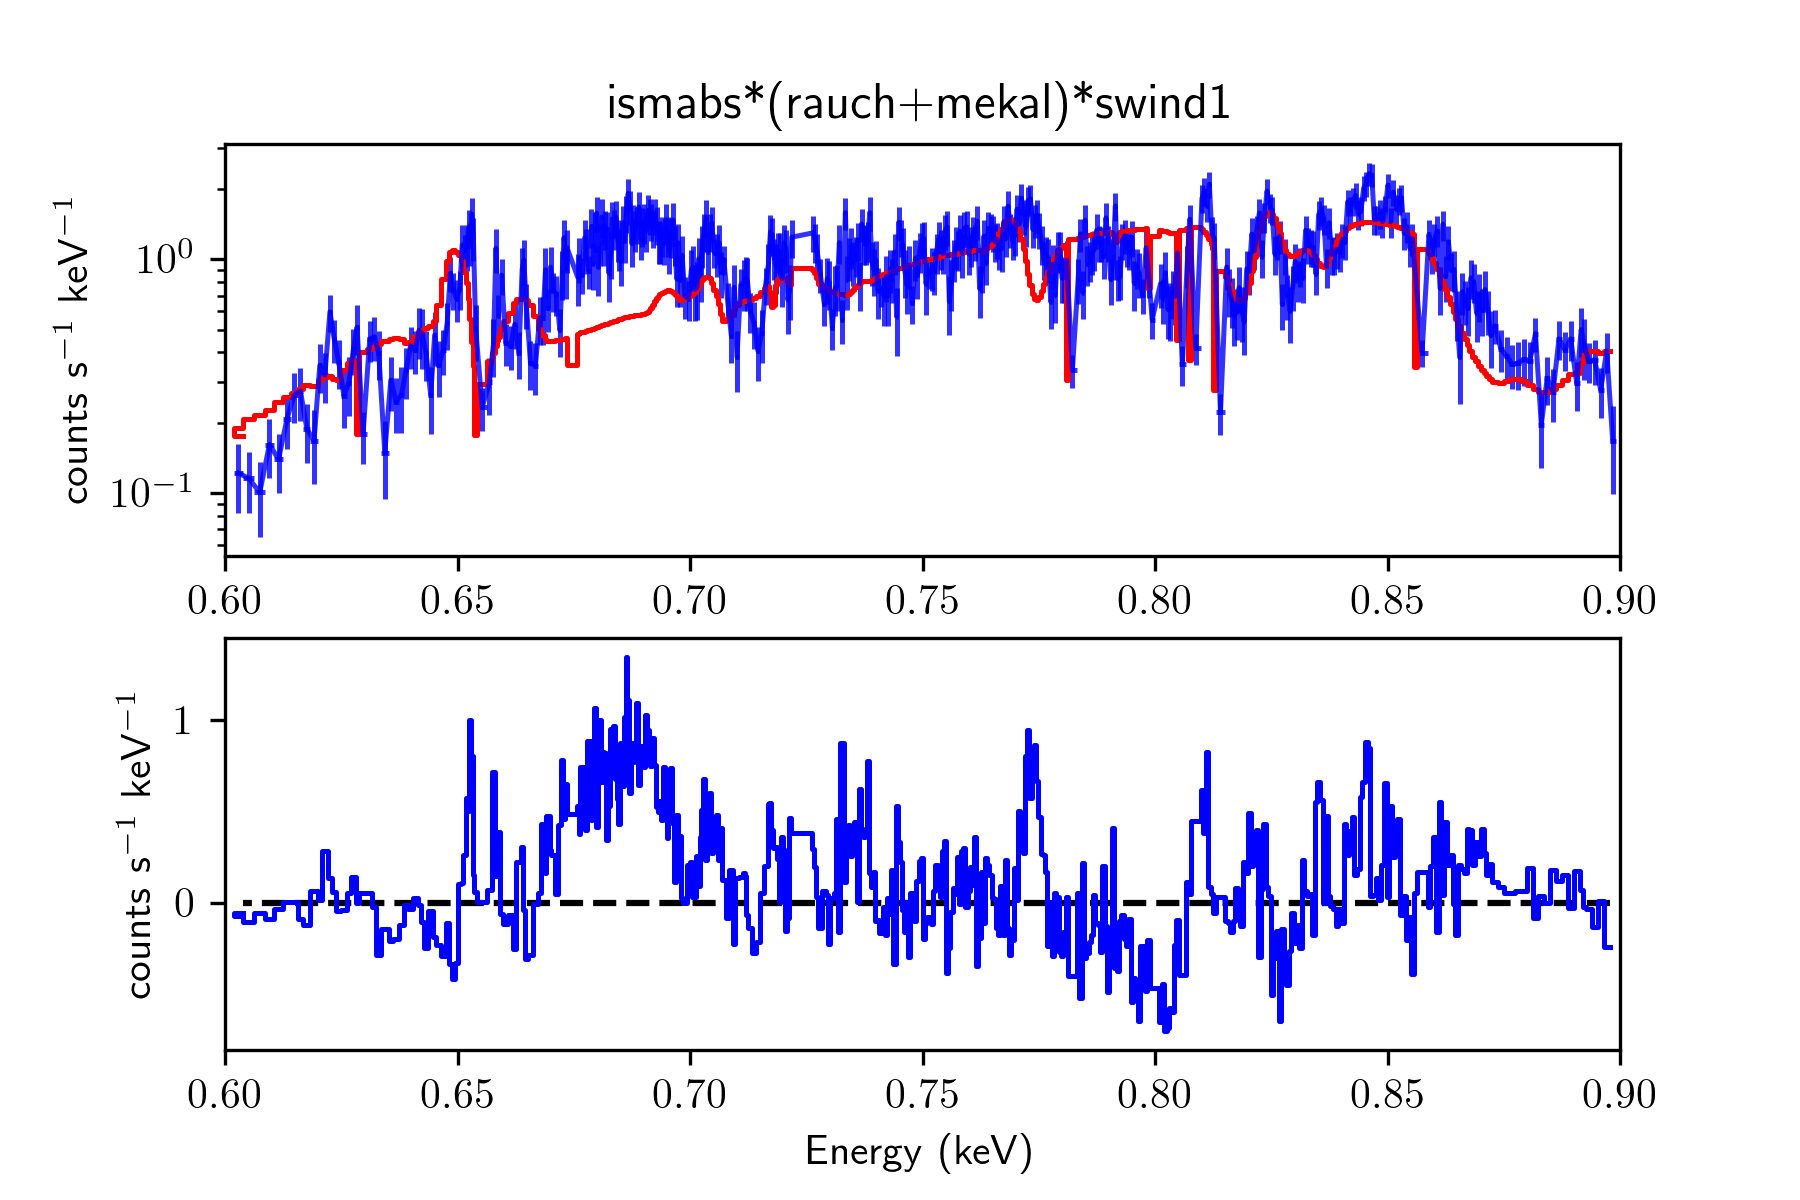
\includegraphics[width=0.45\textwidth]{mrvel-rgs1-o1-m09}} %\hfill
				\subfloat[Order 2 \label{xmm:rgs1-m09:o2}]{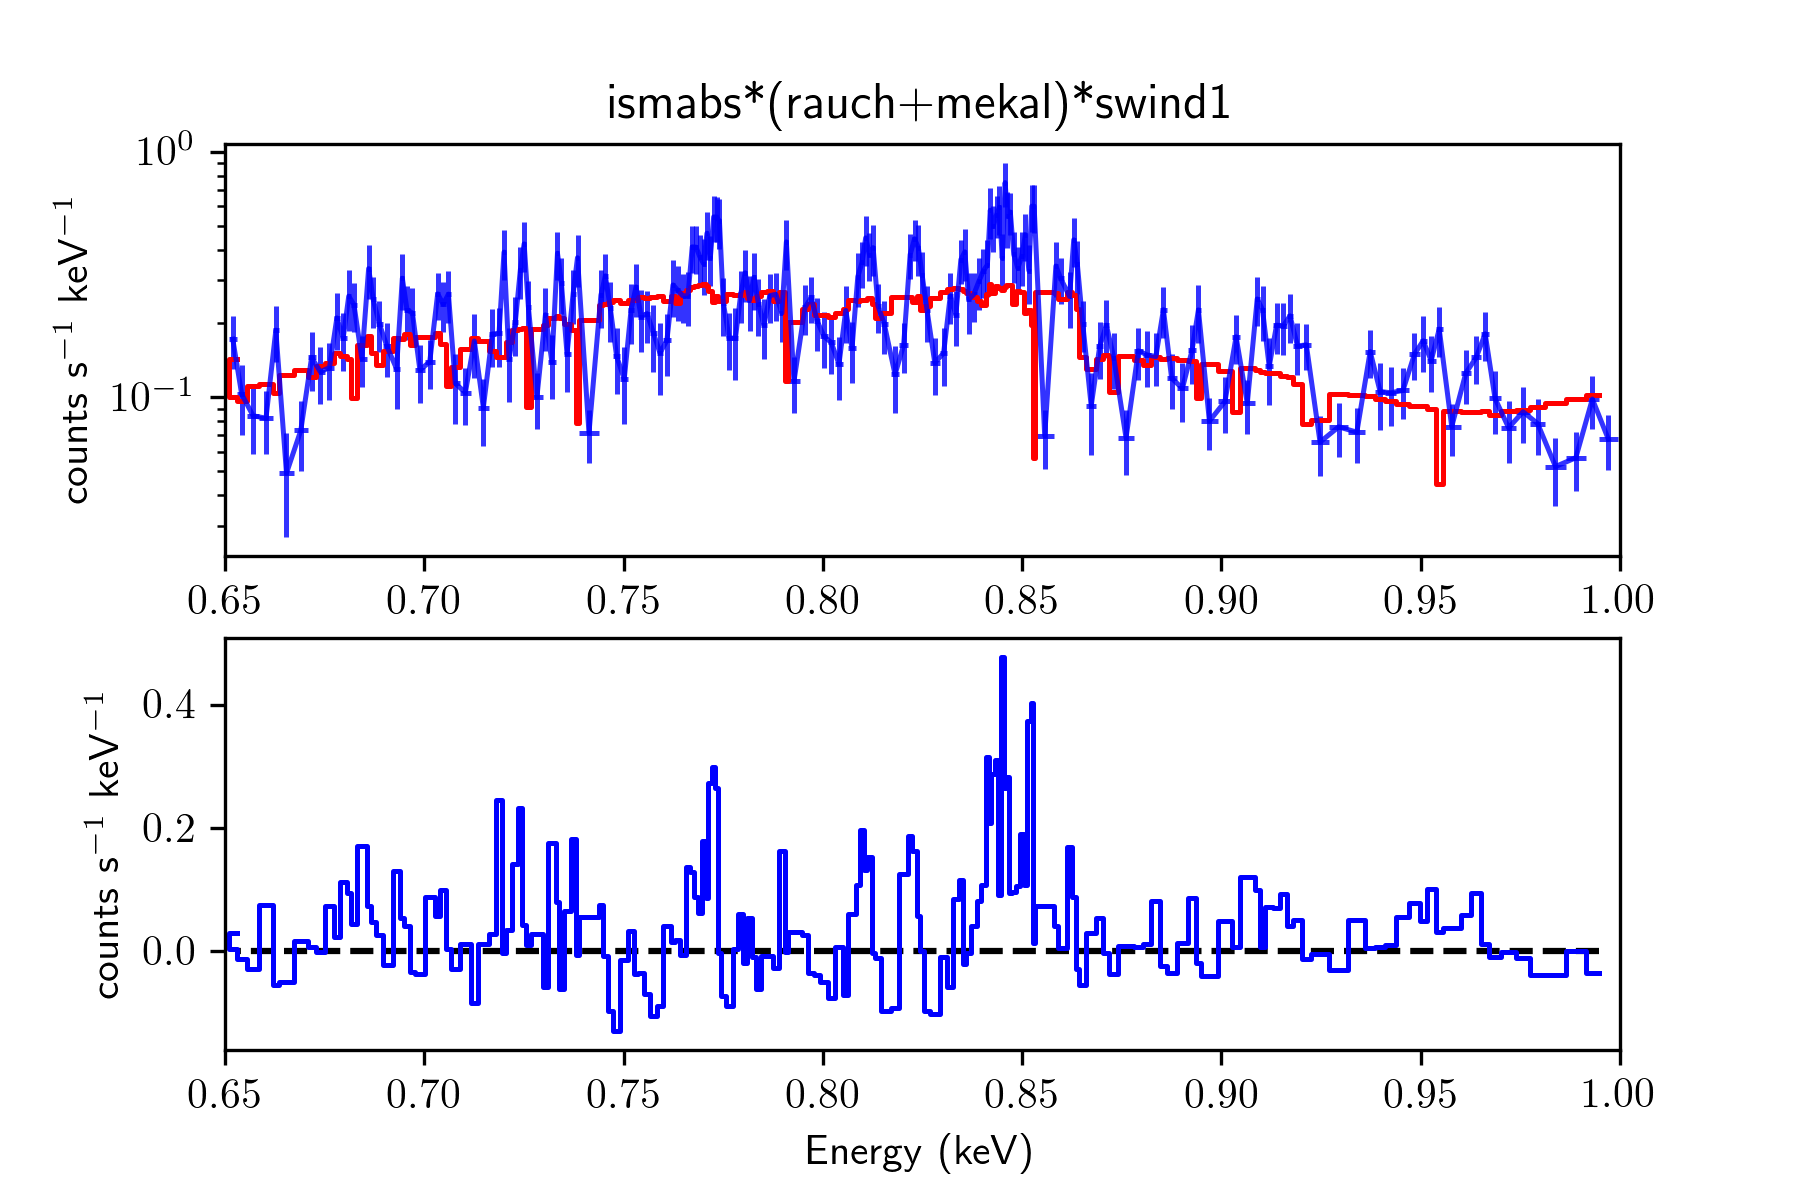
\includegraphics[width=0.45\textwidth]{mrvel-rgs1-o2-m09}} %\hfill
			\end{figure}
			\begin{figure}[h!]
				\centering
				\caption{Spectral fits for RGS1 spectra using model M10}
				\label{xmm:rgs1-m10}
				\subfloat[Order 1 \label{xmm:rgs1-m10:o1}]{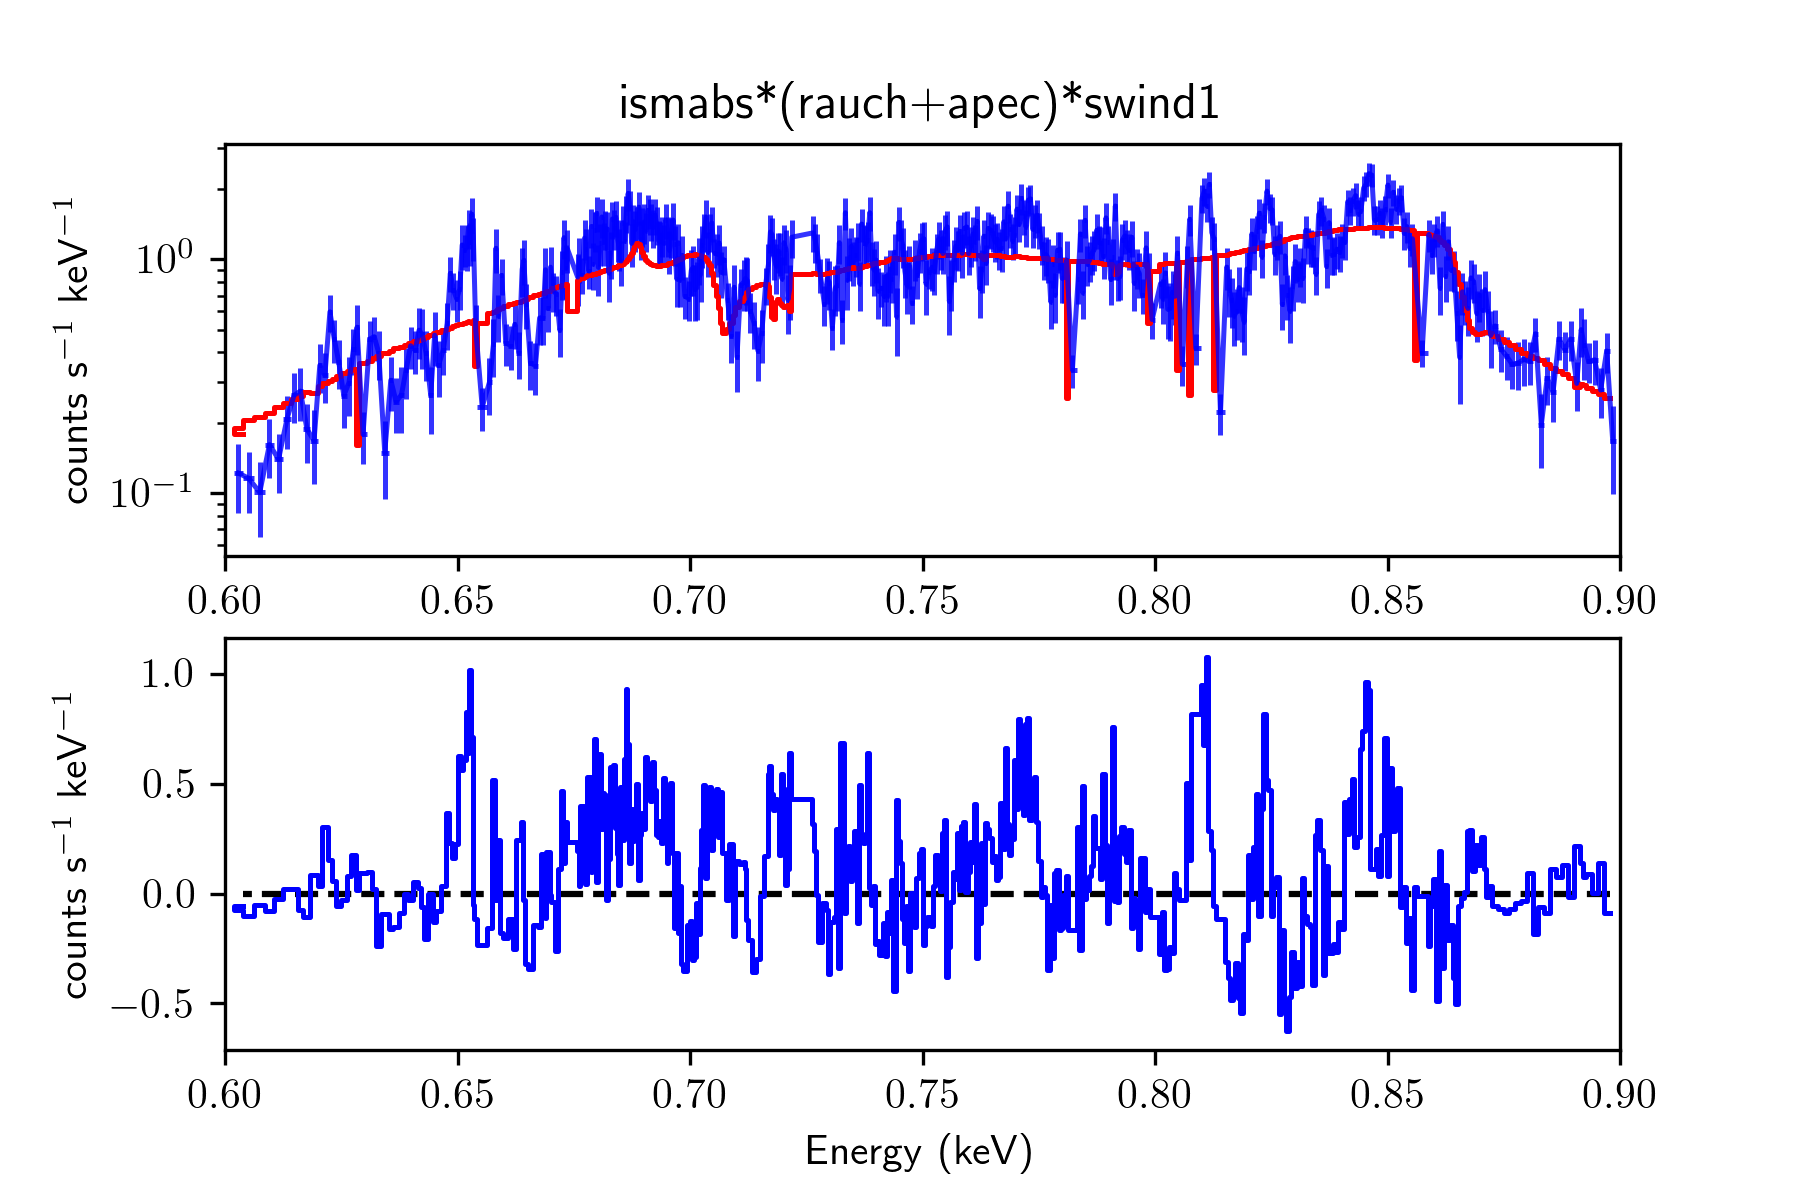
\includegraphics[width=0.45\textwidth]{mrvel-rgs1-o1-m10}} %\hfill
				\subfloat[Order 2 \label{xmm:rgs1-m10:o2}]{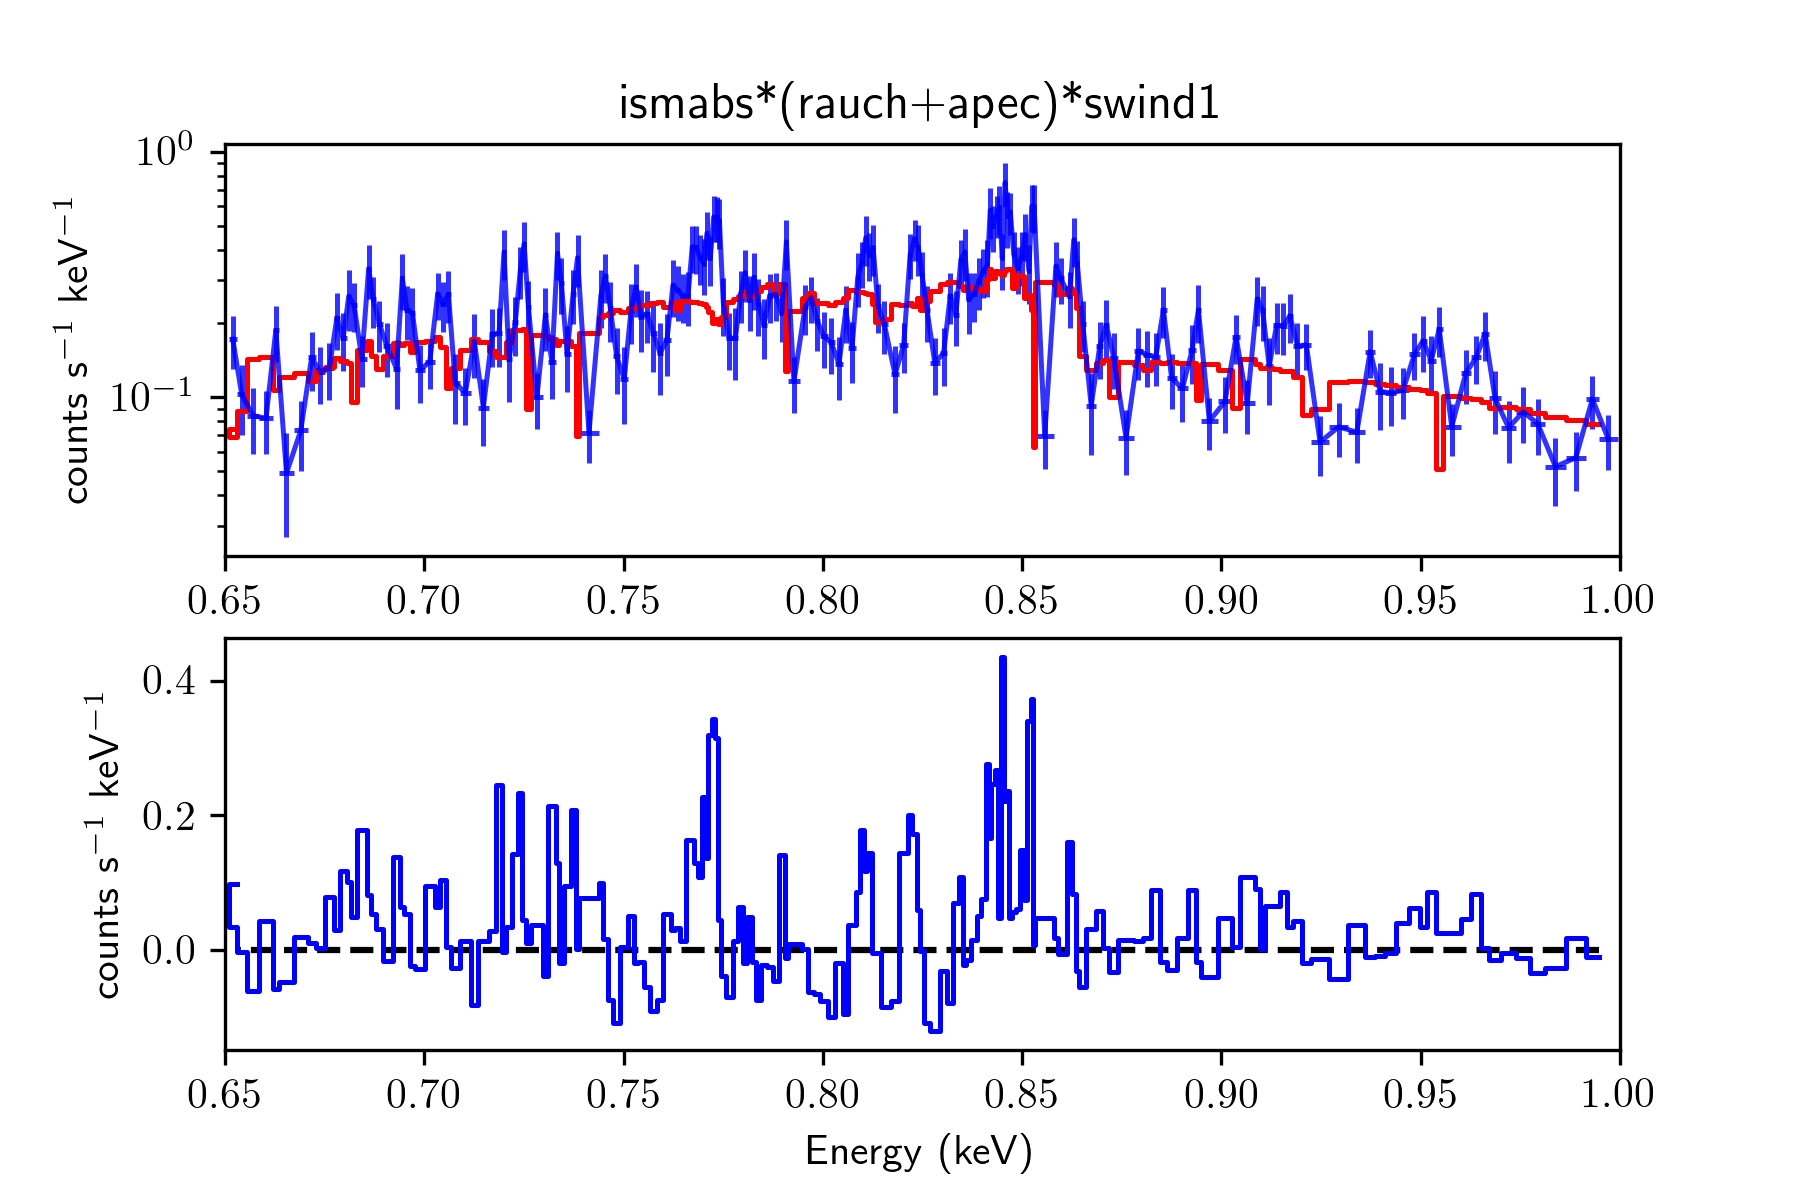
\includegraphics[width=0.45\textwidth]{mrvel-rgs1-o2-m10}} %\hfill
			\end{figure}
			\begin{figure}[h!]
				\centering
				\caption{Spectral fits for RGS1 spectra using model M11}
				\label{xmm:rgs1-m11}
				\subfloat[Order 1 \label{xmm:rgs1-m11:o1}]{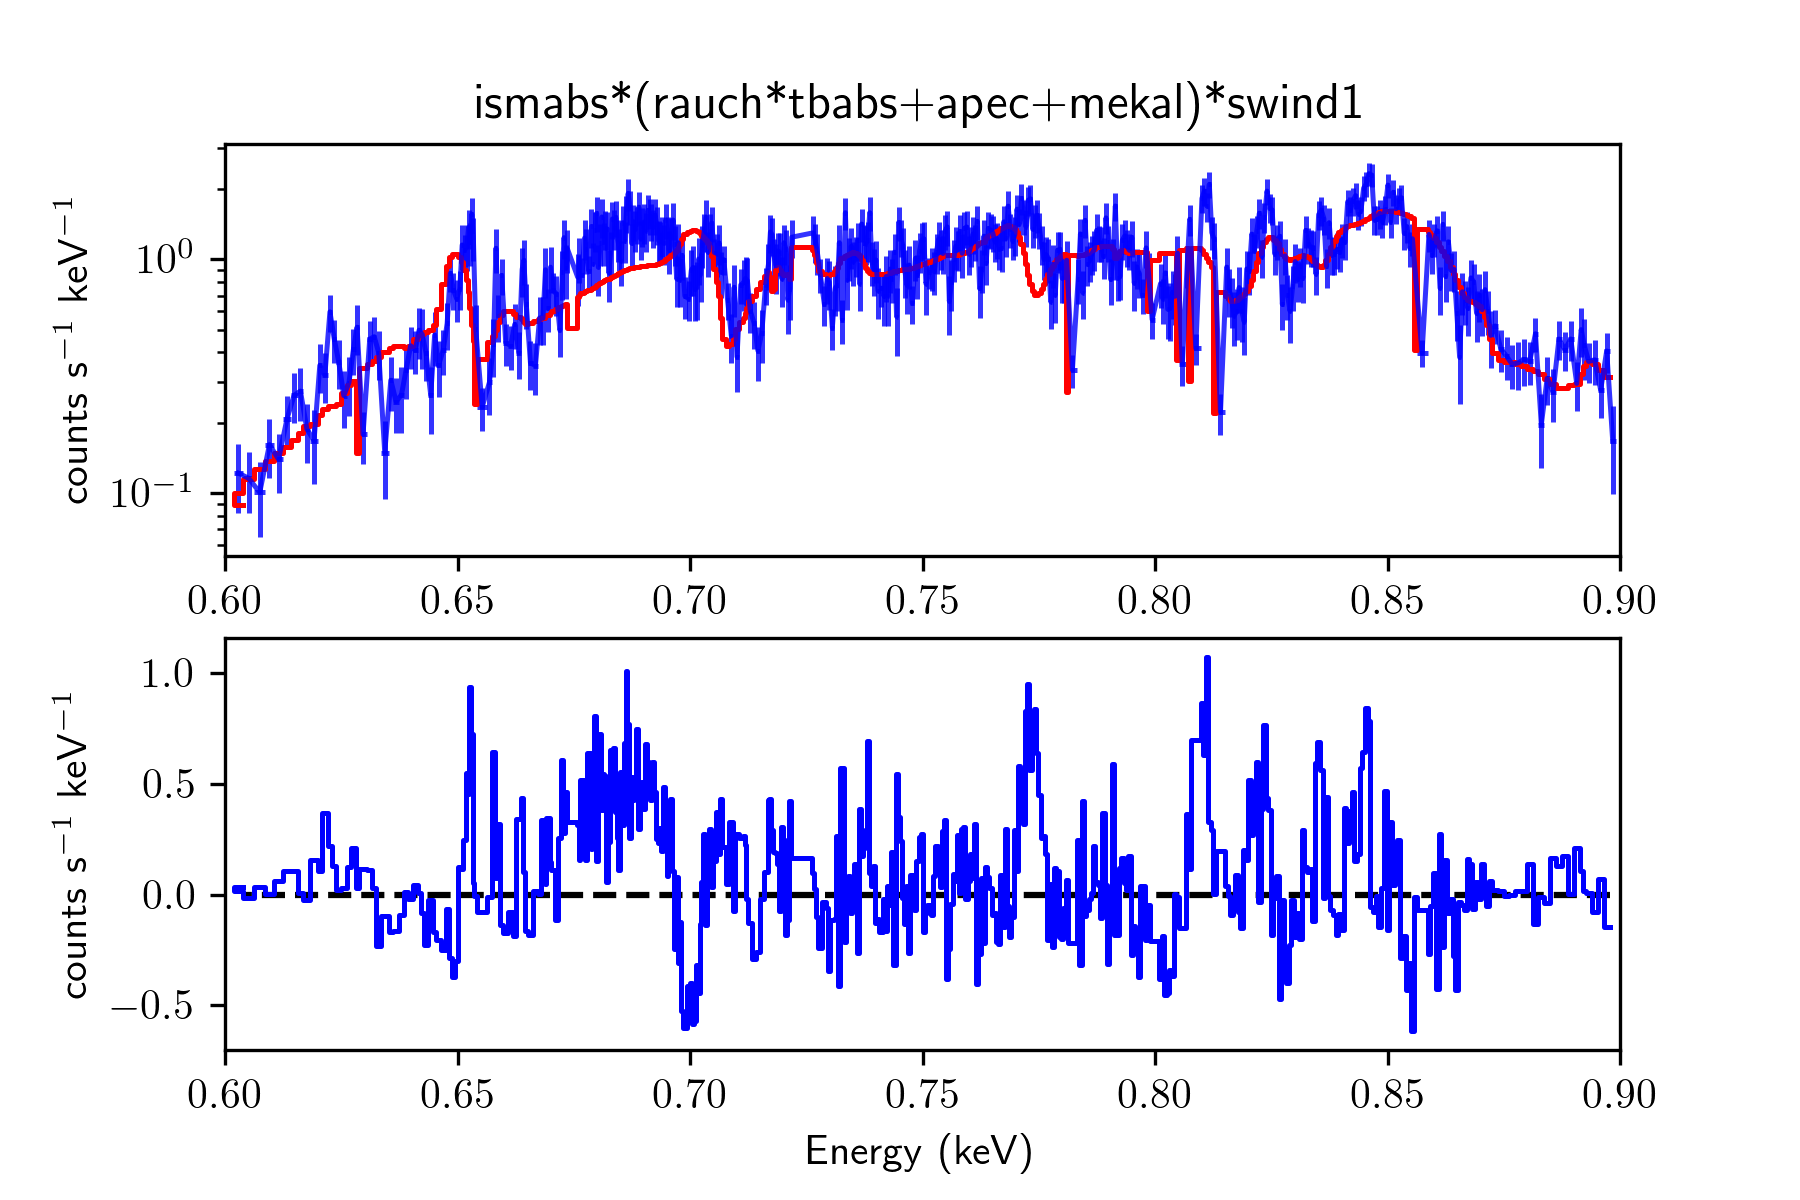
\includegraphics[width=0.45\textwidth]{mrvel-rgs1-o1-m11}} %\hfill
				\subfloat[Order 2 \label{xmm:rgs1-m11:o2}]{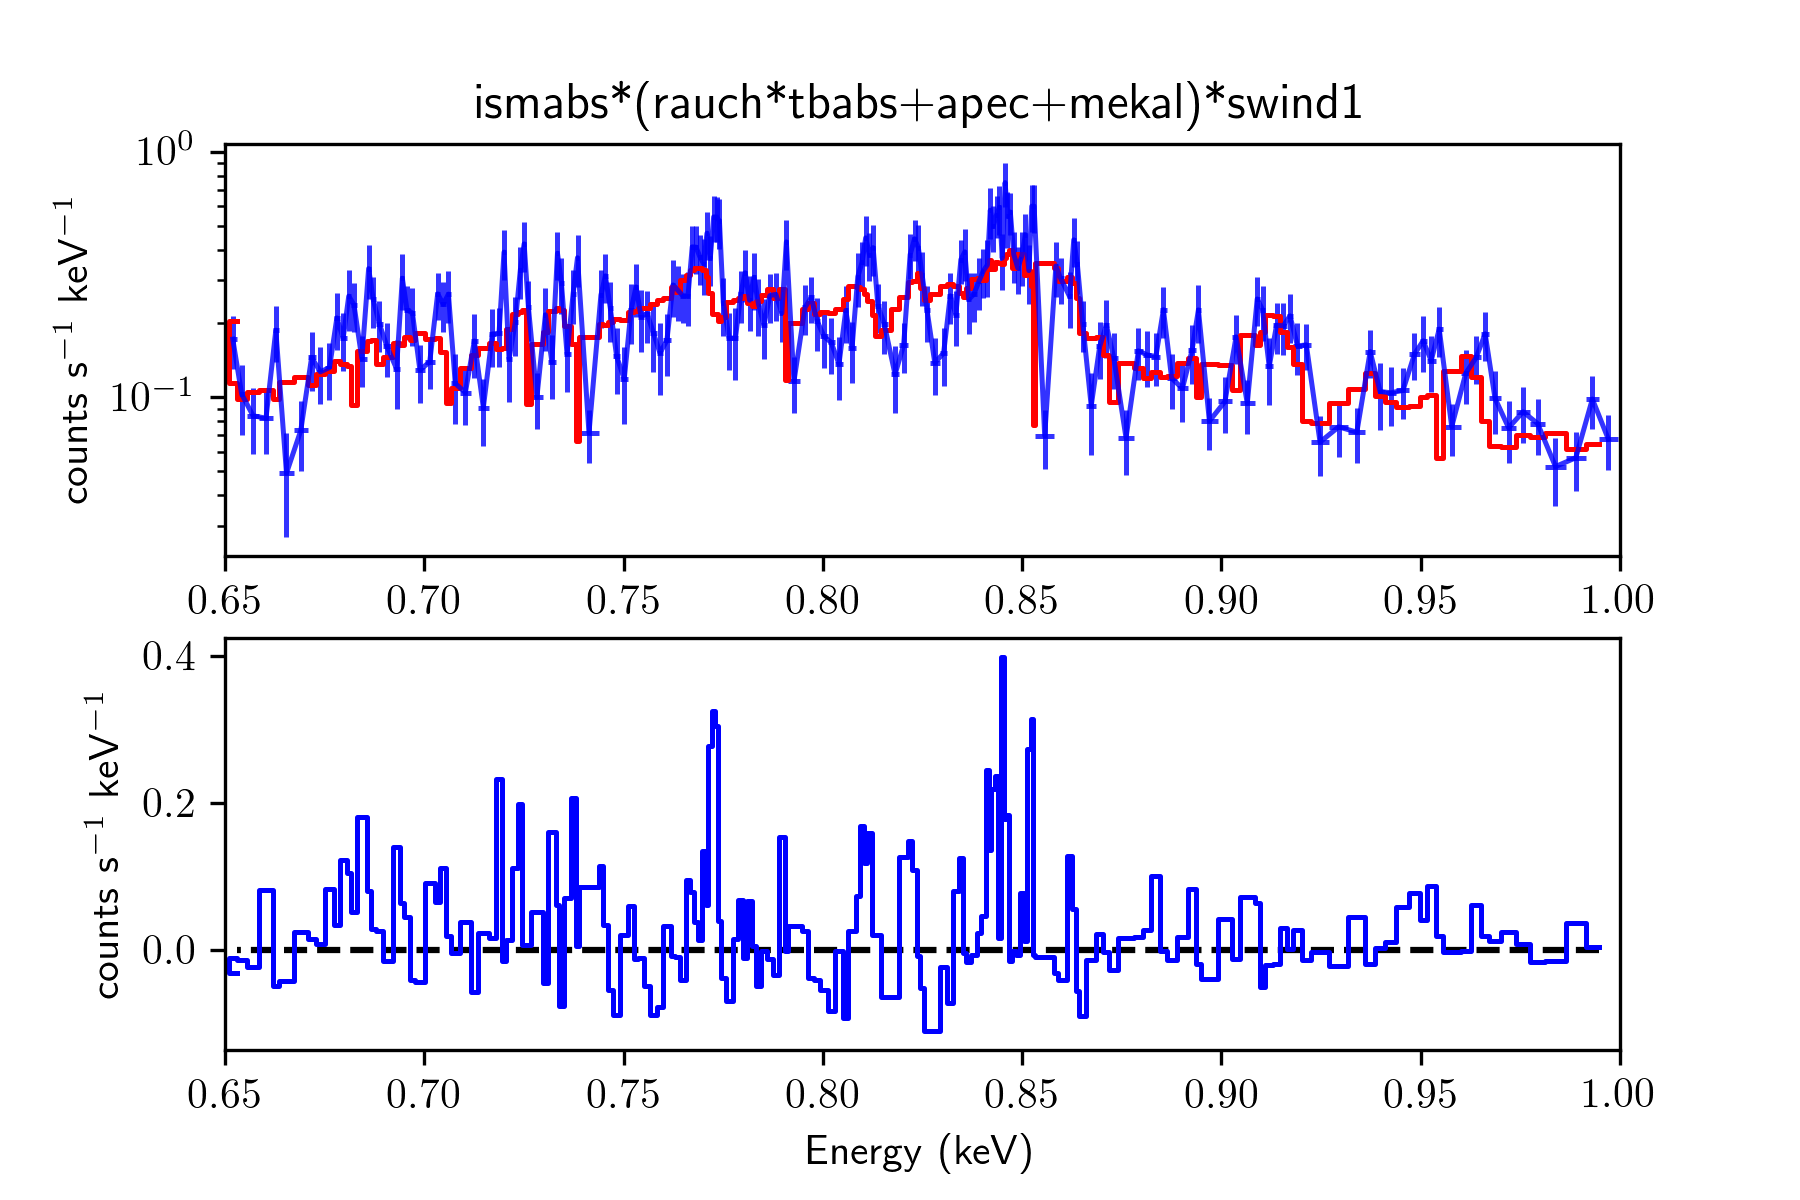
\includegraphics[width=0.45\textwidth]{mrvel-rgs1-o2-m11}} %\hfill
			\end{figure}
			\begin{figure}[h!]
				\centering
				\caption{Spectral fits for RGS1 spectra using model M12}
				\label{xmm:rgs1-m12}
				\subfloat[Order 1 \label{xmm:rgs1-m12:o1}]{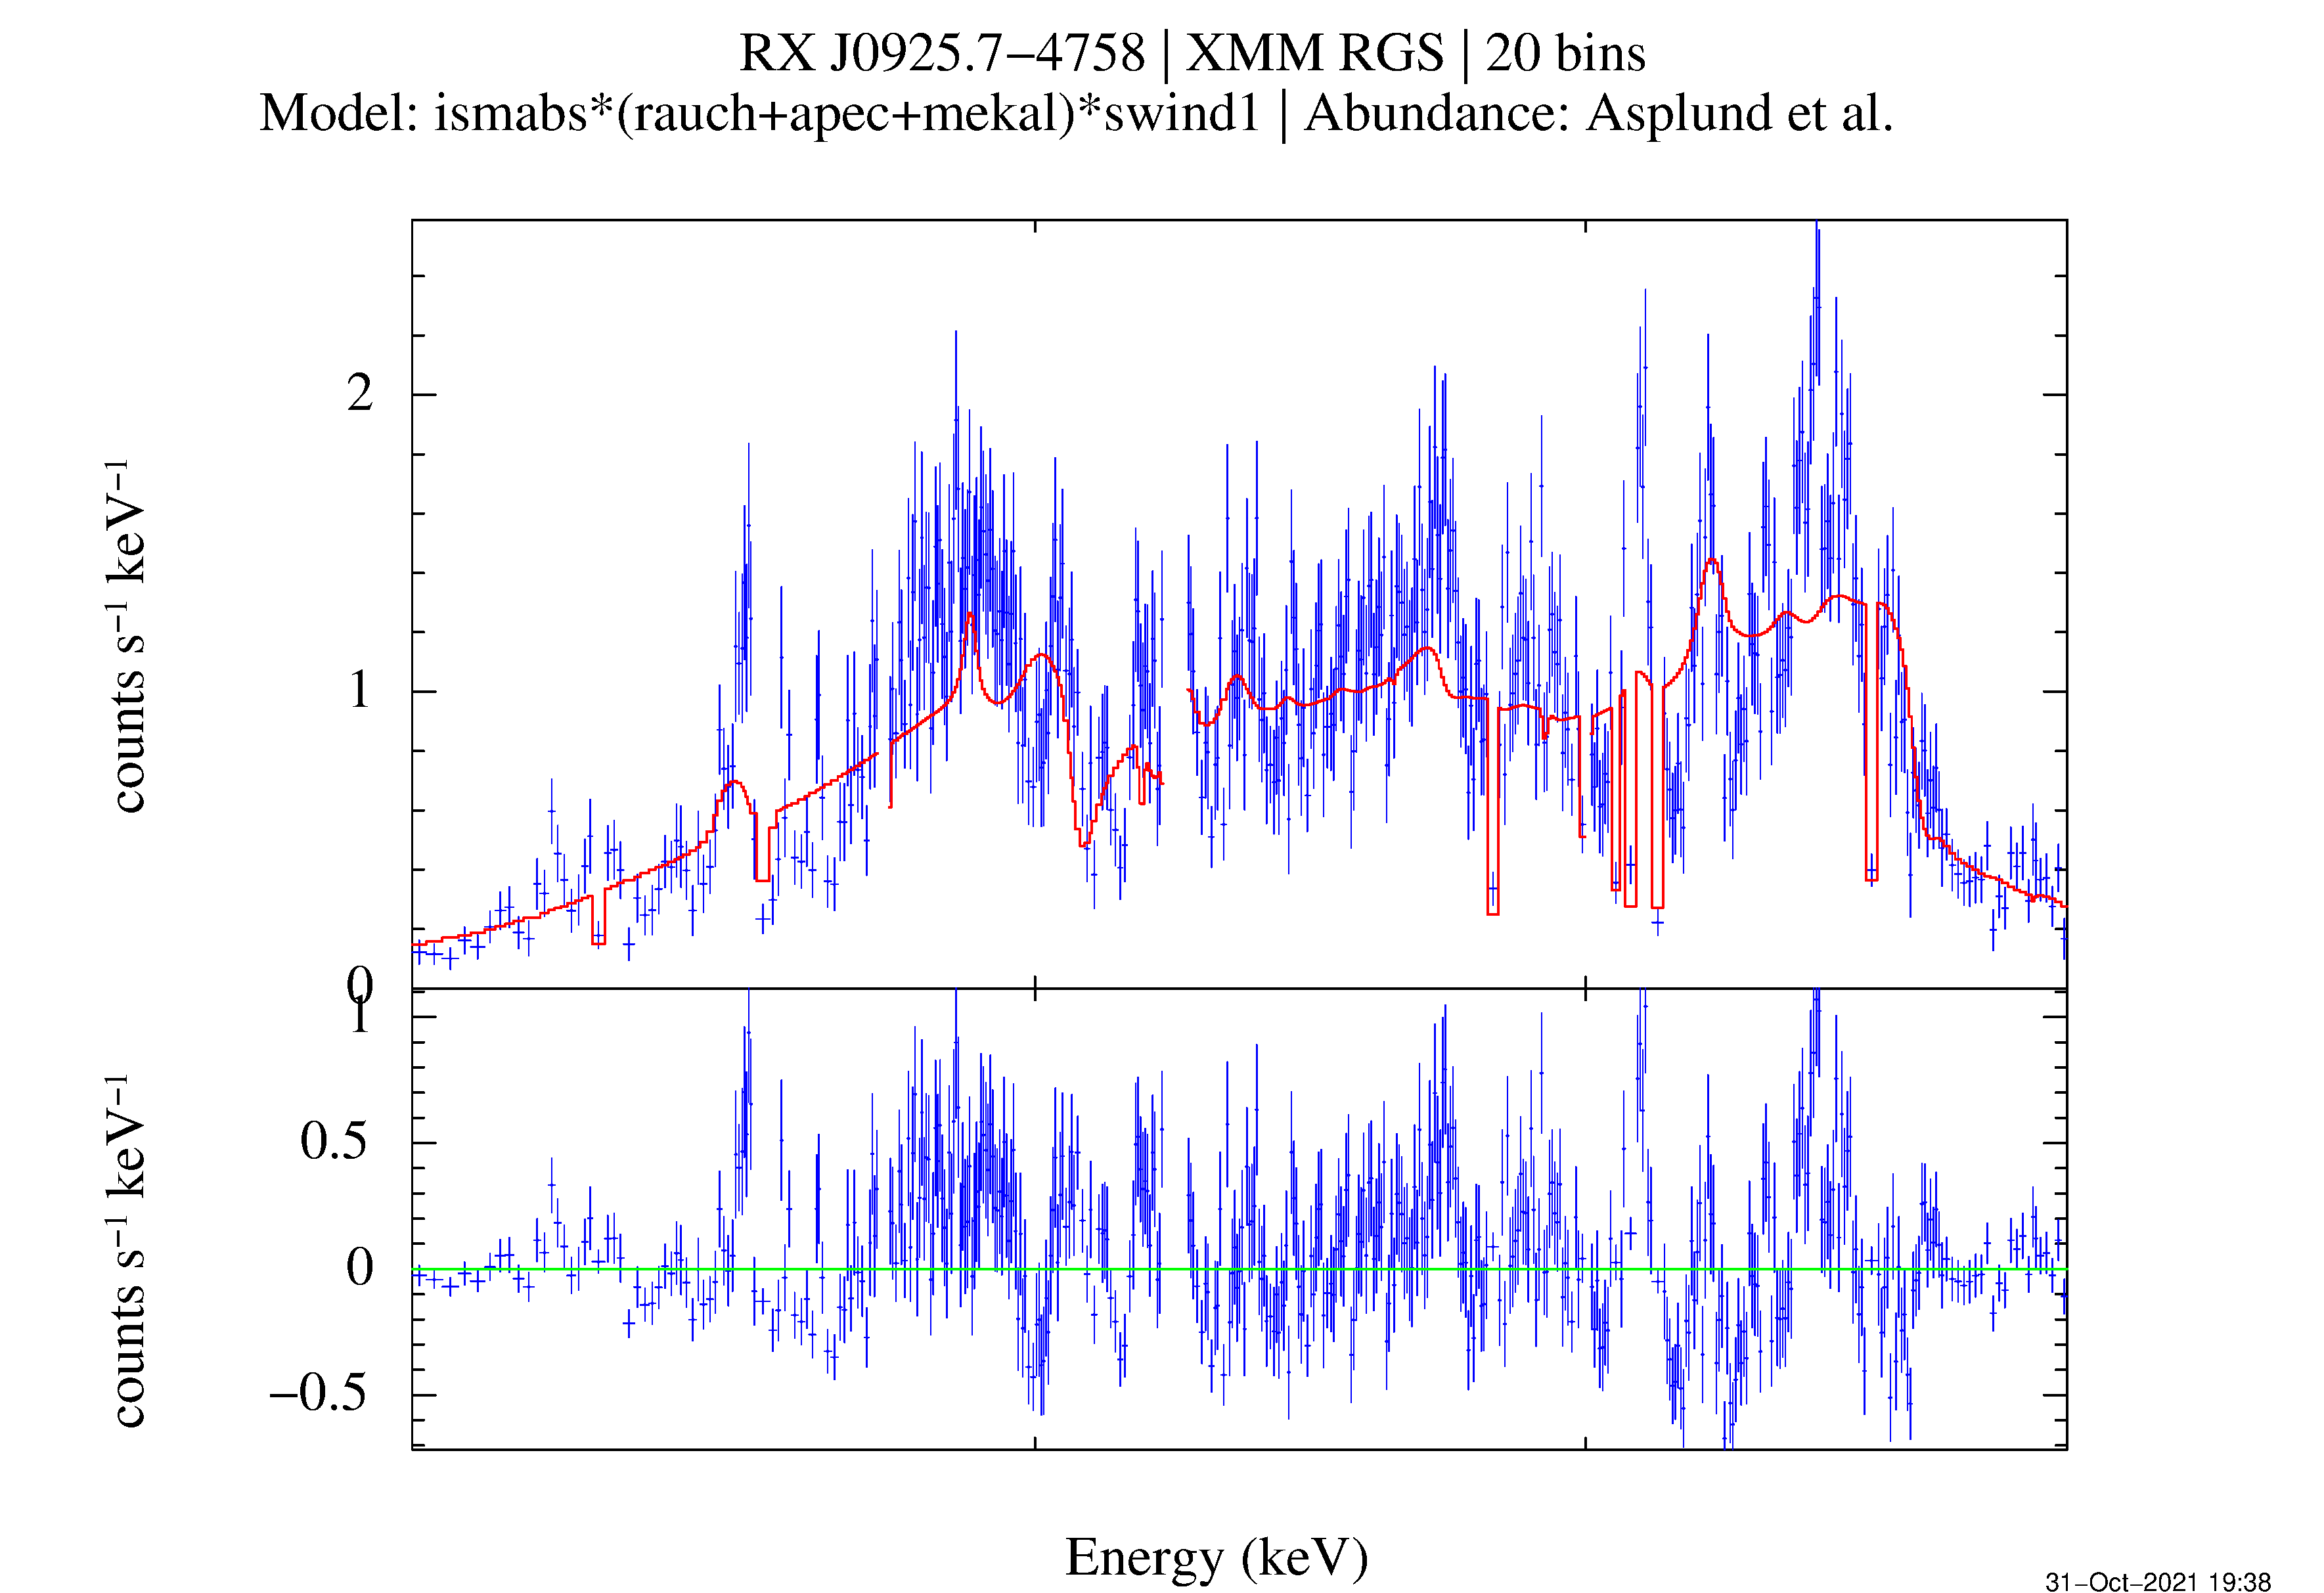
\includegraphics[width=0.45\textwidth]{mrvel-rgs1-o1-m12}} %\hfill
				\subfloat[Order 2 \label{xmm:rgs1-m12:o2}]{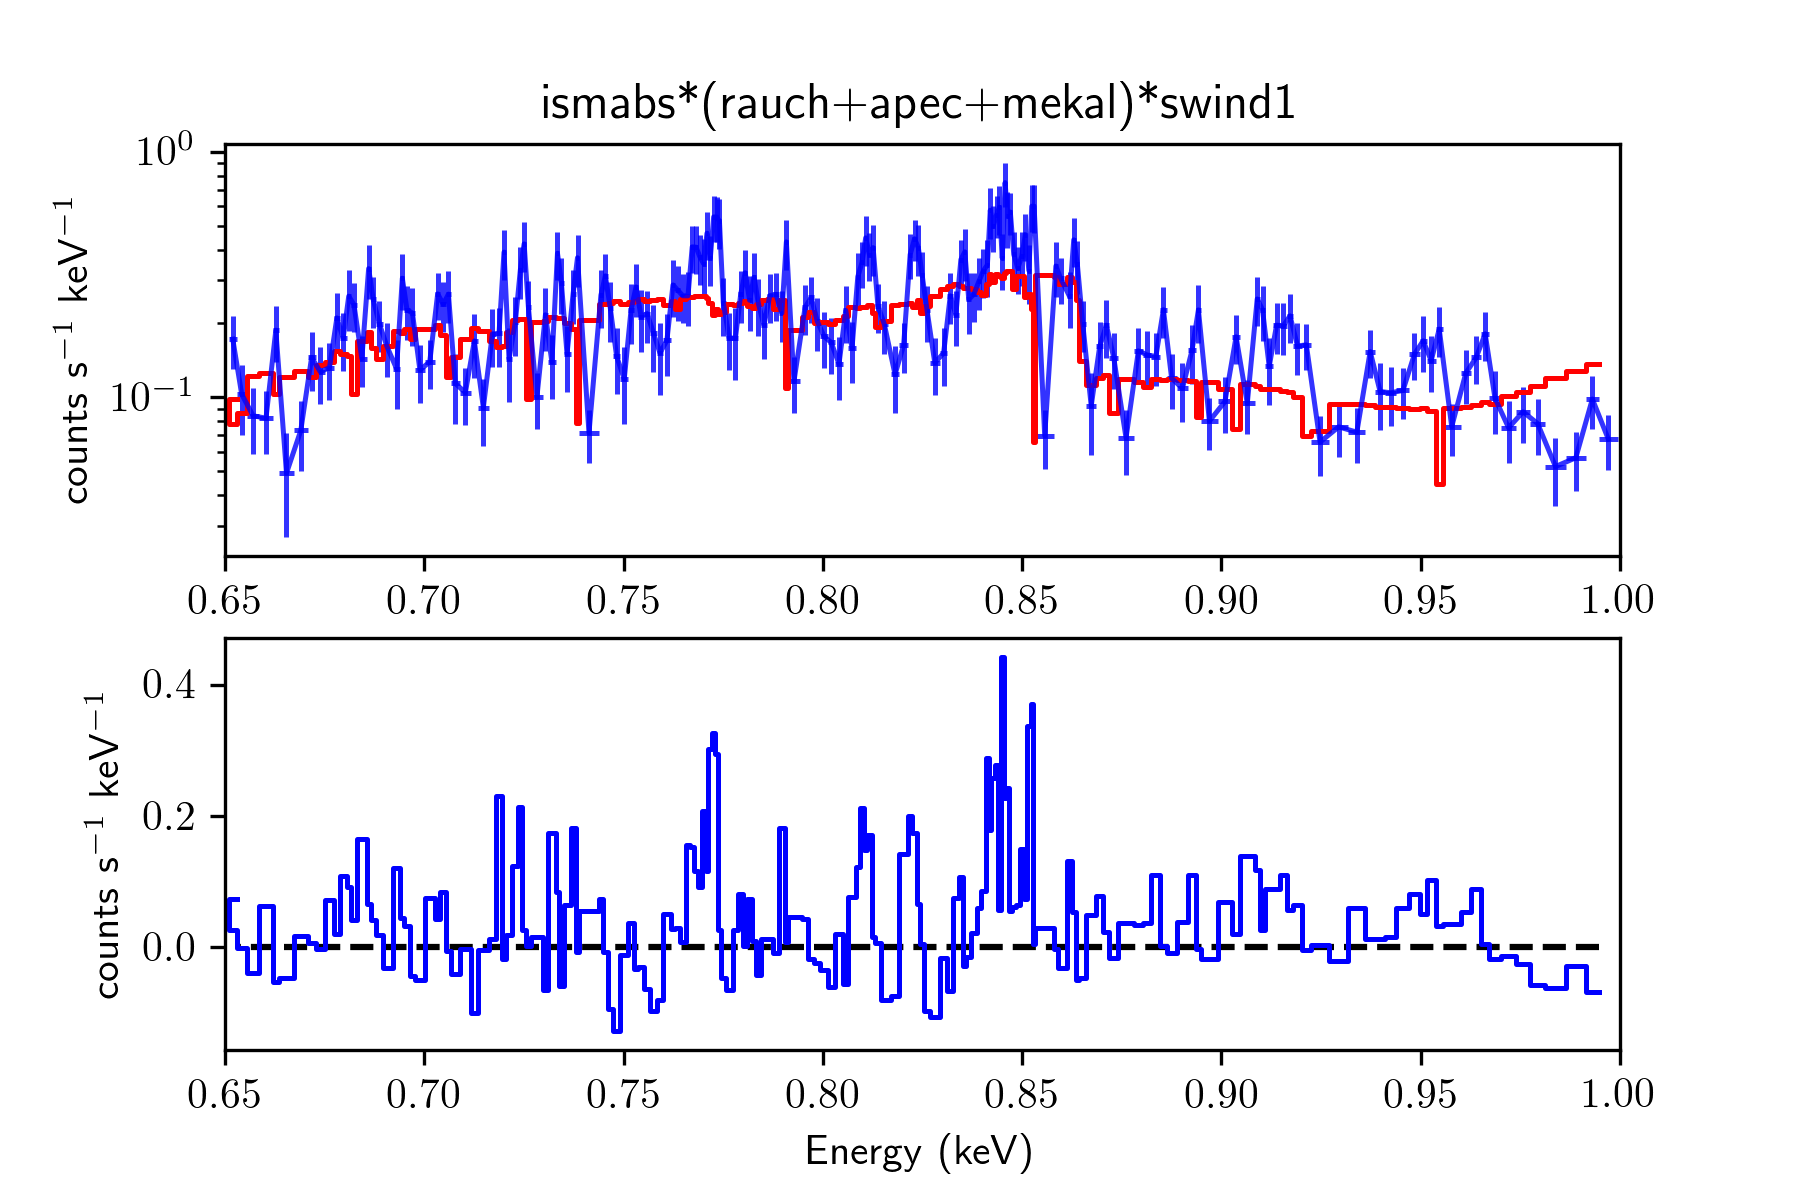
\includegraphics[width=0.45\textwidth]{mrvel-rgs1-o2-m12}} %\hfill
			\end{figure}
		
		\clearpage
		\subsection{Fitting of RGS2 Spectra} \label{hi-resolution:analysis:rgs2}
			Here as well the best fits for both diffraction orders were obtained using the model M11. This seems to suggest that model M11 might be the best candidate model for RX J0925.7-4758. All the other models yield $\chi^2_\text{red}$ to be outside the acceptable range, with the exception of the model M08, which lies almost on the borderline. The trend shown by the $\chi^2_\text{red}$ across all the models considered here are shown in figure \ref{fig:mrvel-rgs2-chisq}.
			
			\begin{figure}[h!]
				\centering
				\caption{$\chi^2_\text{red}$ trend for RX J0925.7-4758 spectra from RGS2 instrument}
				\label{fig:mrvel-rgs2-chisq}
				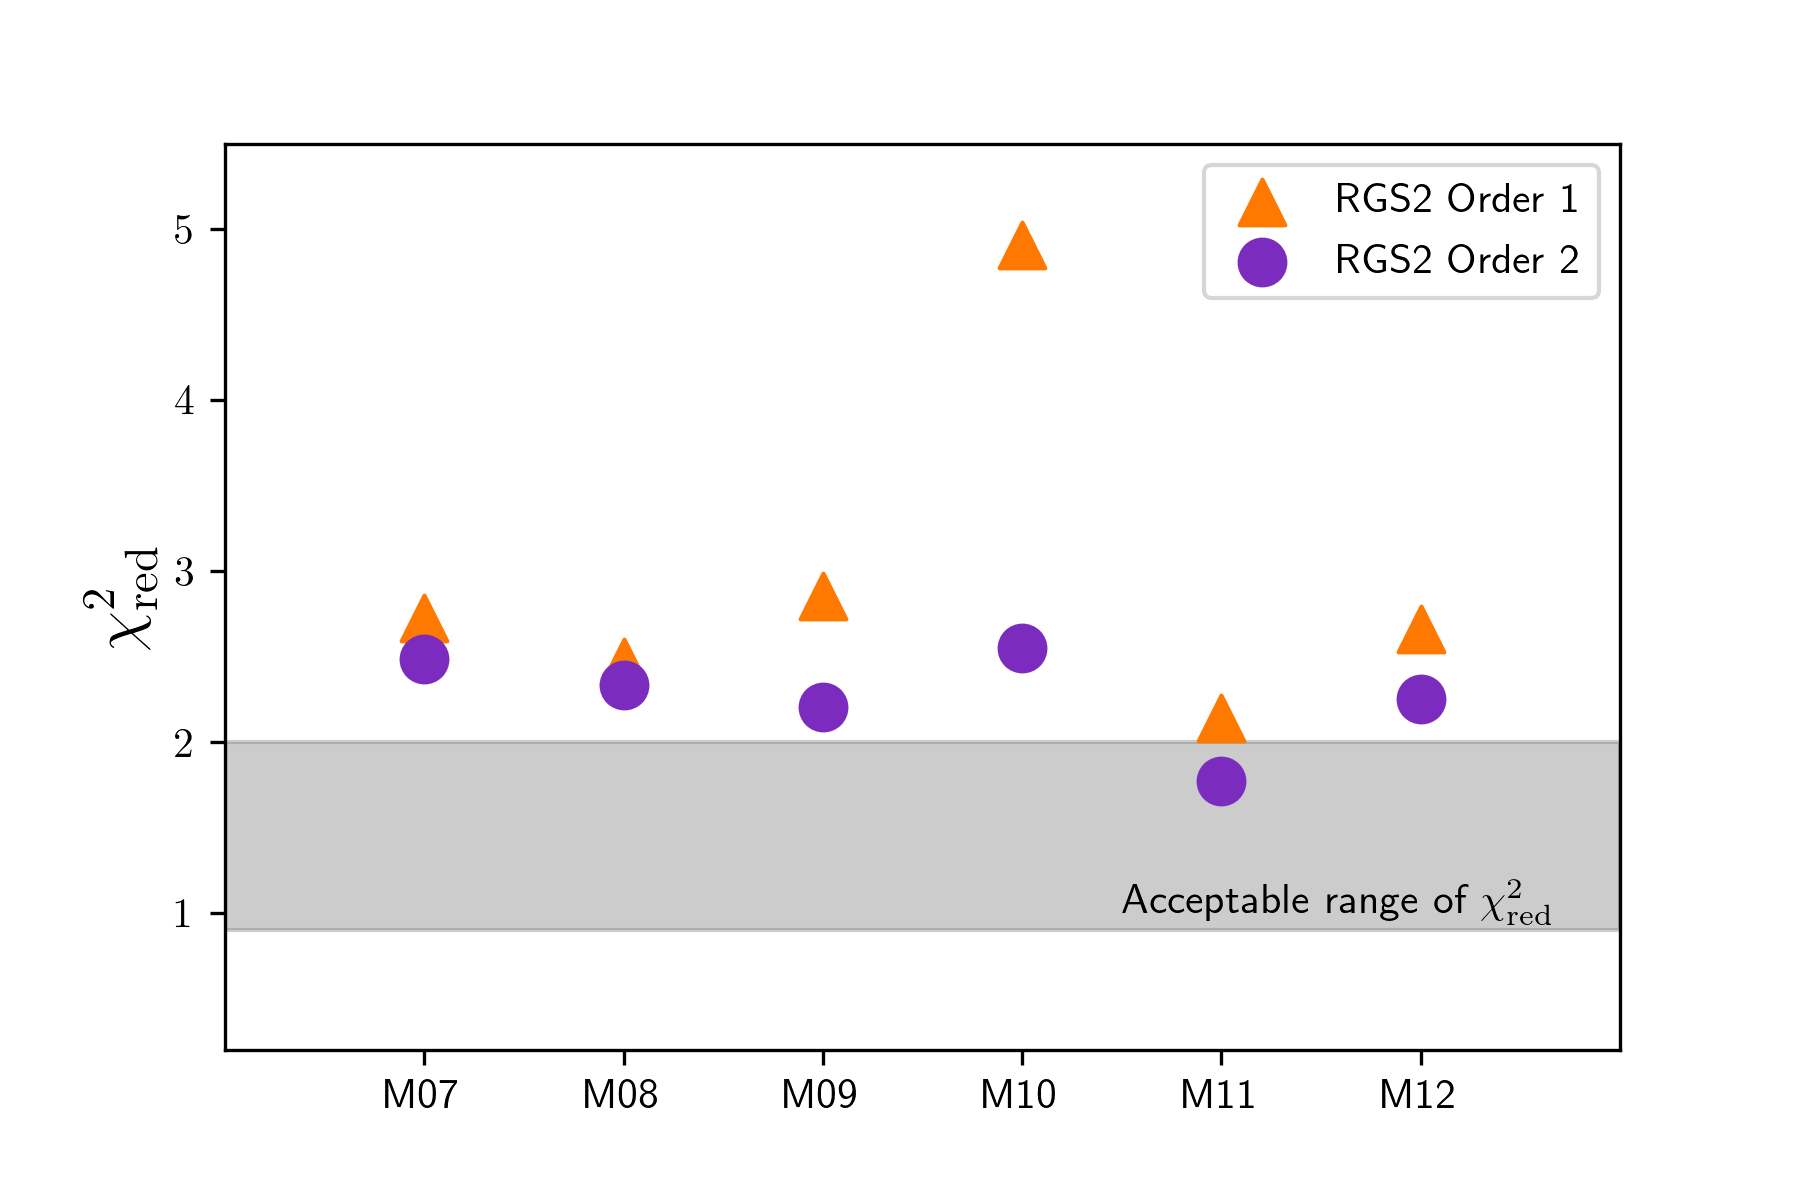
\includegraphics[width=0.85\textwidth]{mrvel-rgs2-chisq}
			\end{figure}
			The fitted spectra, along with the residuals are displayed as follows:
			\begin{figure}[h!]
				\centering
				\caption{Spectral fits for RGS2 spectra using model M07}
				\label{xmm:rgs2-m07}
				\subfloat[Order 1 \label{xmm:rgs2-m07:o1}]{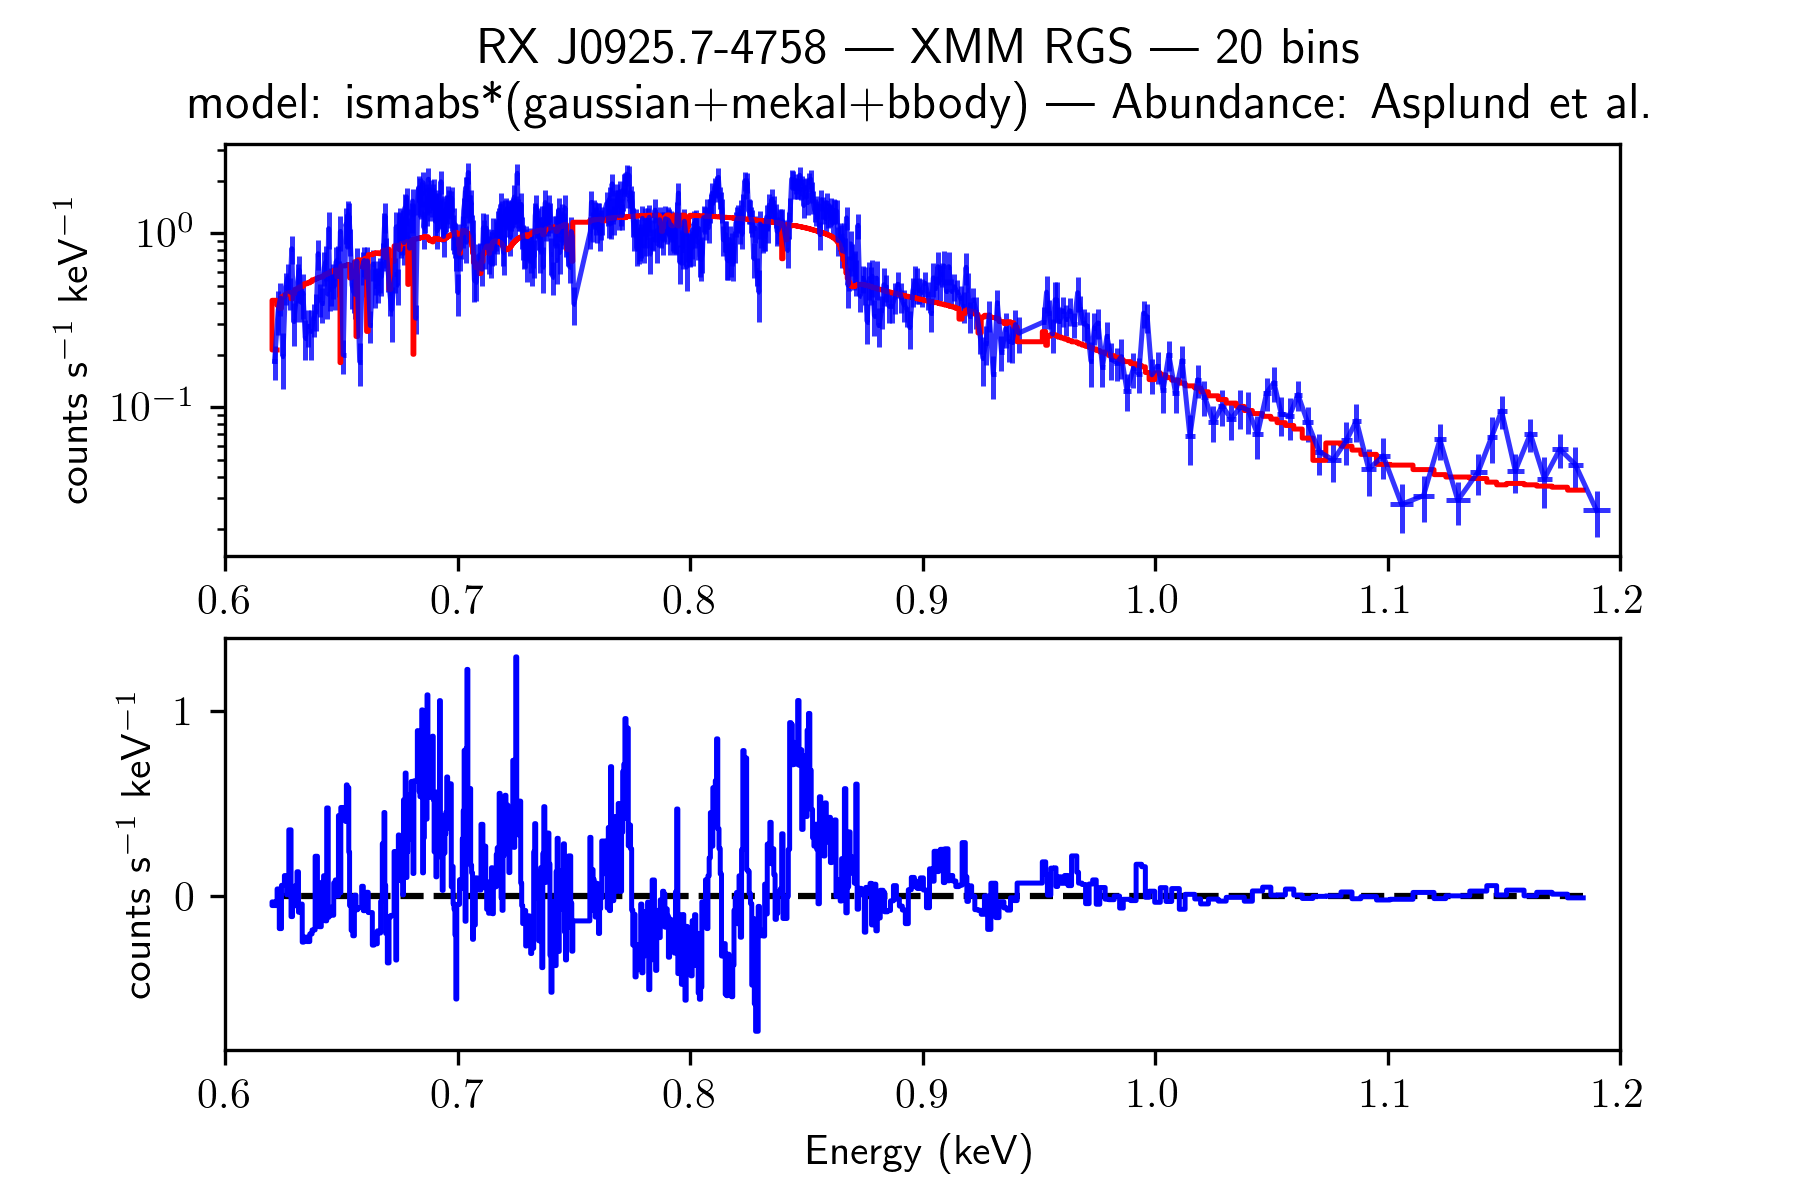
\includegraphics[width=0.45\textwidth]{mrvel-rgs2-o1-m07}} %\hfill
				\subfloat[Order 2 \label{xmm:rgs2-m07:o2}]{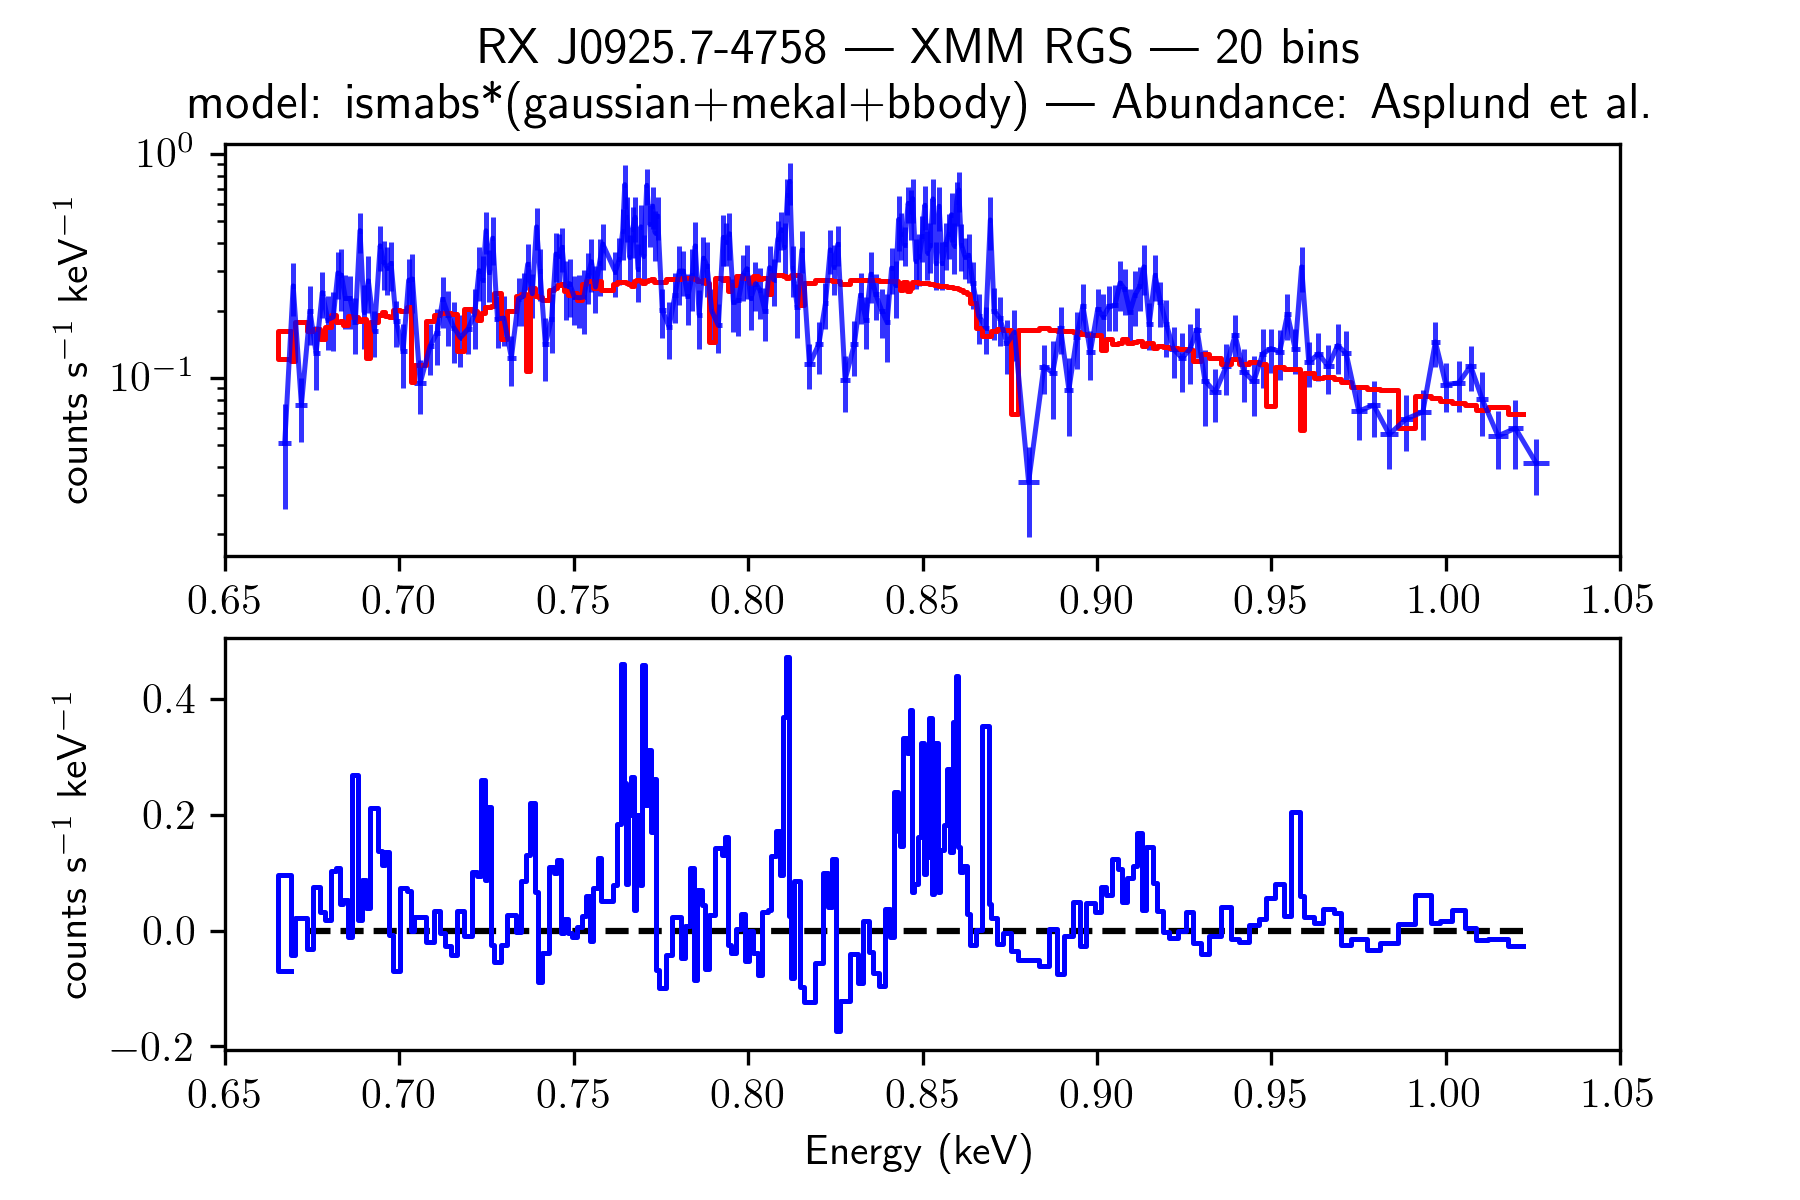
\includegraphics[width=0.45\textwidth]{mrvel-rgs2-o2-m07}} %\hfill
			\end{figure}
			\begin{figure}[h!]
				\centering
				\caption{Spectral fits for RGS2 spectra using model M08}
				\label{xmm:rgs2-m08}
				\subfloat[Order 1 \label{xmm:rgs2-m08:o1}]{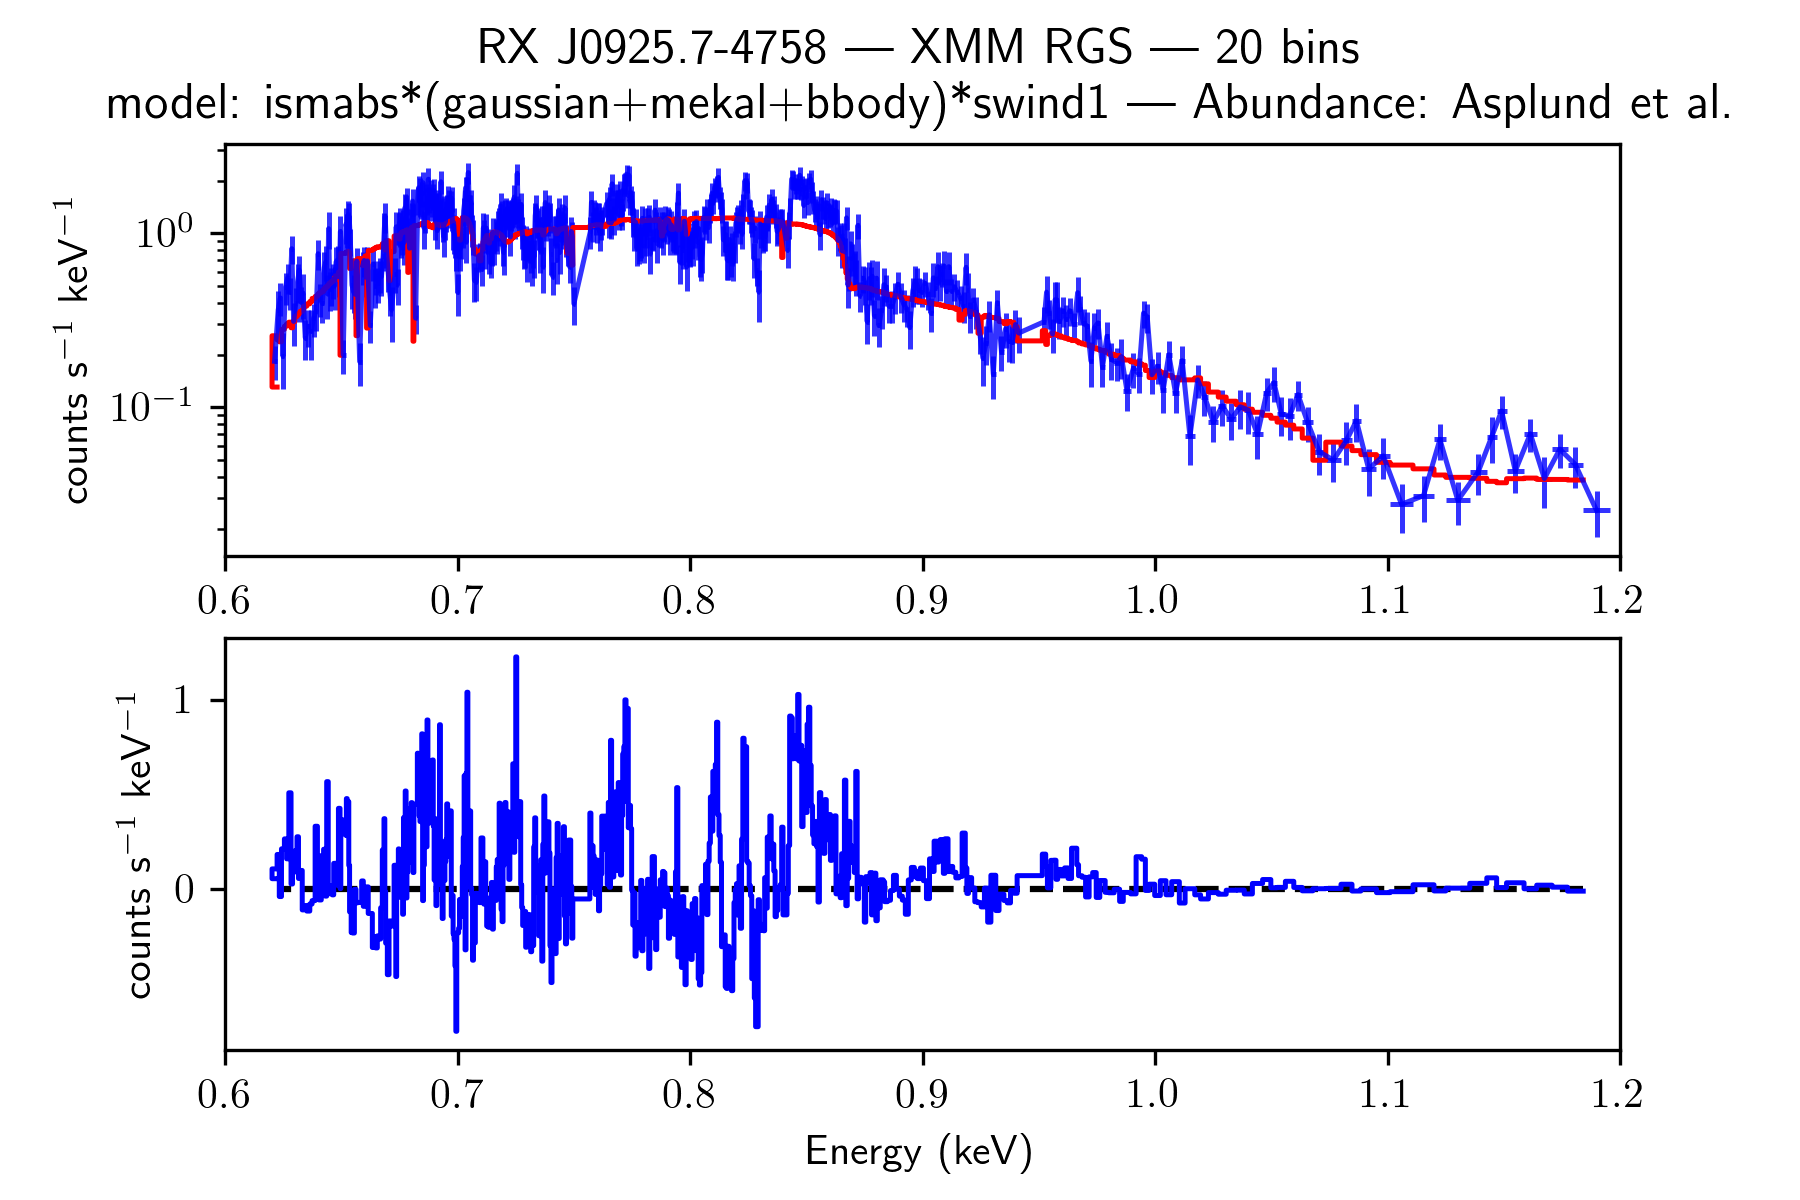
\includegraphics[width=0.45\textwidth]{mrvel-rgs2-o1-m08}} %\hfill
				\subfloat[Order 2 \label{xmm:rgs2-m08:o2}]{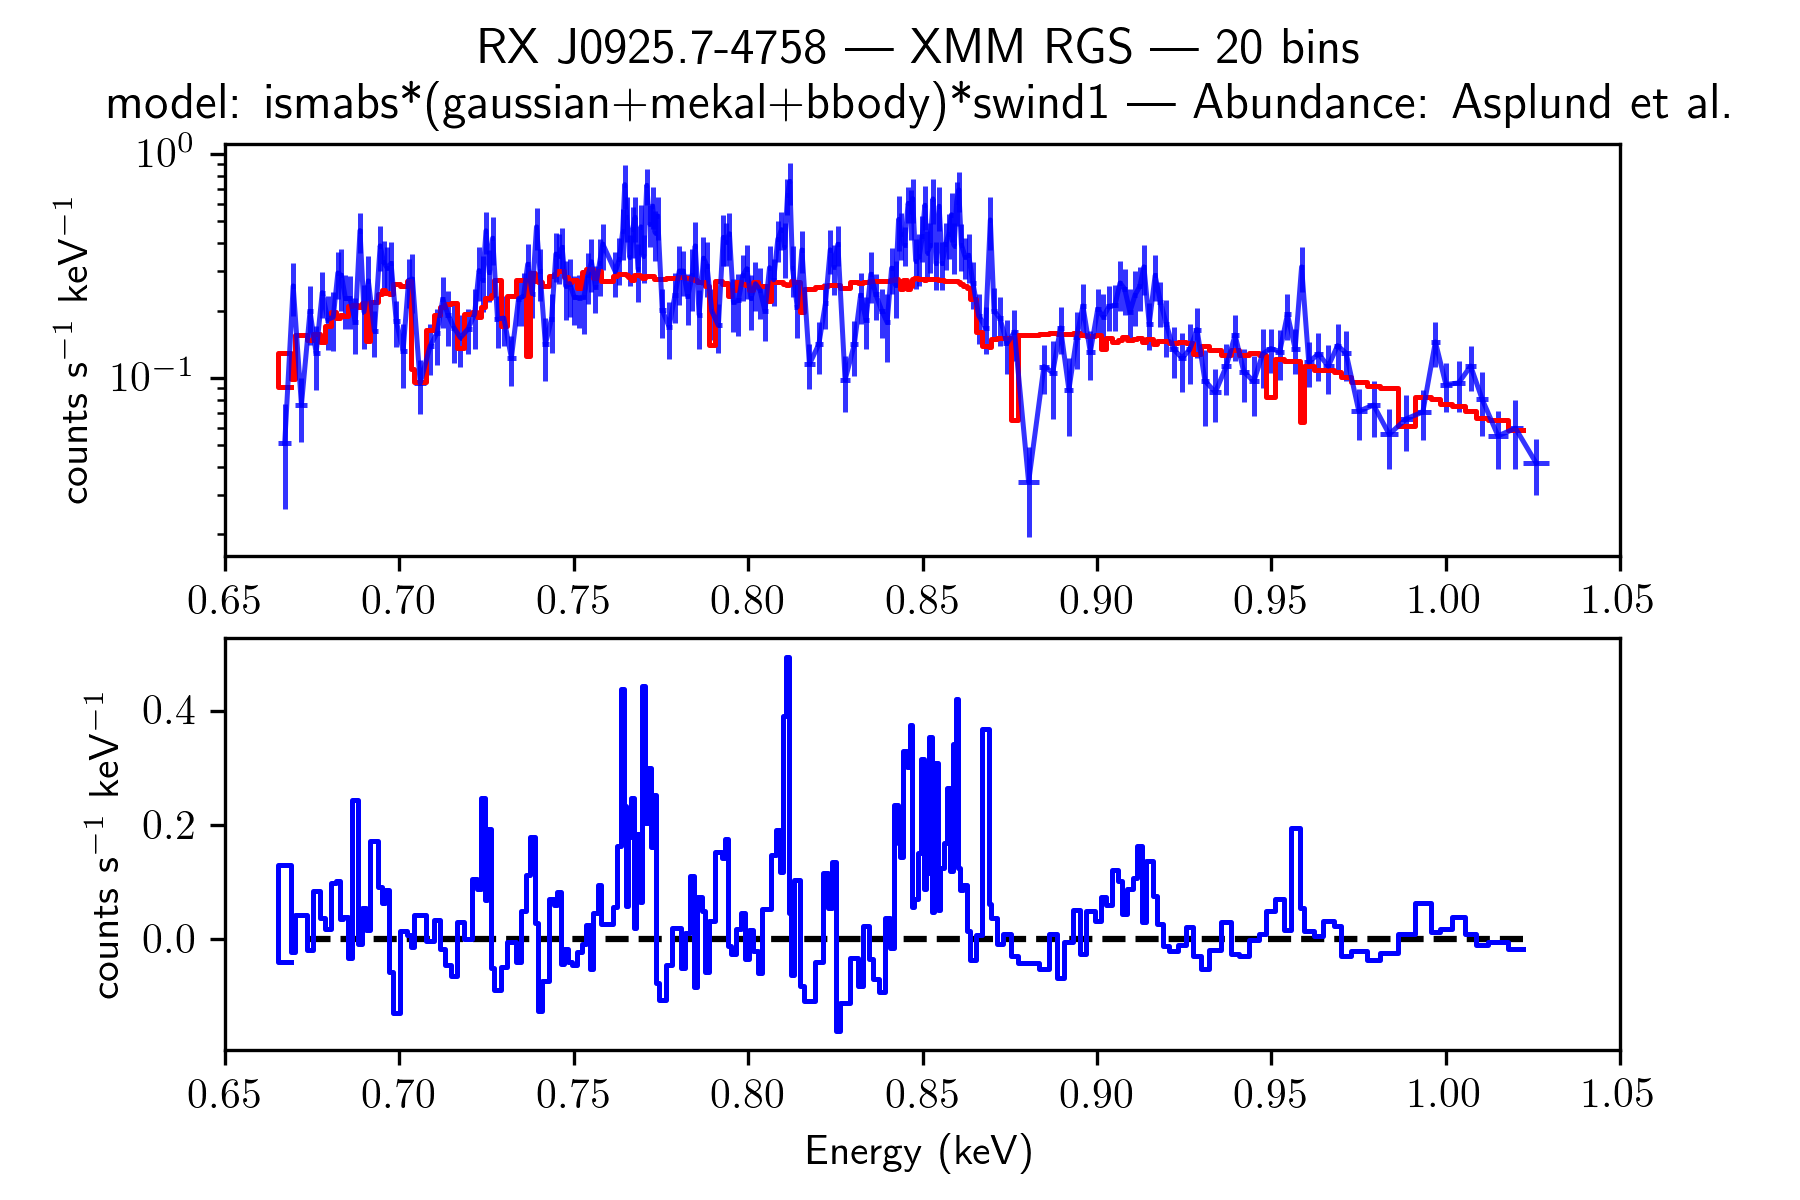
\includegraphics[width=0.45\textwidth]{mrvel-rgs2-o2-m08}} %\hfill
			\end{figure}
			\begin{figure}[h!]
				\centering
				\caption{Spectral fits for RGS2 spectra using model M09}
				\label{xmm:rgs2-m09}
				\subfloat[Order 1 \label{xmm:rgs2-m09:o1}]{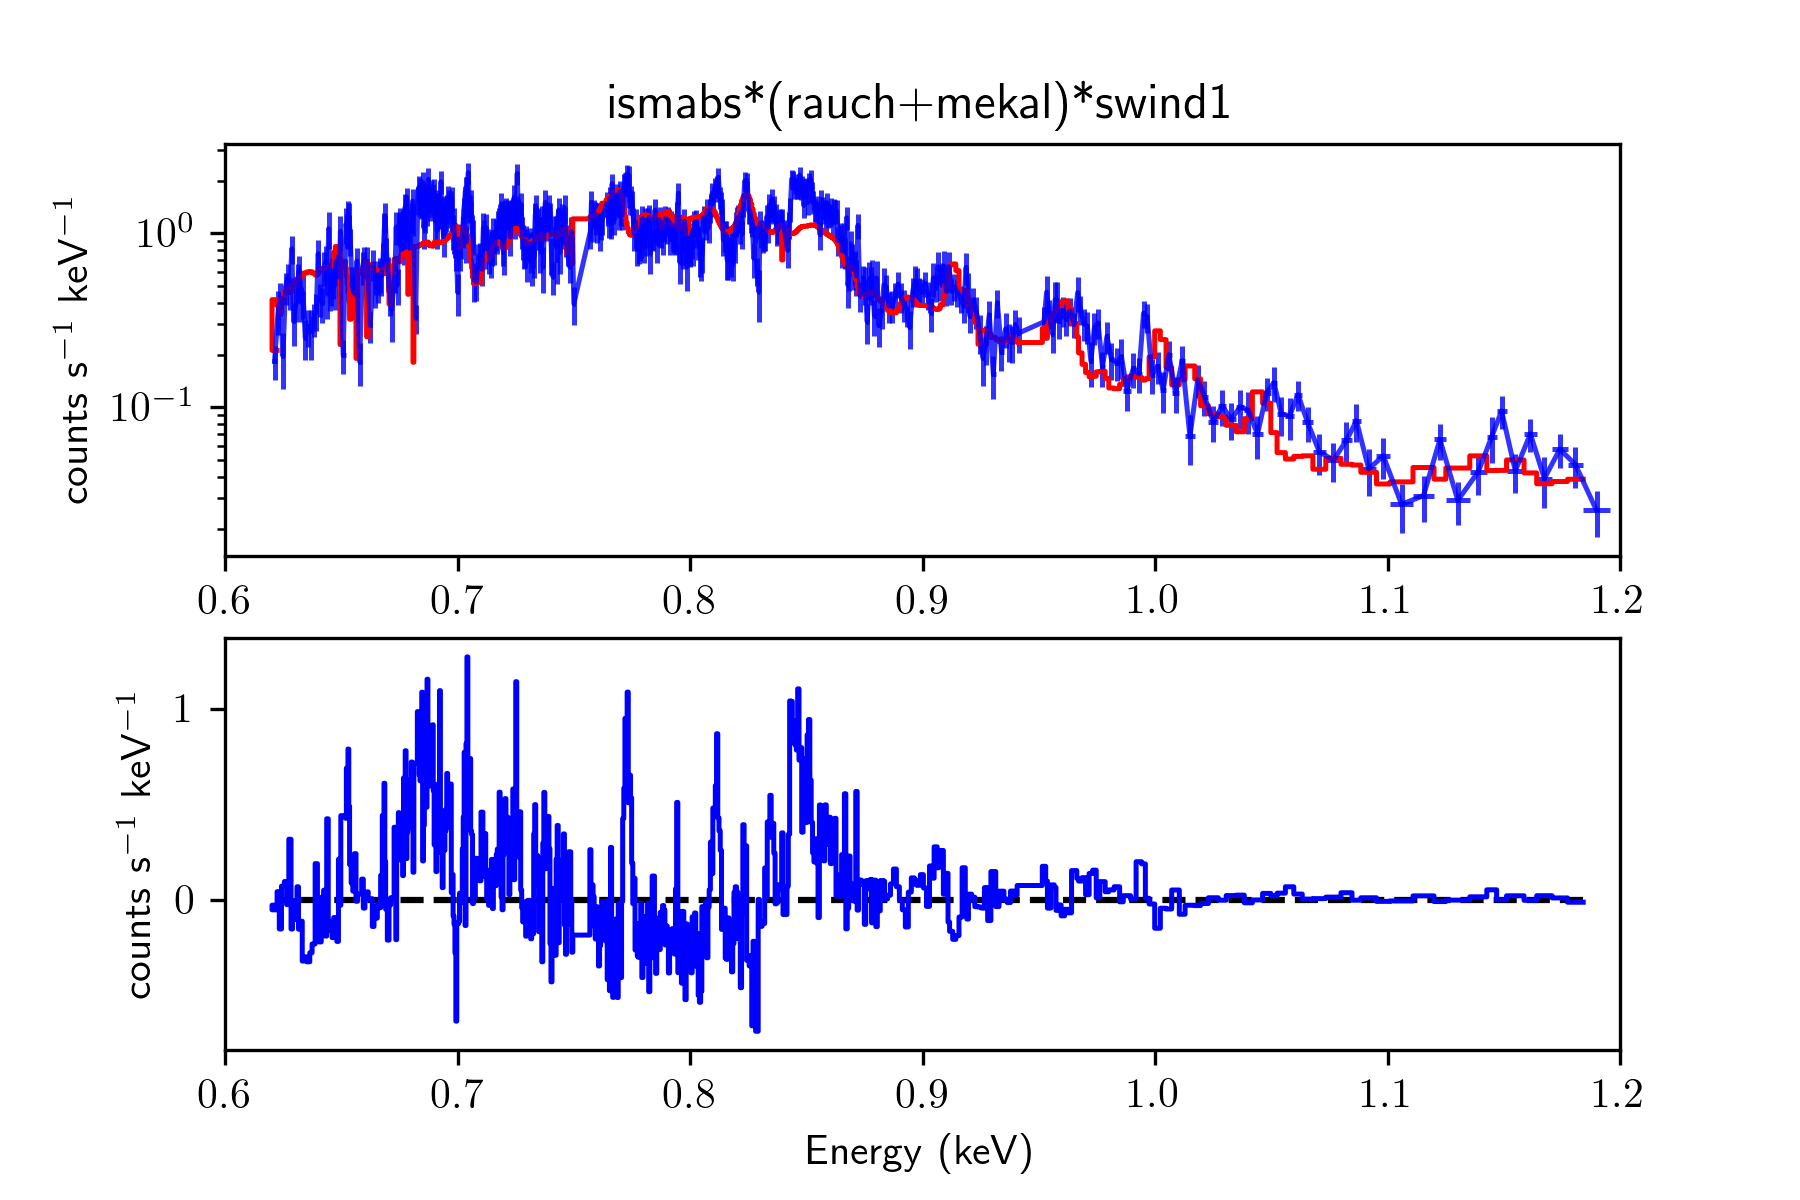
\includegraphics[width=0.45\textwidth]{mrvel-rgs2-o1-m09}} %\hfill
				\subfloat[Order 2 \label{xmm:rgs2-m09:o2}]{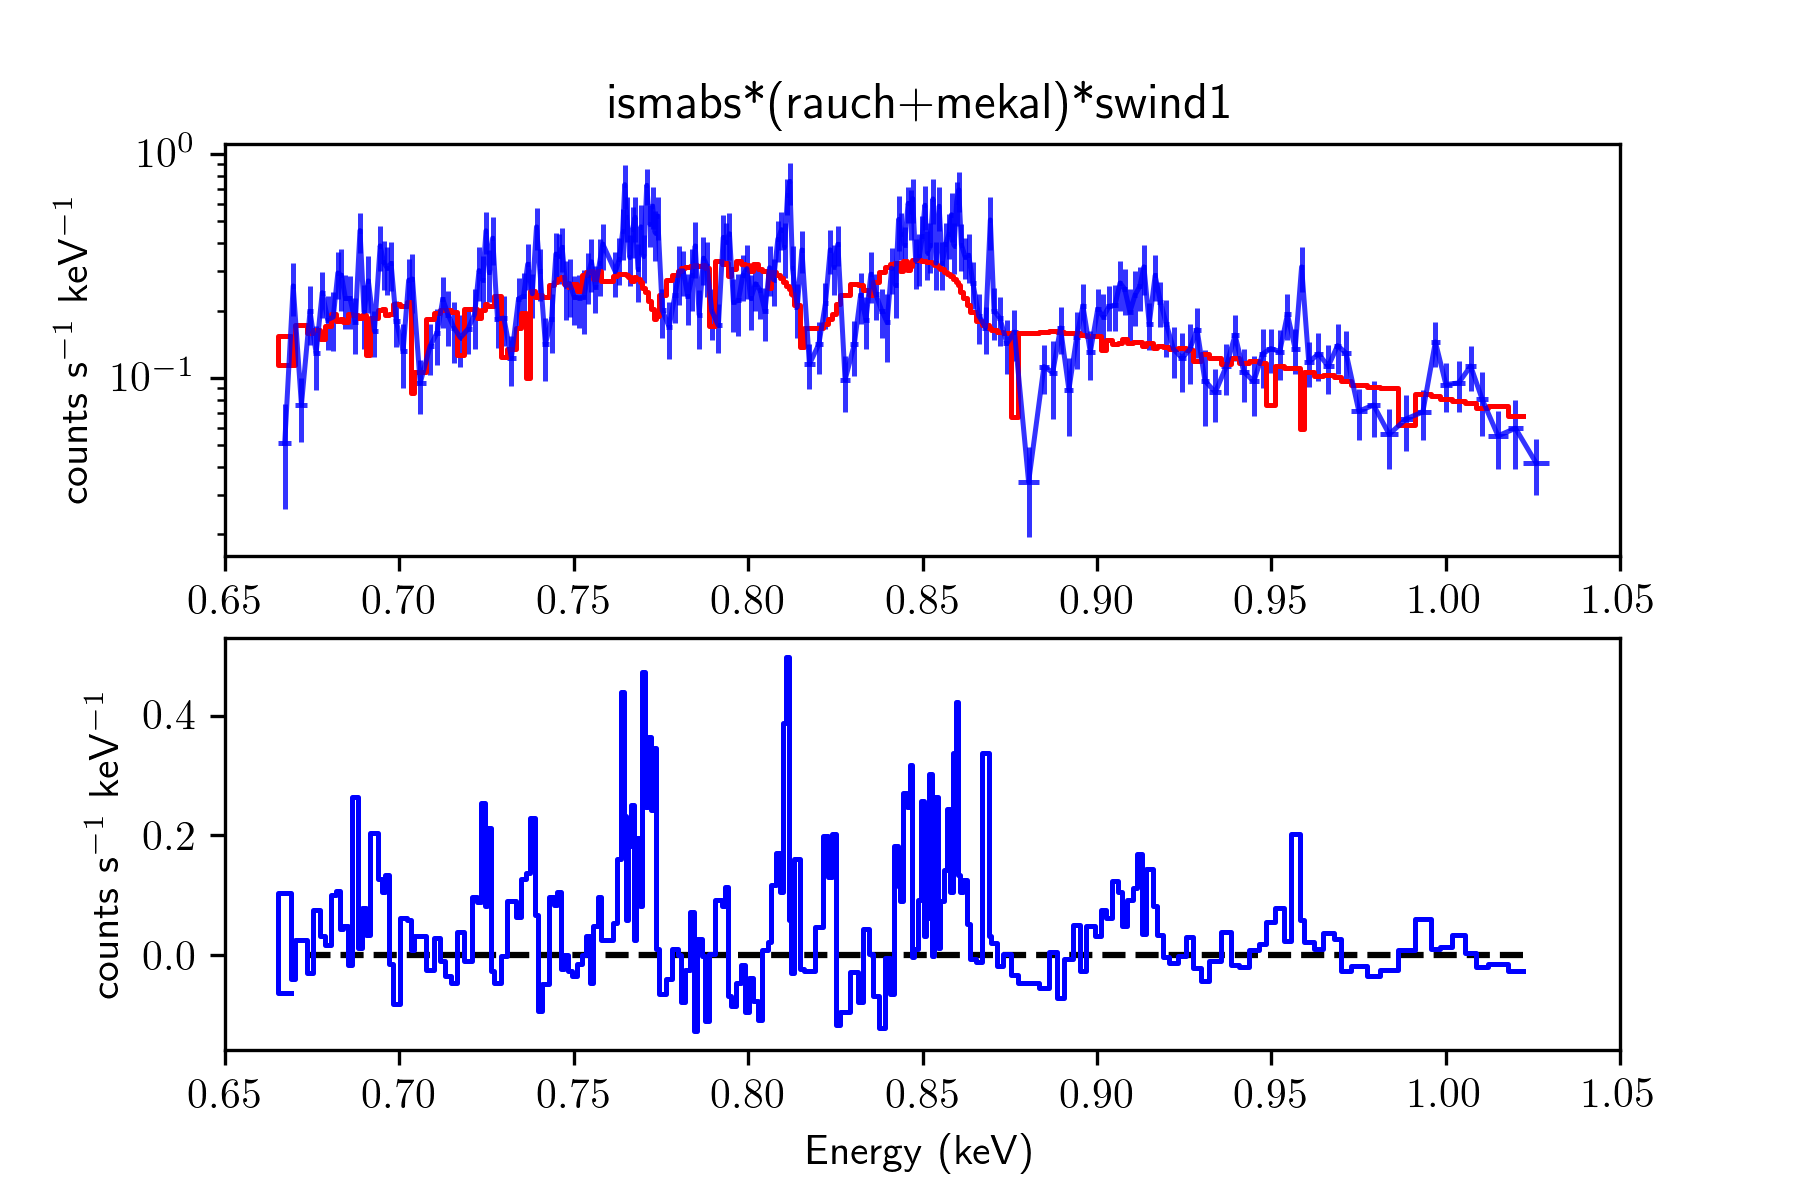
\includegraphics[width=0.45\textwidth]{mrvel-rgs2-o2-m09}} %\hfill
			\end{figure}
			\begin{figure}[h!]
				\centering
				\caption{Spectral fits for RGS2 spectra using model M10}
				\label{xmm:rgs2-m10}
				\subfloat[Order 1 \label{xmm:rgs2-m10:o1}]{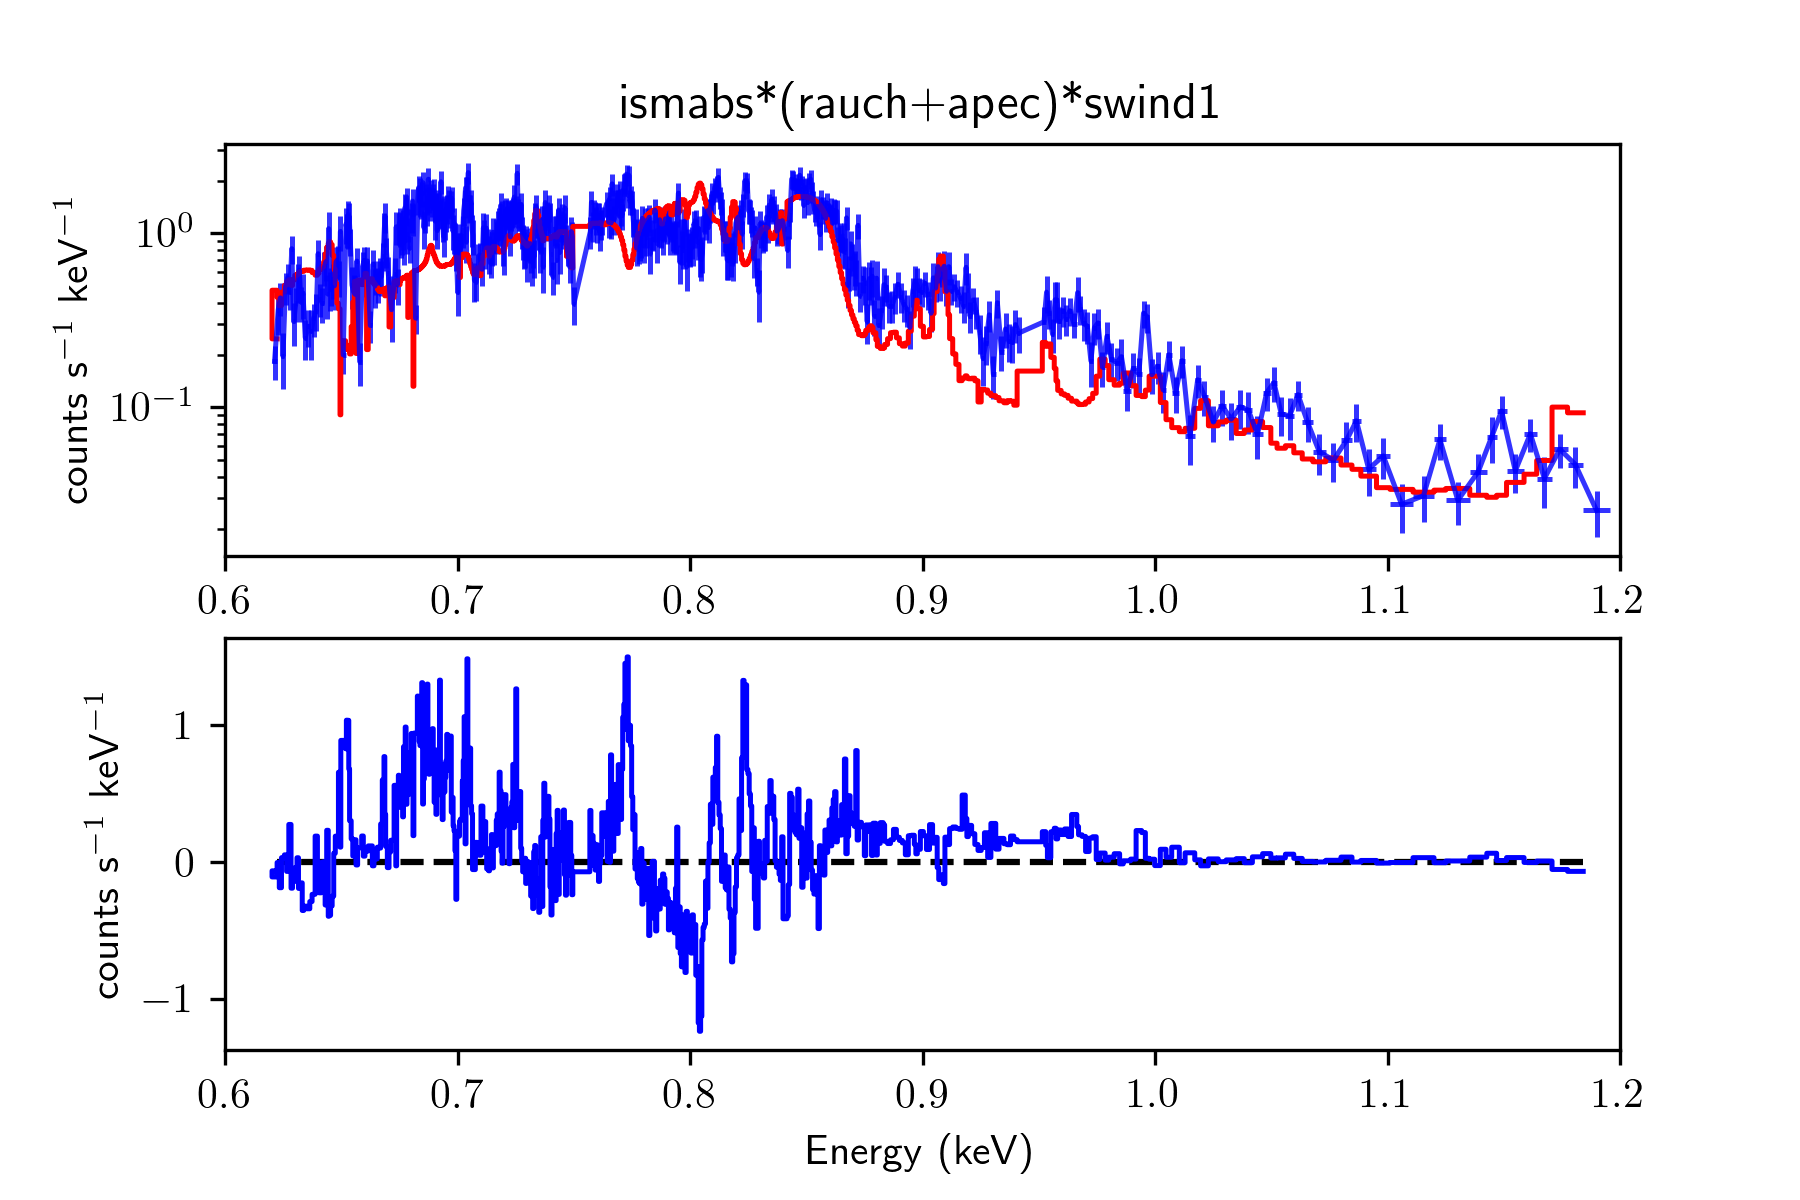
\includegraphics[width=0.45\textwidth]{mrvel-rgs2-o1-m10}} %\hfill
				\subfloat[Order 2 \label{xmm:rgs2-m10:o2}]{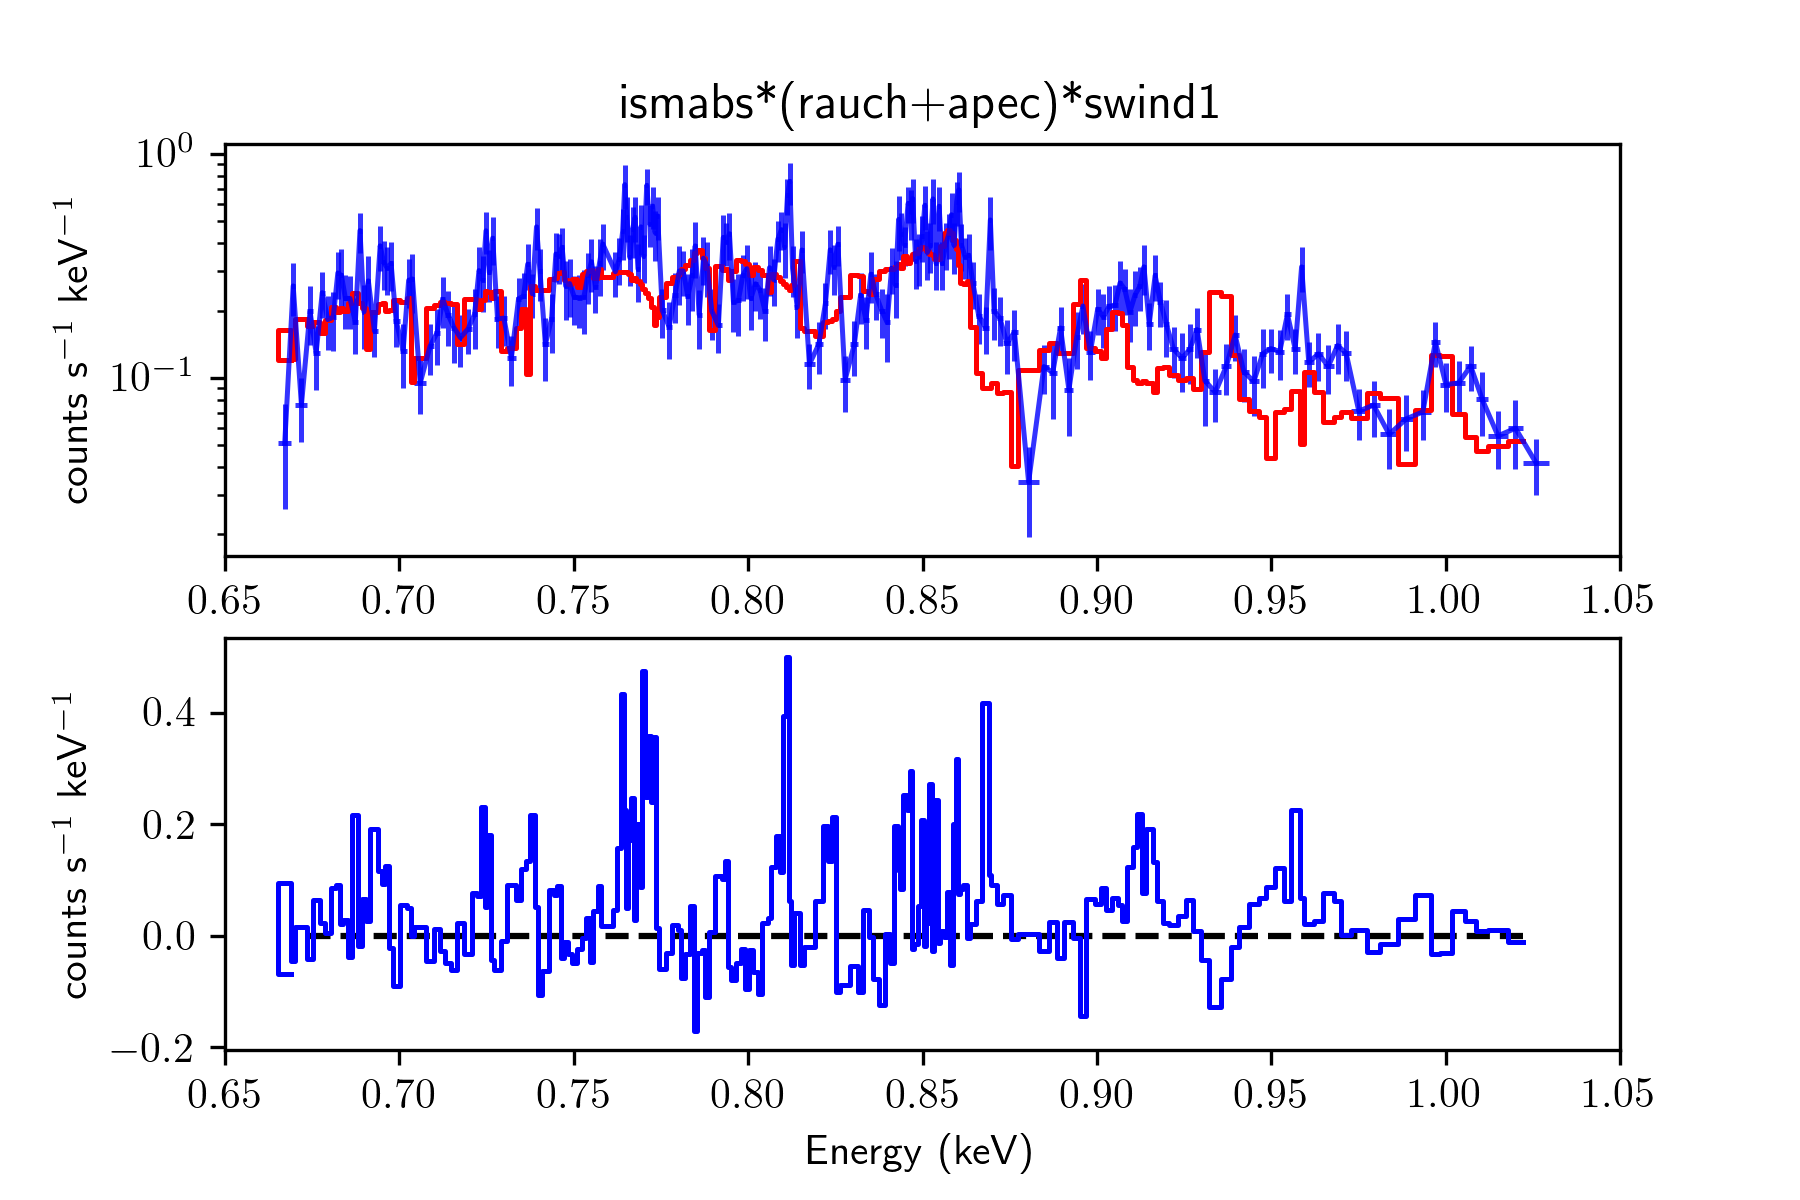
\includegraphics[width=0.45\textwidth]{mrvel-rgs2-o2-m10}} %\hfill
			\end{figure}
			\begin{figure}[h!]
				\centering
				\caption{Spectral fits for RGS2 spectra using model M11}
				\label{xmm:rgs2-m11}
				\subfloat[Order 1 \label{xmm:rgs2-m11:o1}]{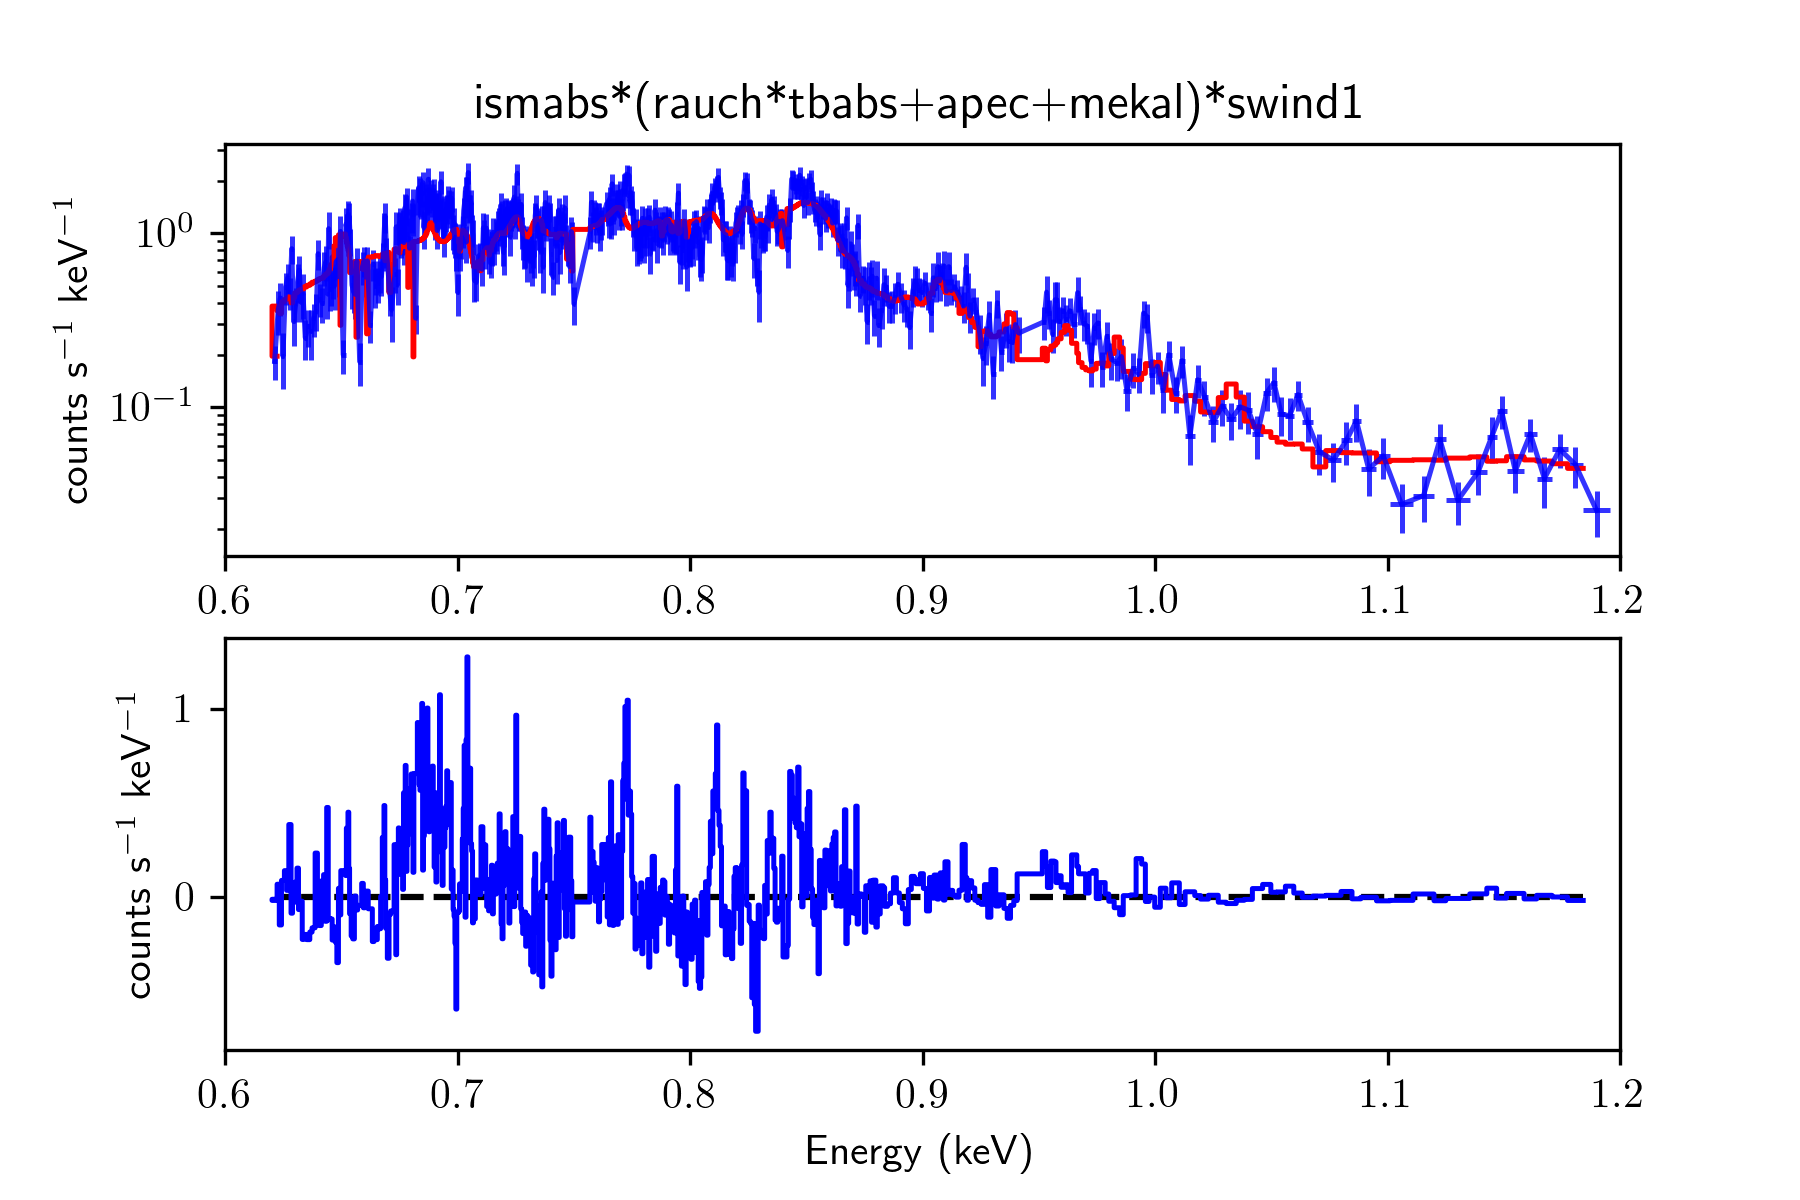
\includegraphics[width=0.45\textwidth]{mrvel-rgs2-o1-m11}} %\hfill
				\subfloat[Order 2 \label{xmm:rgs2-m11:o2}]{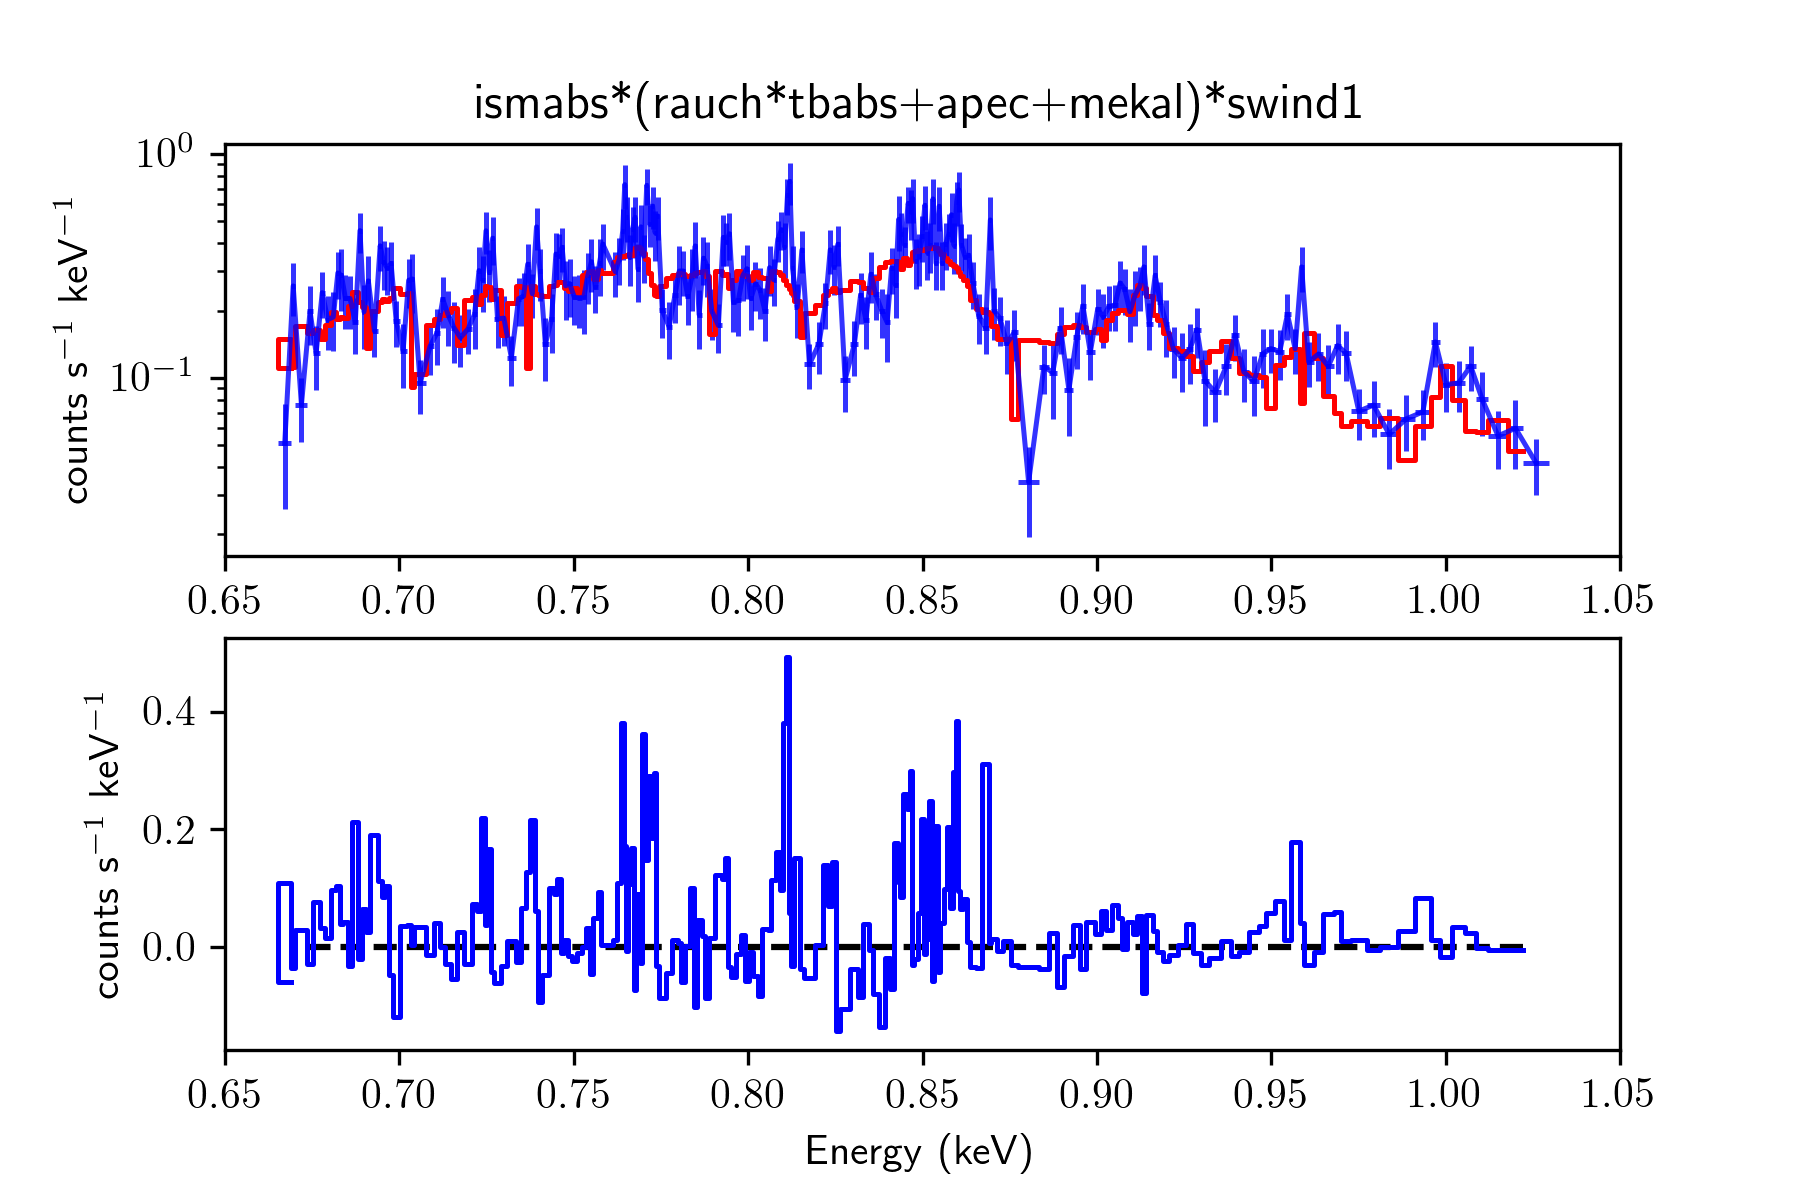
\includegraphics[width=0.45\textwidth]{mrvel-rgs2-o2-m11}} %\hfill
			\end{figure}
			\begin{figure}[h!]
				\centering
				\caption{Spectral fits for RGS2 spectra using model M12}
				\label{xmm:rgs2-m12}
				\subfloat[Order 1 \label{xmm:rgs2-m12:o1}]{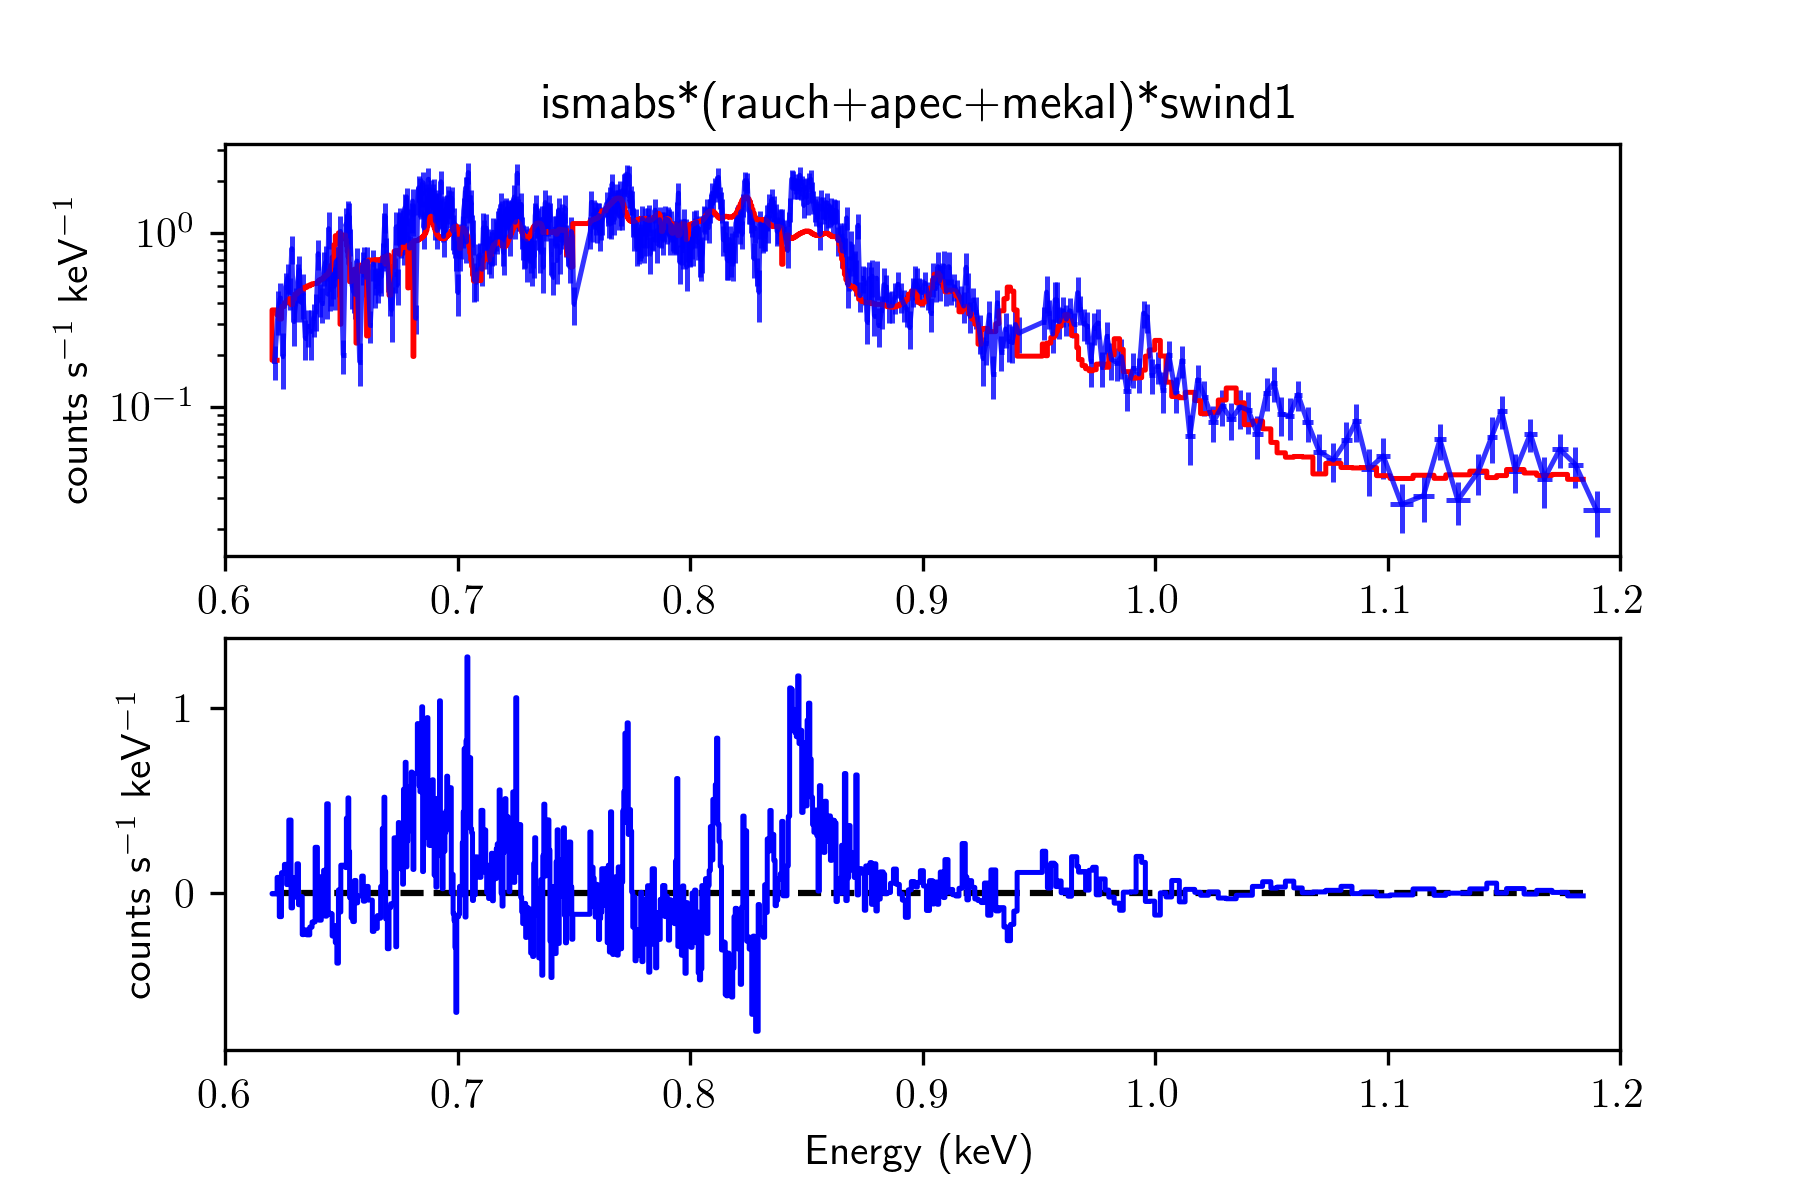
\includegraphics[width=0.45\textwidth]{mrvel-rgs2-o1-m12}} %\hfill
				\subfloat[Order 2 \label{xmm:rgs2-m12:o2}]{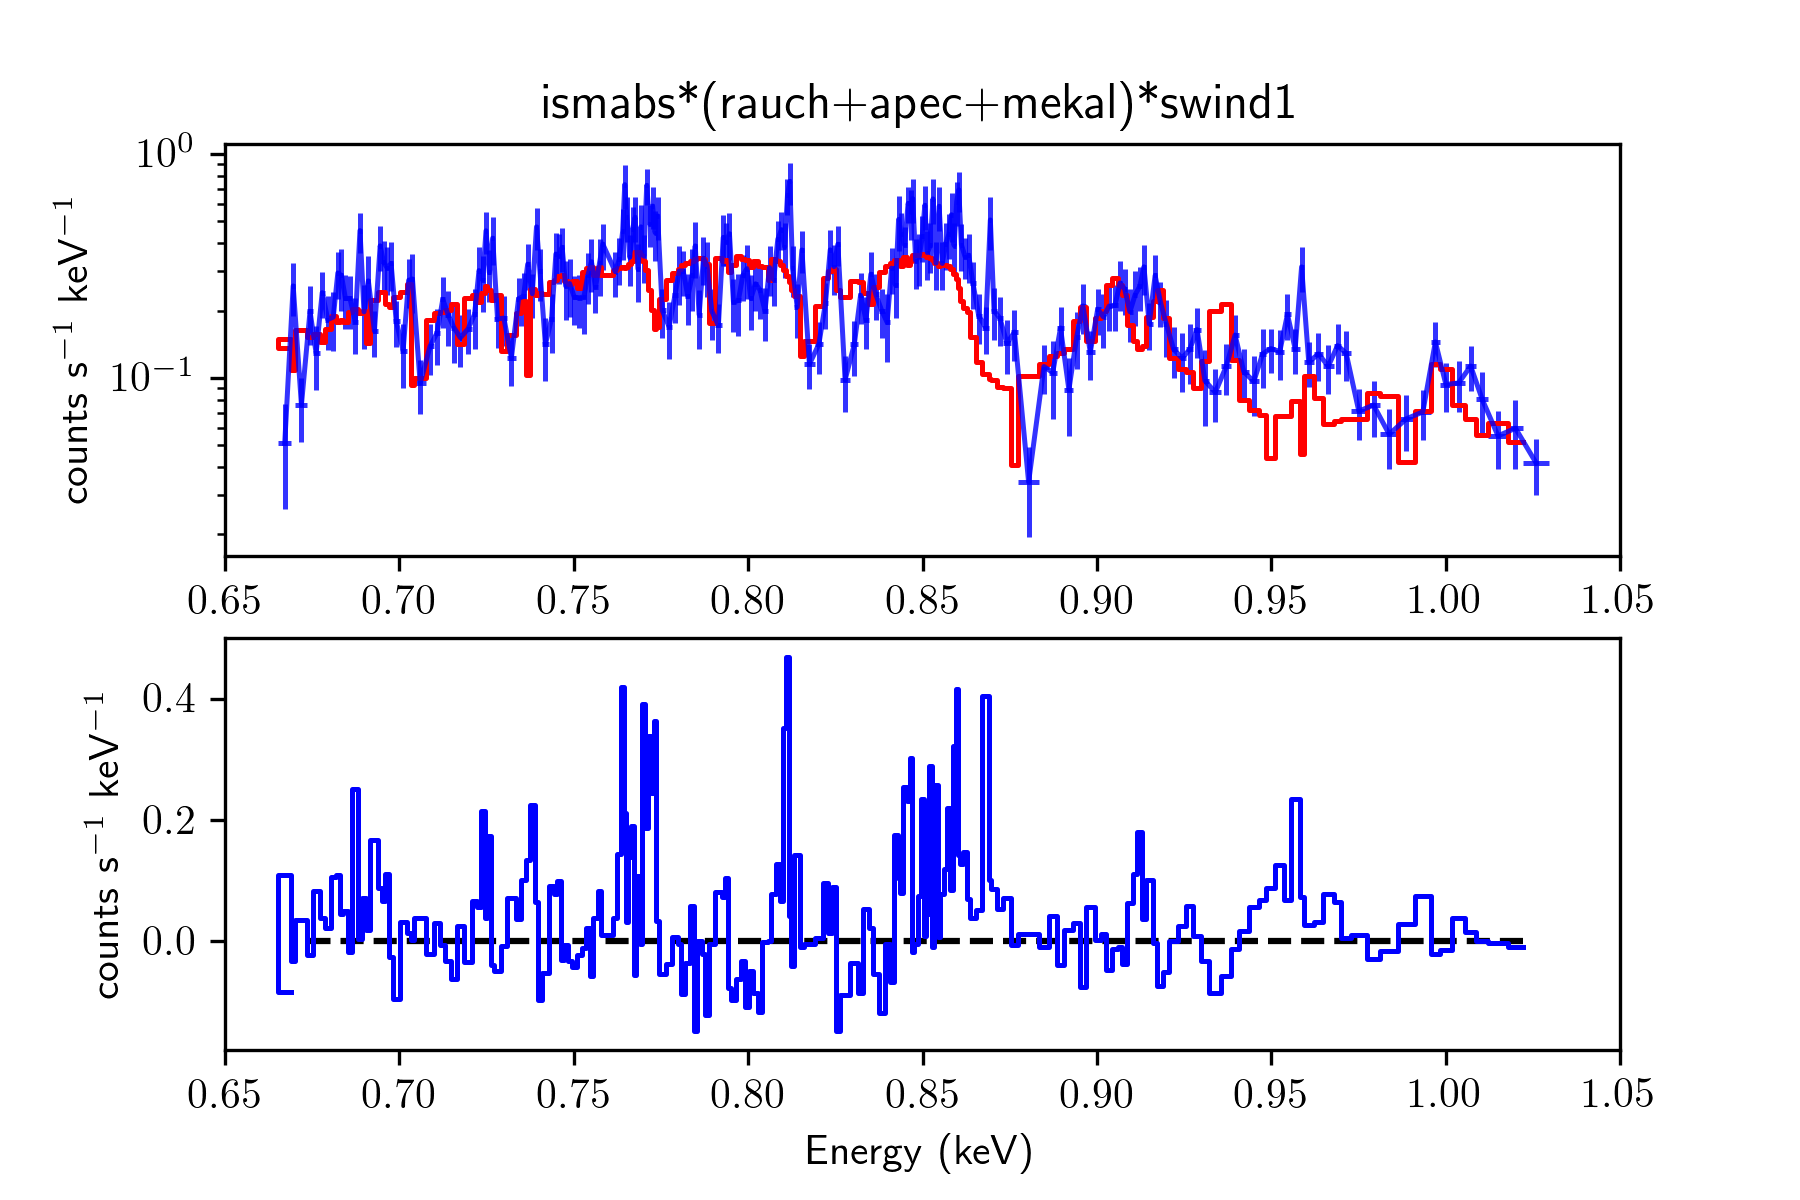
\includegraphics[width=0.45\textwidth]{mrvel-rgs2-o2-m12}} %\hfill
			\end{figure}
			
		%\subsection{With Order 1 Spectrum} \label{hi-resolution:analysis:order-1}
			%The 1$^{\mathrm{st}}$ order diffraction spectrum was fitted using the six models mentioned in \S\ref{hi-resolution:analysis} in the same order. The progression of the models increased the number of parameters, in spite of which there seems to be an improvement in the fit, as compared to those in available in literature. The best fit also seems to show significant abundances for NeI, MgI and ArI, at $2.87\times 10^{18}$, $1.10\times 10^{18}$ and $5.35\times 10^{18}$ respectively, as compared to the other metals included in the model.
			
			%\begin{figure}[h!]
			%	\centering
			%	\caption{Fitted spectrum using composite model}
			%	\subfloat[\texttt{ismabs*edge*edge*edge*(gaussian+bbody)} \label{xmm-rgs:01}]{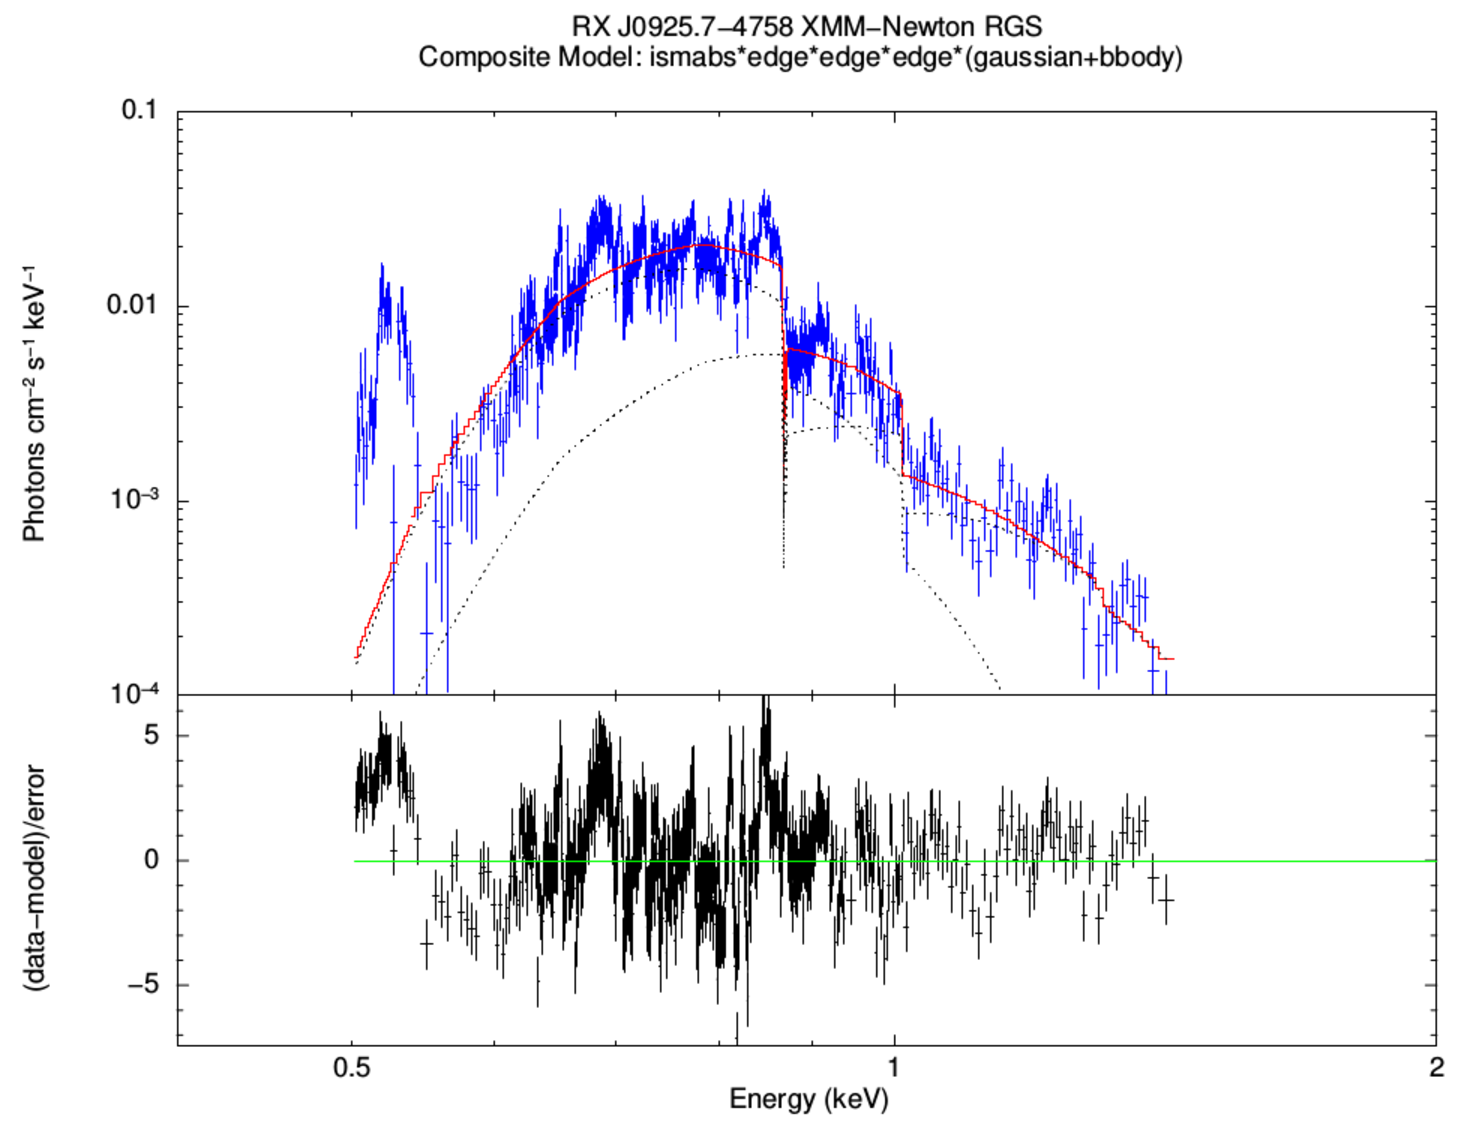
\includegraphics[scale=0.45]{mr-vel-xmm-rgs-01.pdf}}
			%\end{figure}
			
			%But there are large deviations, especially for the softer X-ray photons. This is mainly because of the fact that the current model only incorporates continuum components. To fit the large number of observed lines in the spectrum, one needs to also include model components that account for emission lines. The additive model \texttt{mekal} computes an emission spectrum from hot diffuse optical plasma (perhaps a hot corona) based on the model calculations of Mewe, Kaastra and Liedahl. The \texttt{gaussian} component is replaced with \texttt{mekal} and an attempt was made to fit the same spectrum again.
			%\begin{figure}[h!]
			%	\centering
			%	\caption{Fitted spectrum using composite model}
			%	\subfloat[\texttt{ismabs*edge*edge*edge*(mekal+bbody)} \label{xmm-rgs:02}]{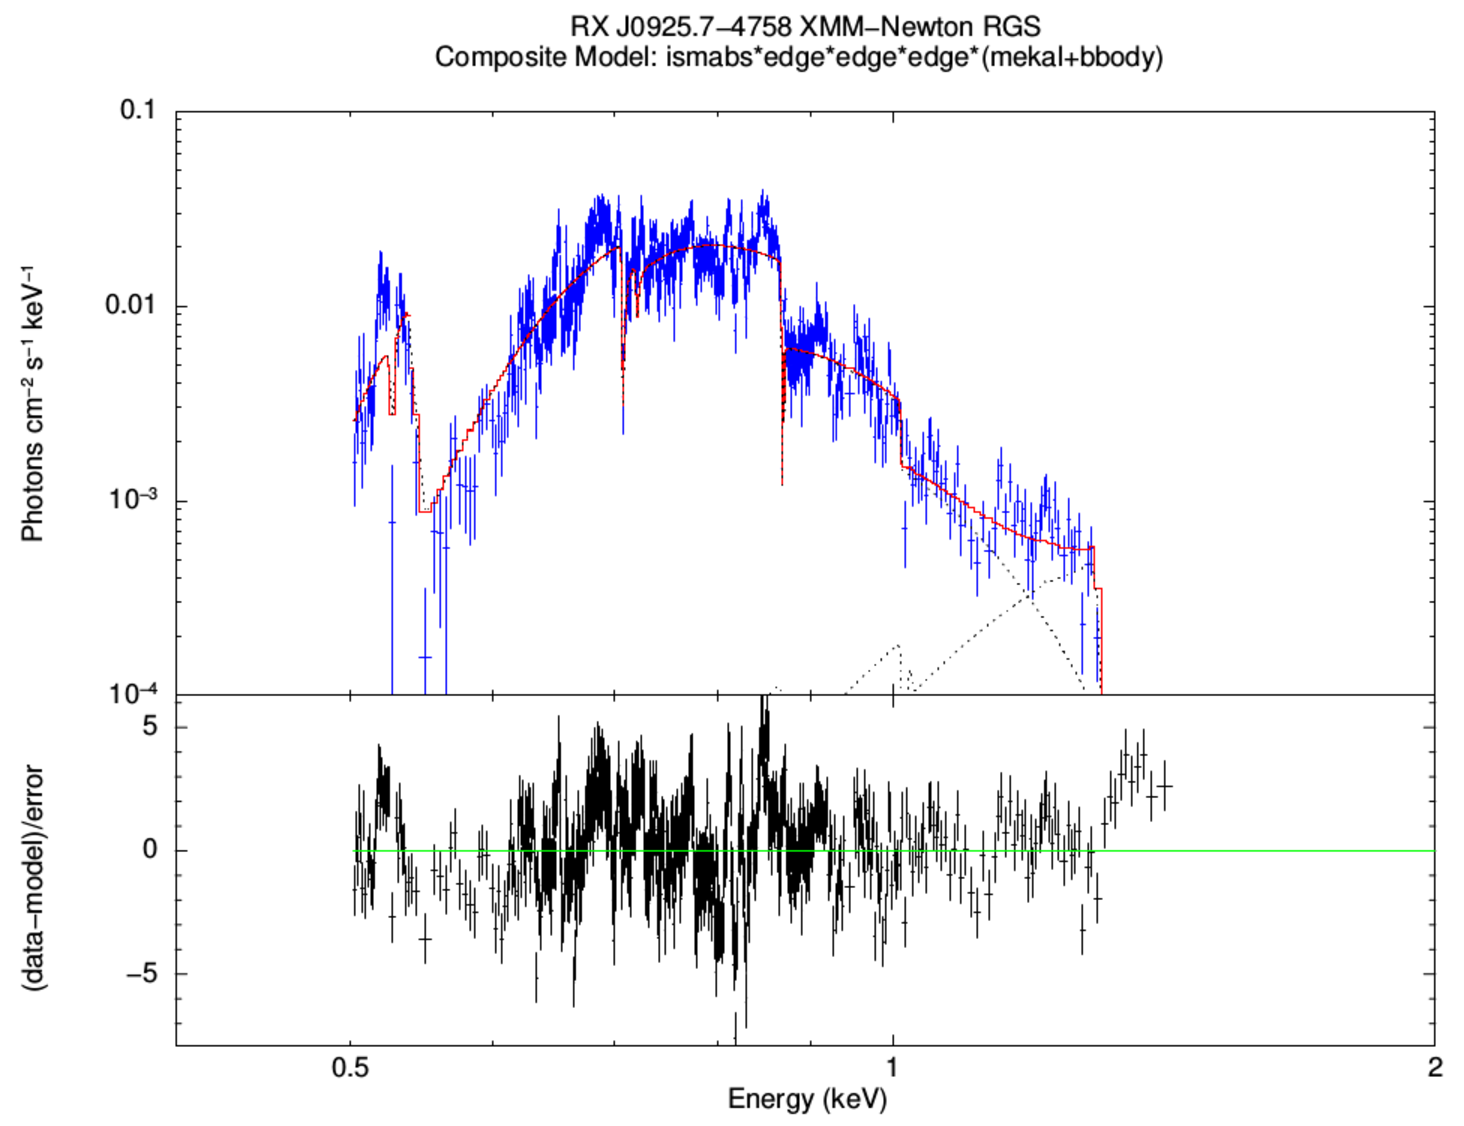
\includegraphics[scale=0.45]{mr-vel-xmm-rgs-02.pdf}}
			%\end{figure}
			
			%An improvement in the fit was observed, with a reduced $\chi^2$ value of 3.81. A visual inspection of the fitted spectrum shows that the softer photons have been accounted for with this model. This model also seems to show significant abundances for OI, NeI, MgI and SiI at $5.57\times 10^{18}$, $3.06\times 10^{18}$, $3.84\times 10^{19}$ and $7.02\times 10^{18}$ respectively.

		%\subsection{With Order 2 Spectrum} \label{hi-resolution:analysis:order-2}
			%The previous composite model was used to fit the 2$^{\mathrm{nd}}$ order diffraction spectrum, with a maximum grouping of 20 bins.
			
			%\begin{figure}[h!]
			%	\centering
			%	\caption{Fitted spectrum using composite model}
			%	\subfloat[\texttt{ismabs*edge*edge*edge*(mekal+bbody)} \label{xmm-rgs:03}]{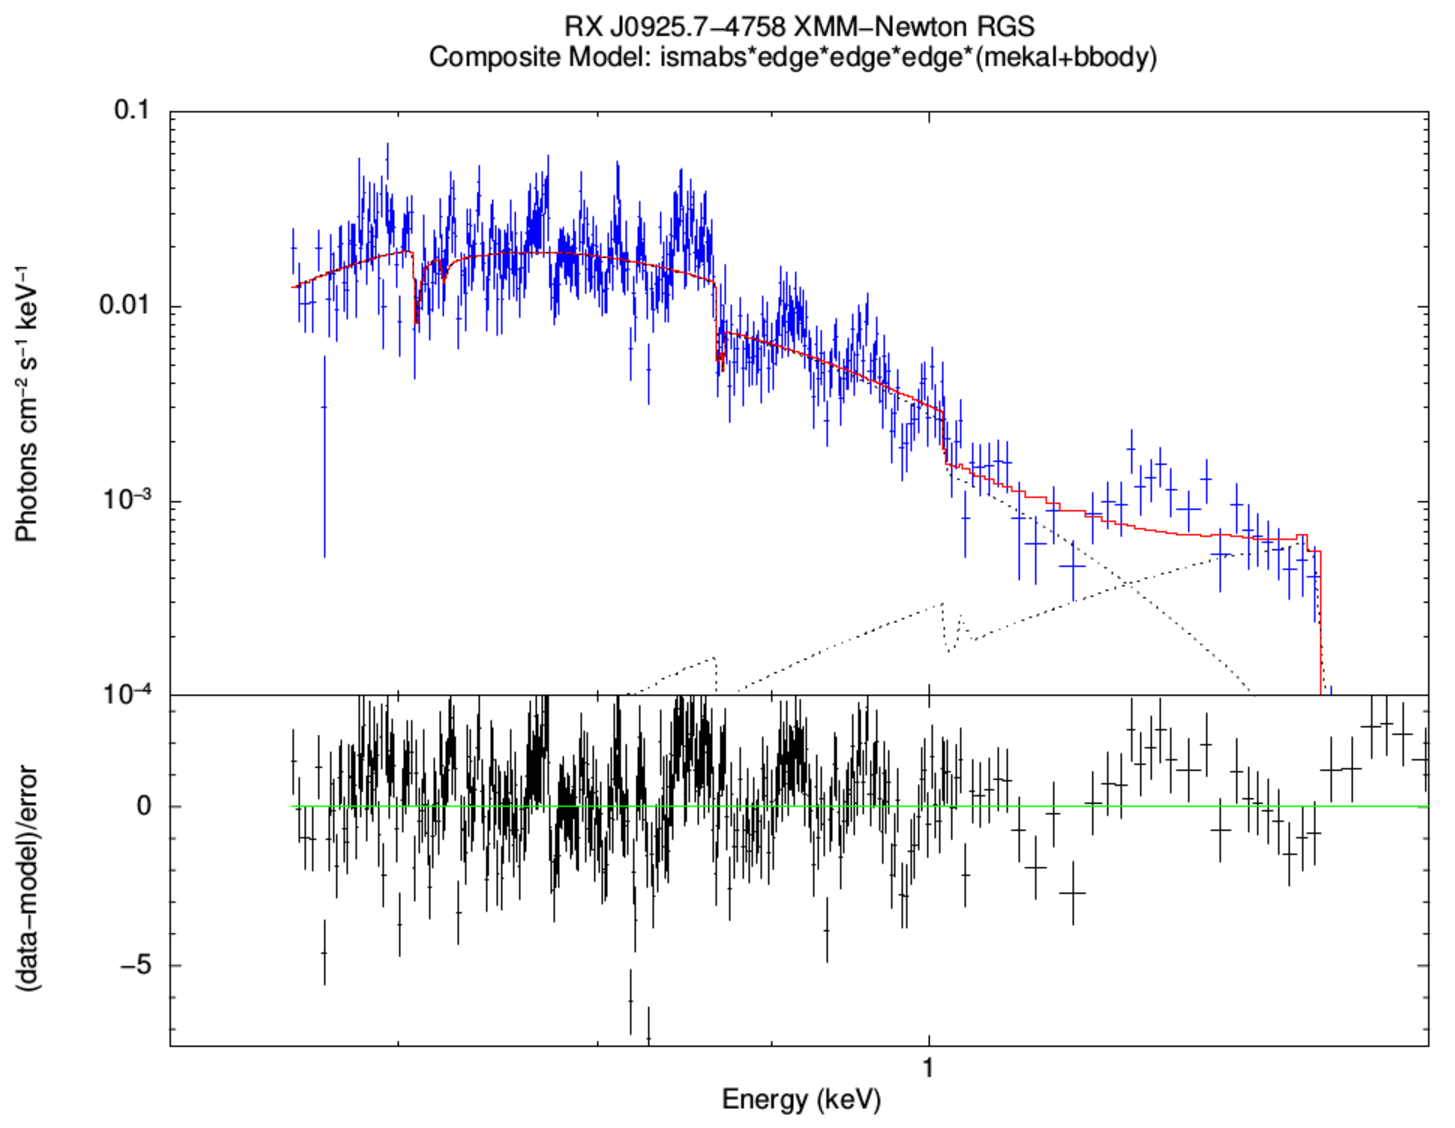
\includegraphics[scale=0.45]{mr-vel-xmm-rgs-03.pdf}}
			%\end{figure}
			
			%This spectrum showed another improvement in the fit, which is reflected in the reduced $\chi^2$ value of 2.56. This fit shows the abundances for many species. NI, OI, NeI, MgI, SiI, ArI and Fe showing abundances of $1.06\times 10^{18}$, $4.61\times 10^{18}$, $1.67\times 10^{18}$, $3.61\times 10^{19}$, $5.54\times 10^{18}$, $5.20\times 10^{16}$ and $1.31\times 10^{17}$ respectively.
			
			%However, the soft X-ray photons seen in the 1$^{\mathrm{st}}$ order spectrum seems to be missing in the  2$^{\mathrm{nd}}$ order spectrum. A fluxed spectrum comprising of data from both diffraction orders could be constructed and subsequently analysed.
